\documentclass[twoside]{book}

% Packages required by doxygen
\usepackage{calc}
\usepackage{doxygen}
\usepackage{graphicx}
\usepackage[utf8]{inputenc}
\usepackage{makeidx}
\usepackage{multicol}
\usepackage{multirow}
\usepackage{fixltx2e}
\PassOptionsToPackage{warn}{textcomp}
\usepackage{textcomp}
\usepackage[nointegrals]{wasysym}
\usepackage[table]{xcolor}

% NLS support packages
\usepackage[T2A]{fontenc}
\usepackage[russian]{babel}

% Font selection
\usepackage[T1]{fontenc}
\usepackage{mathptmx}
\usepackage[scaled=.90]{helvet}
\usepackage{courier}
\usepackage{amssymb}
\usepackage{sectsty}
\renewcommand{\familydefault}{\sfdefault}
\allsectionsfont{%
  \fontseries{bc}\selectfont%
  \color{darkgray}%
}
\renewcommand{\DoxyLabelFont}{%
  \fontseries{bc}\selectfont%
  \color{darkgray}%
}
\newcommand{\+}{\discretionary{\mbox{\scriptsize$\hookleftarrow$}}{}{}}

% Page & text layout
\usepackage{geometry}
\geometry{%
  a4paper,%
  top=2.5cm,%
  bottom=2.5cm,%
  left=2.5cm,%
  right=2.5cm%
}
\tolerance=750
\hfuzz=15pt
\hbadness=750
\setlength{\emergencystretch}{15pt}
\setlength{\parindent}{0cm}
\setlength{\parskip}{0.2cm}
\makeatletter
\renewcommand{\paragraph}{%
  \@startsection{paragraph}{4}{0ex}{-1.0ex}{1.0ex}{%
    \normalfont\normalsize\bfseries\SS@parafont%
  }%
}
\renewcommand{\subparagraph}{%
  \@startsection{subparagraph}{5}{0ex}{-1.0ex}{1.0ex}{%
    \normalfont\normalsize\bfseries\SS@subparafont%
  }%
}
\makeatother

% Headers & footers
\usepackage{fancyhdr}
\pagestyle{fancyplain}
\fancyhead[LE]{\fancyplain{}{\bfseries\thepage}}
\fancyhead[CE]{\fancyplain{}{}}
\fancyhead[RE]{\fancyplain{}{\bfseries\leftmark}}
\fancyhead[LO]{\fancyplain{}{\bfseries\rightmark}}
\fancyhead[CO]{\fancyplain{}{}}
\fancyhead[RO]{\fancyplain{}{\bfseries\thepage}}
\fancyfoot[LE]{\fancyplain{}{}}
\fancyfoot[CE]{\fancyplain{}{}}
\fancyfoot[RE]{\fancyplain{}{\bfseries\scriptsize Документация по Automoto. Последние изменения\+: Вт 3 Июн 2014 07\+:25\+:25. Создано системой Doxygen }}
\fancyfoot[LO]{\fancyplain{}{\bfseries\scriptsize Документация по Automoto. Последние изменения\+: Вт 3 Июн 2014 07\+:25\+:25. Создано системой Doxygen }}
\fancyfoot[CO]{\fancyplain{}{}}
\fancyfoot[RO]{\fancyplain{}{}}
\renewcommand{\footrulewidth}{0.4pt}
\renewcommand{\chaptermark}[1]{%
  \markboth{#1}{}%
}
\renewcommand{\sectionmark}[1]{%
  \markright{\thesection\ #1}%
}

% Indices & bibliography
\usepackage{natbib}
\usepackage[titles]{tocloft}
\setcounter{tocdepth}{3}
\setcounter{secnumdepth}{5}
\makeindex

% Hyperlinks (required, but should be loaded last)
\usepackage{ifpdf}
\ifpdf
  \usepackage[pdftex,pagebackref=true]{hyperref}
\else
  \usepackage[ps2pdf,pagebackref=true]{hyperref}
\fi
\hypersetup{%
  colorlinks=true,%
  linkcolor=blue,%
  citecolor=blue,%
  unicode%
}

% Custom commands
\newcommand{\clearemptydoublepage}{%
  \newpage{\pagestyle{empty}\cleardoublepage}%
}


%===== C O N T E N T S =====

\begin{document}

% Titlepage & ToC
\hypersetup{pageanchor=false,
             bookmarks=true,
             bookmarksnumbered=true,
             pdfencoding=unicode
            }
\pagenumbering{roman}
\begin{titlepage}
\vspace*{7cm}
\begin{center}%
{\Large Automoto \\[1ex]\large 1 }\\
\vspace*{1cm}
{\large Создано системой Doxygen 1.8.7}\\
\vspace*{0.5cm}
{\small Вт 3 Июн 2014 07:25:25}\\
\end{center}
\end{titlepage}
\clearemptydoublepage
\tableofcontents
\clearemptydoublepage
\pagenumbering{arabic}
\hypersetup{pageanchor=true}

%--- Begin generated contents ---
\chapter{Алфавитный указатель пространств имен}
\section{Пространства имен}
Полный список документированных пространств имен.\begin{DoxyCompactList}
\item\contentsline{section}{\hyperlink{namespace_r_t}{R\+T} }{\pageref{namespace_r_t}}{}
\item\contentsline{section}{\hyperlink{namespace_r_t_1_1_parsing_libs}{R\+T.\+Parsing\+Libs} }{\pageref{namespace_r_t_1_1_parsing_libs}}{}
\item\contentsline{section}{\hyperlink{namespace_r_t_1_1_parsing_libs_1_1_models}{R\+T.\+Parsing\+Libs.\+Models} }{\pageref{namespace_r_t_1_1_parsing_libs_1_1_models}}{}
\end{DoxyCompactList}

\chapter{Иерархический список классов}
\section{Иерархия классов}
Иерархия классов.\begin{DoxyCompactList}
\item \contentsline{section}{R\+T.\+Parsing\+Libs.\+Models.\+Additional\+Info}{\pageref{class_r_t_1_1_parsing_libs_1_1_models_1_1_additional_info}}{}
\item \contentsline{section}{R\+T.\+Parsing\+Libs.\+Models.\+Automoto\+Additional\+Info}{\pageref{class_r_t_1_1_parsing_libs_1_1_models_1_1_automoto_additional_info}}{}
\item \contentsline{section}{R\+T.\+Parsing\+Libs.\+Models.\+Namespace\+Doc}{\pageref{class_r_t_1_1_parsing_libs_1_1_models_1_1_namespace_doc}}{}
\item Object\begin{DoxyCompactList}
\item \contentsline{section}{R\+T.\+Parsing\+Libs.\+Models.\+Bind}{\pageref{class_r_t_1_1_parsing_libs_1_1_models_1_1_bind}}{}
\end{DoxyCompactList}
\item \contentsline{section}{R\+T.\+Parsing\+Libs.\+Models.\+Realty\+Additional\+Info}{\pageref{class_r_t_1_1_parsing_libs_1_1_models_1_1_realty_additional_info}}{}
\item \contentsline{section}{R\+T.\+Parsing\+Libs.\+Models.\+Web\+Publication}{\pageref{class_r_t_1_1_parsing_libs_1_1_models_1_1_web_publication}}{}
\item \contentsline{section}{R\+T.\+Parsing\+Libs.\+Models.\+Web\+Publication\+Contact}{\pageref{class_r_t_1_1_parsing_libs_1_1_models_1_1_web_publication_contact}}{}
\end{DoxyCompactList}

\chapter{Алфавитный указатель классов}
\section{Классы}
Классы с их кратким описанием.\begin{DoxyCompactList}
\item\contentsline{section}{\hyperlink{class_r_t_1_1_parsing_libs_1_1_models_1_1_additional_info}{R\+T.\+Parsing\+Libs.\+Models.\+Additional\+Info} \\*Дополнительная информация специфичная для каждой рубрики }{\pageref{class_r_t_1_1_parsing_libs_1_1_models_1_1_additional_info}}{}
\item\contentsline{section}{\hyperlink{class_r_t_1_1_parsing_libs_1_1_models_1_1_automoto_additional_info}{R\+T.\+Parsing\+Libs.\+Models.\+Automoto\+Additional\+Info} \\*Дополнительная информация для рубрики \char`\"{}Транспортные средства\char`\"{} }{\pageref{class_r_t_1_1_parsing_libs_1_1_models_1_1_automoto_additional_info}}{}
\item\contentsline{section}{\hyperlink{class_r_t_1_1_parsing_libs_1_1_models_1_1_bind}{R\+T.\+Parsing\+Libs.\+Models.\+Bind} \\*Бинд (тройка ИД рубрика-\/регион-\/действие) }{\pageref{class_r_t_1_1_parsing_libs_1_1_models_1_1_bind}}{}
\item\contentsline{section}{\hyperlink{class_r_t_1_1_parsing_libs_1_1_models_1_1_namespace_doc}{R\+T.\+Parsing\+Libs.\+Models.\+Namespace\+Doc} \\*\hyperlink{namespace_r_t_1_1_parsing_libs_1_1_models}{R\+T.\+Parsing\+Libs.\+Models} пространство содержит базовые модели для парсеров }{\pageref{class_r_t_1_1_parsing_libs_1_1_models_1_1_namespace_doc}}{}
\item\contentsline{section}{\hyperlink{class_r_t_1_1_parsing_libs_1_1_models_1_1_realty_additional_info}{R\+T.\+Parsing\+Libs.\+Models.\+Realty\+Additional\+Info} \\*Дополнительная информация для рубрики \char`\"{}Недвижимость\char`\"{} }{\pageref{class_r_t_1_1_parsing_libs_1_1_models_1_1_realty_additional_info}}{}
\item\contentsline{section}{\hyperlink{class_r_t_1_1_parsing_libs_1_1_models_1_1_web_publication}{R\+T.\+Parsing\+Libs.\+Models.\+Web\+Publication} \\*Объявление }{\pageref{class_r_t_1_1_parsing_libs_1_1_models_1_1_web_publication}}{}
\item\contentsline{section}{\hyperlink{class_r_t_1_1_parsing_libs_1_1_models_1_1_web_publication_contact}{R\+T.\+Parsing\+Libs.\+Models.\+Web\+Publication\+Contact} \\*Контактная информация объявления }{\pageref{class_r_t_1_1_parsing_libs_1_1_models_1_1_web_publication_contact}}{}
\end{DoxyCompactList}

\chapter{Пространства имен}
\hypertarget{namespace_r_t}{\section{Пакет R\+T}
\label{namespace_r_t}\index{R\+T@{R\+T}}
}
\subsection*{Пространства имен}
\begin{DoxyCompactItemize}
\item 
package \hyperlink{namespace_r_t_1_1_parsing_libs}{Parsing\+Libs}
\end{DoxyCompactItemize}

\hypertarget{namespace_r_t_1_1_parsing_libs}{\section{Пакет R\+T.\+Parsing\+Libs}
\label{namespace_r_t_1_1_parsing_libs}\index{R\+T.\+Parsing\+Libs@{R\+T.\+Parsing\+Libs}}
}
\subsection*{Пространства имен}
\begin{DoxyCompactItemize}
\item 
package \hyperlink{namespace_r_t_1_1_parsing_libs_1_1_models}{Models}
\end{DoxyCompactItemize}

\hypertarget{namespace_r_t_1_1_parsing_libs_1_1_models}{\section{Пакет R\+T.\+Parsing\+Libs.\+Models}
\label{namespace_r_t_1_1_parsing_libs_1_1_models}\index{R\+T.\+Parsing\+Libs.\+Models@{R\+T.\+Parsing\+Libs.\+Models}}
}
\subsection*{Классы}
\begin{DoxyCompactItemize}
\item 
class \hyperlink{class_r_t_1_1_parsing_libs_1_1_models_1_1_additional_info}{Additional\+Info}
\begin{DoxyCompactList}\small\item\em Дополнительная информация специфичная для каждой рубрики \end{DoxyCompactList}\item 
class \hyperlink{class_r_t_1_1_parsing_libs_1_1_models_1_1_automoto_additional_info}{Automoto\+Additional\+Info}
\begin{DoxyCompactList}\small\item\em Дополнительная информация для рубрики \char`\"{}Транспортные средства\char`\"{} \end{DoxyCompactList}\item 
class \hyperlink{class_r_t_1_1_parsing_libs_1_1_models_1_1_bind}{Bind}
\begin{DoxyCompactList}\small\item\em Бинд (тройка ИД рубрика-\/регион-\/действие) \end{DoxyCompactList}\item 
class \hyperlink{class_r_t_1_1_parsing_libs_1_1_models_1_1_namespace_doc}{Namespace\+Doc}
\begin{DoxyCompactList}\small\item\em \hyperlink{namespace_r_t_1_1_parsing_libs_1_1_models}{R\+T.\+Parsing\+Libs.\+Models} пространство содержит базовые модели для парсеров \end{DoxyCompactList}\item 
class \hyperlink{class_r_t_1_1_parsing_libs_1_1_models_1_1_realty_additional_info}{Realty\+Additional\+Info}
\begin{DoxyCompactList}\small\item\em Дополнительная информация для рубрики \char`\"{}Недвижимость\char`\"{} \end{DoxyCompactList}\item 
class \hyperlink{class_r_t_1_1_parsing_libs_1_1_models_1_1_web_publication}{Web\+Publication}
\begin{DoxyCompactList}\small\item\em Объявление \end{DoxyCompactList}\item 
class \hyperlink{class_r_t_1_1_parsing_libs_1_1_models_1_1_web_publication_contact}{Web\+Publication\+Contact}
\begin{DoxyCompactList}\small\item\em Контактная информация объявления \end{DoxyCompactList}\end{DoxyCompactItemize}
\subsection*{Перечисления}
\begin{DoxyCompactItemize}
\item 
enum \hyperlink{namespace_r_t_1_1_parsing_libs_1_1_models_a7941eaea5a5a6680ee94d4b34a5cf9ef}{Parse\+Response\+Code} \{ \\*
\hyperlink{namespace_r_t_1_1_parsing_libs_1_1_models_a7941eaea5a5a6680ee94d4b34a5cf9efa505a83f220c02df2f85c3810cd9ceb38}{Parse\+Response\+Code.\+Success} = 0, 
\hyperlink{namespace_r_t_1_1_parsing_libs_1_1_models_a7941eaea5a5a6680ee94d4b34a5cf9efa7d42ab672fe4c968e726d7ea65ce8ab4}{Parse\+Response\+Code.\+Ban\+Resource} = 1, 
\hyperlink{namespace_r_t_1_1_parsing_libs_1_1_models_a7941eaea5a5a6680ee94d4b34a5cf9efabece6ab883cc5b9f5da0ce1e510aa7a7}{Parse\+Response\+Code.\+Content\+Chage} = 2, 
\hyperlink{namespace_r_t_1_1_parsing_libs_1_1_models_a7941eaea5a5a6680ee94d4b34a5cf9efa266eac857b2b6c0699e36bd61c6ac00d}{Parse\+Response\+Code.\+Content\+Empty} = 3, 
\\*
\hyperlink{namespace_r_t_1_1_parsing_libs_1_1_models_a7941eaea5a5a6680ee94d4b34a5cf9efaa6ce52e397059af52041cb679334651e}{Parse\+Response\+Code.\+Not\+Available\+Resource} = 4, 
\hyperlink{namespace_r_t_1_1_parsing_libs_1_1_models_a7941eaea5a5a6680ee94d4b34a5cf9efa5fa868a7917df75189439af1d7084b69}{Parse\+Response\+Code.\+Not\+Found\+Id} = 5
 \}
\begin{DoxyCompactList}\small\item\em Код результата работы \end{DoxyCompactList}\end{DoxyCompactItemize}


\subsection{Перечисления}
\hypertarget{namespace_r_t_1_1_parsing_libs_1_1_models_a7941eaea5a5a6680ee94d4b34a5cf9ef}{\index{R\+T\+::\+Parsing\+Libs\+::\+Models@{R\+T\+::\+Parsing\+Libs\+::\+Models}!Parse\+Response\+Code@{Parse\+Response\+Code}}
\index{Parse\+Response\+Code@{Parse\+Response\+Code}!R\+T\+::\+Parsing\+Libs\+::\+Models@{R\+T\+::\+Parsing\+Libs\+::\+Models}}
\subsubsection[{Parse\+Response\+Code}]{\setlength{\rightskip}{0pt plus 5cm}enum {\bf R\+T.\+Parsing\+Libs.\+Models.\+Parse\+Response\+Code}}}\label{namespace_r_t_1_1_parsing_libs_1_1_models_a7941eaea5a5a6680ee94d4b34a5cf9ef}


Код результата работы 

\begin{Desc}
\item[Элементы перечислений]\par
\begin{description}
\index{Success@{Success}!R\+T\+::\+Parsing\+Libs\+::\+Models@{R\+T\+::\+Parsing\+Libs\+::\+Models}}\index{R\+T\+::\+Parsing\+Libs\+::\+Models@{R\+T\+::\+Parsing\+Libs\+::\+Models}!Success@{Success}}\item[{\em 
\hypertarget{namespace_r_t_1_1_parsing_libs_1_1_models_a7941eaea5a5a6680ee94d4b34a5cf9efa505a83f220c02df2f85c3810cd9ceb38}{Success}\label{namespace_r_t_1_1_parsing_libs_1_1_models_a7941eaea5a5a6680ee94d4b34a5cf9efa505a83f220c02df2f85c3810cd9ceb38}
}]Успешная обработка \index{Ban\+Resource@{Ban\+Resource}!R\+T\+::\+Parsing\+Libs\+::\+Models@{R\+T\+::\+Parsing\+Libs\+::\+Models}}\index{R\+T\+::\+Parsing\+Libs\+::\+Models@{R\+T\+::\+Parsing\+Libs\+::\+Models}!Ban\+Resource@{Ban\+Resource}}\item[{\em 
\hypertarget{namespace_r_t_1_1_parsing_libs_1_1_models_a7941eaea5a5a6680ee94d4b34a5cf9efa7d42ab672fe4c968e726d7ea65ce8ab4}{Ban\+Resource}\label{namespace_r_t_1_1_parsing_libs_1_1_models_a7941eaea5a5a6680ee94d4b34a5cf9efa7d42ab672fe4c968e726d7ea65ce8ab4}
}]Бан сайта \index{Content\+Chage@{Content\+Chage}!R\+T\+::\+Parsing\+Libs\+::\+Models@{R\+T\+::\+Parsing\+Libs\+::\+Models}}\index{R\+T\+::\+Parsing\+Libs\+::\+Models@{R\+T\+::\+Parsing\+Libs\+::\+Models}!Content\+Chage@{Content\+Chage}}\item[{\em 
\hypertarget{namespace_r_t_1_1_parsing_libs_1_1_models_a7941eaea5a5a6680ee94d4b34a5cf9efabece6ab883cc5b9f5da0ce1e510aa7a7}{Content\+Chage}\label{namespace_r_t_1_1_parsing_libs_1_1_models_a7941eaea5a5a6680ee94d4b34a5cf9efabece6ab883cc5b9f5da0ce1e510aa7a7}
}]Изменение структуры контента \index{Content\+Empty@{Content\+Empty}!R\+T\+::\+Parsing\+Libs\+::\+Models@{R\+T\+::\+Parsing\+Libs\+::\+Models}}\index{R\+T\+::\+Parsing\+Libs\+::\+Models@{R\+T\+::\+Parsing\+Libs\+::\+Models}!Content\+Empty@{Content\+Empty}}\item[{\em 
\hypertarget{namespace_r_t_1_1_parsing_libs_1_1_models_a7941eaea5a5a6680ee94d4b34a5cf9efa266eac857b2b6c0699e36bd61c6ac00d}{Content\+Empty}\label{namespace_r_t_1_1_parsing_libs_1_1_models_a7941eaea5a5a6680ee94d4b34a5cf9efa266eac857b2b6c0699e36bd61c6ac00d}
}]Сайт вернул пустой контент \index{Not\+Available\+Resource@{Not\+Available\+Resource}!R\+T\+::\+Parsing\+Libs\+::\+Models@{R\+T\+::\+Parsing\+Libs\+::\+Models}}\index{R\+T\+::\+Parsing\+Libs\+::\+Models@{R\+T\+::\+Parsing\+Libs\+::\+Models}!Not\+Available\+Resource@{Not\+Available\+Resource}}\item[{\em 
\hypertarget{namespace_r_t_1_1_parsing_libs_1_1_models_a7941eaea5a5a6680ee94d4b34a5cf9efaa6ce52e397059af52041cb679334651e}{Not\+Available\+Resource}\label{namespace_r_t_1_1_parsing_libs_1_1_models_a7941eaea5a5a6680ee94d4b34a5cf9efaa6ce52e397059af52041cb679334651e}
}]Сайт не отвечает \index{Not\+Found\+Id@{Not\+Found\+Id}!R\+T\+::\+Parsing\+Libs\+::\+Models@{R\+T\+::\+Parsing\+Libs\+::\+Models}}\index{R\+T\+::\+Parsing\+Libs\+::\+Models@{R\+T\+::\+Parsing\+Libs\+::\+Models}!Not\+Found\+Id@{Not\+Found\+Id}}\item[{\em 
\hypertarget{namespace_r_t_1_1_parsing_libs_1_1_models_a7941eaea5a5a6680ee94d4b34a5cf9efa5fa868a7917df75189439af1d7084b69}{Not\+Found\+Id}\label{namespace_r_t_1_1_parsing_libs_1_1_models_a7941eaea5a5a6680ee94d4b34a5cf9efa5fa868a7917df75189439af1d7084b69}
}]В выборке не найден I\+D или Data\+Time или Хеш-\/\+M\+D5 последнего объявления \end{description}
\end{Desc}

\chapter{Классы}
\hypertarget{class_r_t_1_1_parsing_libs_1_1_models_1_1_additional_info}{\section{Класс R\+T.\+Parsing\+Libs.\+Models.\+Additional\+Info}
\label{class_r_t_1_1_parsing_libs_1_1_models_1_1_additional_info}\index{R\+T.\+Parsing\+Libs.\+Models.\+Additional\+Info@{R\+T.\+Parsing\+Libs.\+Models.\+Additional\+Info}}
}


Дополнительная информация специфичная для каждой рубрики  


\subsection*{Открытые члены}
\begin{DoxyCompactItemize}
\item 
override string \hyperlink{class_r_t_1_1_parsing_libs_1_1_models_1_1_additional_info_ae7aba24bcb1b1f3bfd006f495303015e}{To\+String} ()
\begin{DoxyCompactList}\small\item\em Преобразовать в строку \end{DoxyCompactList}\end{DoxyCompactItemize}
\subsection*{Свойства}
\begin{DoxyCompactItemize}
\item 
\hyperlink{class_r_t_1_1_parsing_libs_1_1_models_1_1_realty_additional_info}{Realty\+Additional\+Info} \hyperlink{class_r_t_1_1_parsing_libs_1_1_models_1_1_additional_info_a61bdaef5c84d0e7804052bf4edf7ac86}{Realty\+Additional\+Info}\hspace{0.3cm}{\ttfamily  \mbox{[}get, set\mbox{]}}
\begin{DoxyCompactList}\small\item\em Дополнительная информация для рубрики \char`\"{}Недвижимость\char`\"{} \end{DoxyCompactList}\item 
\hyperlink{class_r_t_1_1_parsing_libs_1_1_models_1_1_automoto_additional_info}{Automoto\+Additional\+Info} \hyperlink{class_r_t_1_1_parsing_libs_1_1_models_1_1_additional_info_a8239031eec55a96fe4da7e3b1aba933b}{Automoto\+Additional\+Info}\hspace{0.3cm}{\ttfamily  \mbox{[}get, set\mbox{]}}
\begin{DoxyCompactList}\small\item\em Дополнительная информация для рубрики \char`\"{}Транспортные средства\char`\"{} \end{DoxyCompactList}\end{DoxyCompactItemize}


\subsection{Подробное описание}
Дополнительная информация специфичная для каждой рубрики 



\subsection{Методы}
\hypertarget{class_r_t_1_1_parsing_libs_1_1_models_1_1_additional_info_ae7aba24bcb1b1f3bfd006f495303015e}{\index{R\+T\+::\+Parsing\+Libs\+::\+Models\+::\+Additional\+Info@{R\+T\+::\+Parsing\+Libs\+::\+Models\+::\+Additional\+Info}!To\+String@{To\+String}}
\index{To\+String@{To\+String}!R\+T\+::\+Parsing\+Libs\+::\+Models\+::\+Additional\+Info@{R\+T\+::\+Parsing\+Libs\+::\+Models\+::\+Additional\+Info}}
\subsubsection[{To\+String}]{\setlength{\rightskip}{0pt plus 5cm}override string R\+T.\+Parsing\+Libs.\+Models.\+Additional\+Info.\+To\+String (
\begin{DoxyParamCaption}
{}
\end{DoxyParamCaption}
)\hspace{0.3cm}{\ttfamily [inline]}}}\label{class_r_t_1_1_parsing_libs_1_1_models_1_1_additional_info_ae7aba24bcb1b1f3bfd006f495303015e}


Преобразовать в строку 

\begin{DoxyReturn}{Возвращает}
Объект в виде строки
\end{DoxyReturn}


\subsection{Полный список свойств}
\hypertarget{class_r_t_1_1_parsing_libs_1_1_models_1_1_additional_info_a8239031eec55a96fe4da7e3b1aba933b}{\index{R\+T\+::\+Parsing\+Libs\+::\+Models\+::\+Additional\+Info@{R\+T\+::\+Parsing\+Libs\+::\+Models\+::\+Additional\+Info}!Automoto\+Additional\+Info@{Automoto\+Additional\+Info}}
\index{Automoto\+Additional\+Info@{Automoto\+Additional\+Info}!R\+T\+::\+Parsing\+Libs\+::\+Models\+::\+Additional\+Info@{R\+T\+::\+Parsing\+Libs\+::\+Models\+::\+Additional\+Info}}
\subsubsection[{Automoto\+Additional\+Info}]{\setlength{\rightskip}{0pt plus 5cm}{\bf Automoto\+Additional\+Info} R\+T.\+Parsing\+Libs.\+Models.\+Additional\+Info.\+Automoto\+Additional\+Info\hspace{0.3cm}{\ttfamily [get]}, {\ttfamily [set]}}}\label{class_r_t_1_1_parsing_libs_1_1_models_1_1_additional_info_a8239031eec55a96fe4da7e3b1aba933b}


Дополнительная информация для рубрики \char`\"{}Транспортные средства\char`\"{} 

\hypertarget{class_r_t_1_1_parsing_libs_1_1_models_1_1_additional_info_a61bdaef5c84d0e7804052bf4edf7ac86}{\index{R\+T\+::\+Parsing\+Libs\+::\+Models\+::\+Additional\+Info@{R\+T\+::\+Parsing\+Libs\+::\+Models\+::\+Additional\+Info}!Realty\+Additional\+Info@{Realty\+Additional\+Info}}
\index{Realty\+Additional\+Info@{Realty\+Additional\+Info}!R\+T\+::\+Parsing\+Libs\+::\+Models\+::\+Additional\+Info@{R\+T\+::\+Parsing\+Libs\+::\+Models\+::\+Additional\+Info}}
\subsubsection[{Realty\+Additional\+Info}]{\setlength{\rightskip}{0pt plus 5cm}{\bf Realty\+Additional\+Info} R\+T.\+Parsing\+Libs.\+Models.\+Additional\+Info.\+Realty\+Additional\+Info\hspace{0.3cm}{\ttfamily [get]}, {\ttfamily [set]}}}\label{class_r_t_1_1_parsing_libs_1_1_models_1_1_additional_info_a61bdaef5c84d0e7804052bf4edf7ac86}


Дополнительная информация для рубрики \char`\"{}Недвижимость\char`\"{} 



Объявления и описания членов класса находятся в файле\+:\begin{DoxyCompactItemize}
\item 
R\+T.\+Parsing\+Libs/\+Models/Additional\+Info.\+cs\end{DoxyCompactItemize}

\hypertarget{class_r_t_1_1_parsing_libs_1_1_models_1_1_automoto_additional_info}{\section{Класс R\+T.\+Parsing\+Libs.\+Models.\+Automoto\+Additional\+Info}
\label{class_r_t_1_1_parsing_libs_1_1_models_1_1_automoto_additional_info}\index{R\+T.\+Parsing\+Libs.\+Models.\+Automoto\+Additional\+Info@{R\+T.\+Parsing\+Libs.\+Models.\+Automoto\+Additional\+Info}}
}


Дополнительная информация для рубрики \char`\"{}Транспортные средства\char`\"{}  


\subsection*{Открытые члены}
\begin{DoxyCompactItemize}
\item 
override string \hyperlink{class_r_t_1_1_parsing_libs_1_1_models_1_1_automoto_additional_info_a2cae0df020fa3e2e0d2eb489e869fcb5}{To\+String} ()
\begin{DoxyCompactList}\small\item\em Преобразовать в строку \end{DoxyCompactList}\end{DoxyCompactItemize}
\subsection*{Свойства}
\begin{DoxyCompactItemize}
\item 
string \hyperlink{class_r_t_1_1_parsing_libs_1_1_models_1_1_automoto_additional_info_ab8a38154ee0c905f87ecccbb7b6c3c4c}{Vin}\hspace{0.3cm}{\ttfamily  \mbox{[}get, set\mbox{]}}
\begin{DoxyCompactList}\small\item\em V\+I\+N Идентификатор транспортного средства \end{DoxyCompactList}\item 
string \hyperlink{class_r_t_1_1_parsing_libs_1_1_models_1_1_automoto_additional_info_a5f82f085c75ae7193c8cfe34ec5f0ad5}{Condition}\hspace{0.3cm}{\ttfamily  \mbox{[}get, set\mbox{]}}
\begin{DoxyCompactList}\small\item\em Состояние транспортного средства Новый С пробегом Битый \end{DoxyCompactList}\item 
string \hyperlink{class_r_t_1_1_parsing_libs_1_1_models_1_1_automoto_additional_info_a0281e2be102725f9ac47eef5eda2b525}{Made\+In}\hspace{0.3cm}{\ttfamily  \mbox{[}get, set\mbox{]}}
\begin{DoxyCompactList}\small\item\em Cтрана производства \end{DoxyCompactList}\item 
string \hyperlink{class_r_t_1_1_parsing_libs_1_1_models_1_1_automoto_additional_info_aa54658bbd63cc8d87e93bff437a696a7}{Import\+From}\hspace{0.3cm}{\ttfamily  \mbox{[}get, set\mbox{]}}
\begin{DoxyCompactList}\small\item\em Cтрана импорта \end{DoxyCompactList}\item 
string \hyperlink{class_r_t_1_1_parsing_libs_1_1_models_1_1_automoto_additional_info_a2a2f44c4b6e24fd64f2fda590f2debe0}{Automoto\+Type}\hspace{0.3cm}{\ttfamily  \mbox{[}get, set\mbox{]}}
\begin{DoxyCompactList}\small\item\em Тип транспортного средства легковой автомобиль коммерческий транспорт прицеп внедорожник мотоцикл мопед \end{DoxyCompactList}\item 
string \hyperlink{class_r_t_1_1_parsing_libs_1_1_models_1_1_automoto_additional_info_ae0f5daa4045a2596ba9836508e58fb6d}{Year}\hspace{0.3cm}{\ttfamily  \mbox{[}get, set\mbox{]}}
\begin{DoxyCompactList}\small\item\em Год выпуска \end{DoxyCompactList}\item 
decimal \hyperlink{class_r_t_1_1_parsing_libs_1_1_models_1_1_automoto_additional_info_a4fdf4caf3eece2a14ae96352620435d6}{Odometer\+Value}\hspace{0.3cm}{\ttfamily  \mbox{[}get, set\mbox{]}}
\begin{DoxyCompactList}\small\item\em Пробег по одометру \end{DoxyCompactList}\item 
string \hyperlink{class_r_t_1_1_parsing_libs_1_1_models_1_1_automoto_additional_info_a889f83b37e5382e603e1ab824955b502}{Gearbox\+Type}\hspace{0.3cm}{\ttfamily  \mbox{[}get, set\mbox{]}}
\begin{DoxyCompactList}\small\item\em Тип коробки передач \end{DoxyCompactList}\item 
string \hyperlink{class_r_t_1_1_parsing_libs_1_1_models_1_1_automoto_additional_info_acca1586c372507b33f1c393b5d6d4ad9}{Transmission\+Type}\hspace{0.3cm}{\ttfamily  \mbox{[}get, set\mbox{]}}
\begin{DoxyCompactList}\small\item\em Тип привода \end{DoxyCompactList}\item 
string \hyperlink{class_r_t_1_1_parsing_libs_1_1_models_1_1_automoto_additional_info_ad095376658899672d135fb2dd01f71fc}{Suspension\+Type}\hspace{0.3cm}{\ttfamily  \mbox{[}get, set\mbox{]}}
\begin{DoxyCompactList}\small\item\em Тип подвески \end{DoxyCompactList}\item 
decimal \hyperlink{class_r_t_1_1_parsing_libs_1_1_models_1_1_automoto_additional_info_a243f517cad9f65e264796e0226a10442}{Capacity}\hspace{0.3cm}{\ttfamily  \mbox{[}get, set\mbox{]}}
\begin{DoxyCompactList}\small\item\em Грузоподъёмность \end{DoxyCompactList}\item 
decimal \hyperlink{class_r_t_1_1_parsing_libs_1_1_models_1_1_automoto_additional_info_a015fa43e59648a0e583fe8d2318efbed}{Curb\+Weight}\hspace{0.3cm}{\ttfamily  \mbox{[}get, set\mbox{]}}
\begin{DoxyCompactList}\small\item\em Масса в снаряжённом состоянии \end{DoxyCompactList}\item 
int \hyperlink{class_r_t_1_1_parsing_libs_1_1_models_1_1_automoto_additional_info_aa5cd9ab7ae5aa3b035a1f3392bdd2423}{Gears\+Number}\hspace{0.3cm}{\ttfamily  \mbox{[}get, set\mbox{]}}
\begin{DoxyCompactList}\small\item\em Количество передач \end{DoxyCompactList}\item 
int \hyperlink{class_r_t_1_1_parsing_libs_1_1_models_1_1_automoto_additional_info_a96c8c70347ae9caec07b6da5f9420379}{Axles\+Number}\hspace{0.3cm}{\ttfamily  \mbox{[}get, set\mbox{]}}
\begin{DoxyCompactList}\small\item\em Количество осей \end{DoxyCompactList}\item 
int \hyperlink{class_r_t_1_1_parsing_libs_1_1_models_1_1_automoto_additional_info_adfd8182fdce4a0ee167921ab21b8df07}{Seats\+Number}\hspace{0.3cm}{\ttfamily  \mbox{[}get, set\mbox{]}}
\begin{DoxyCompactList}\small\item\em Количество сидений \end{DoxyCompactList}\item 
int \hyperlink{class_r_t_1_1_parsing_libs_1_1_models_1_1_automoto_additional_info_a357adcc1978f3926cbc6e2621054b7d6}{Doors\+Number}\hspace{0.3cm}{\ttfamily  \mbox{[}get, set\mbox{]}}
\begin{DoxyCompactList}\small\item\em Количество дверей \end{DoxyCompactList}\item 
int \hyperlink{class_r_t_1_1_parsing_libs_1_1_models_1_1_automoto_additional_info_a4a2113f125dde37559b01c1df7aa5238}{Safety\+Index}\hspace{0.3cm}{\ttfamily  \mbox{[}get, set\mbox{]}}
\begin{DoxyCompactList}\small\item\em Индекс безопасности \end{DoxyCompactList}\item 
string \hyperlink{class_r_t_1_1_parsing_libs_1_1_models_1_1_automoto_additional_info_a411f84694ea4cbf79e41df959cbb25e0}{Customs}\hspace{0.3cm}{\ttfamily  \mbox{[}get, set\mbox{]}}
\begin{DoxyCompactList}\small\item\em Таможня \end{DoxyCompactList}\item 
string \hyperlink{class_r_t_1_1_parsing_libs_1_1_models_1_1_automoto_additional_info_ac3d5143794b3c5844c065006915cd80a}{Steering\+Wheel}\hspace{0.3cm}{\ttfamily  \mbox{[}get, set\mbox{]}}
\begin{DoxyCompactList}\small\item\em Расположение руля \end{DoxyCompactList}\item 
string \hyperlink{class_r_t_1_1_parsing_libs_1_1_models_1_1_automoto_additional_info_a349f2ccbf279811d36133832c10fa09a}{Fuel\+Type}\hspace{0.3cm}{\ttfamily  \mbox{[}get, set\mbox{]}}
\begin{DoxyCompactList}\small\item\em Тип топлива \end{DoxyCompactList}\item 
decimal \hyperlink{class_r_t_1_1_parsing_libs_1_1_models_1_1_automoto_additional_info_ac6b0b9770872106a4cacd576ce706665}{Clearance}\hspace{0.3cm}{\ttfamily  \mbox{[}get, set\mbox{]}}
\begin{DoxyCompactList}\small\item\em Клиренс \end{DoxyCompactList}\item 
decimal \hyperlink{class_r_t_1_1_parsing_libs_1_1_models_1_1_automoto_additional_info_a76fbe743bbb6dc6af1105904b1d3a9aa}{Fuel\+Consumption}\hspace{0.3cm}{\ttfamily  \mbox{[}get, set\mbox{]}}
\begin{DoxyCompactList}\small\item\em Расход топлива на 100 км \end{DoxyCompactList}\item 
decimal \hyperlink{class_r_t_1_1_parsing_libs_1_1_models_1_1_automoto_additional_info_a9b7e59c2cbed0295ecb51806a1fba21a}{Mileage\+On\+A\+Tank}\hspace{0.3cm}{\ttfamily  \mbox{[}get, set\mbox{]}}
\begin{DoxyCompactList}\small\item\em Пробег на одном баке топлива \end{DoxyCompactList}\item 
decimal \hyperlink{class_r_t_1_1_parsing_libs_1_1_models_1_1_automoto_additional_info_a23d33dc00ae67ce4b34bba307e5a9337}{Acceleration\+Up\+To100}\hspace{0.3cm}{\ttfamily  \mbox{[}get, set\mbox{]}}
\begin{DoxyCompactList}\small\item\em Время разгона до 100 км/ч \end{DoxyCompactList}\item 
decimal \hyperlink{class_r_t_1_1_parsing_libs_1_1_models_1_1_automoto_additional_info_ad614245751a54708cb6ec4f03f3effb3}{Maximum\+Speed}\hspace{0.3cm}{\ttfamily  \mbox{[}get, set\mbox{]}}
\begin{DoxyCompactList}\small\item\em Максимальная скорость \end{DoxyCompactList}\item 
int \hyperlink{class_r_t_1_1_parsing_libs_1_1_models_1_1_automoto_additional_info_a005b061dd8c2fe0f17a35b8456882b9e}{Previous\+Owners}\hspace{0.3cm}{\ttfamily  \mbox{[}get, set\mbox{]}}
\begin{DoxyCompactList}\small\item\em Количество предыдущих владельцев \end{DoxyCompactList}\item 
decimal \hyperlink{class_r_t_1_1_parsing_libs_1_1_models_1_1_automoto_additional_info_a6f3d26ed5afc9827e7b1324526b307c7}{Cost\+All}\hspace{0.3cm}{\ttfamily  \mbox{[}get, set\mbox{]}}
\begin{DoxyCompactList}\small\item\em Цена за транспортное средство \end{DoxyCompactList}\item 
bool \hyperlink{class_r_t_1_1_parsing_libs_1_1_models_1_1_automoto_additional_info_a6b005bcb35704765b2814ad10e8451d6}{Requires\+Repair}\hspace{0.3cm}{\ttfamily  \mbox{[}get, set\mbox{]}}
\begin{DoxyCompactList}\small\item\em Требуется ремонт \end{DoxyCompactList}\item 
bool \hyperlink{class_r_t_1_1_parsing_libs_1_1_models_1_1_automoto_additional_info_ac4ba9cedc2ea0d67be2515bdb6057379}{Tuning}\hspace{0.3cm}{\ttfamily  \mbox{[}get, set\mbox{]}}
\begin{DoxyCompactList}\small\item\em Наличие тюнинга \end{DoxyCompactList}\item 
bool \hyperlink{class_r_t_1_1_parsing_libs_1_1_models_1_1_automoto_additional_info_a4377656974efa314f5ed423a7539dd92}{In\+Escrow}\hspace{0.3cm}{\ttfamily  \mbox{[}get, set\mbox{]}}
\begin{DoxyCompactList}\small\item\em В залоге \end{DoxyCompactList}\item 
bool \hyperlink{class_r_t_1_1_parsing_libs_1_1_models_1_1_automoto_additional_info_a97588816c6f765b2131e9102735e7259}{Under\+Warranty}\hspace{0.3cm}{\ttfamily  \mbox{[}get, set\mbox{]}}
\begin{DoxyCompactList}\small\item\em На гарантии \end{DoxyCompactList}\item 
string \hyperlink{class_r_t_1_1_parsing_libs_1_1_models_1_1_automoto_additional_info_a36e745159b54b90b25d5545c4755c41f}{Disk\+Size}\hspace{0.3cm}{\ttfamily  \mbox{[}get, set\mbox{]}}
\begin{DoxyCompactList}\small\item\em Размер дисков \end{DoxyCompactList}\item 
string \hyperlink{class_r_t_1_1_parsing_libs_1_1_models_1_1_automoto_additional_info_a3bb66f4697cfabc4d2962089128953a7}{Disk\+Brand}\hspace{0.3cm}{\ttfamily  \mbox{[}get, set\mbox{]}}
\begin{DoxyCompactList}\small\item\em Брэнд дисков \end{DoxyCompactList}\item 
string \hyperlink{class_r_t_1_1_parsing_libs_1_1_models_1_1_automoto_additional_info_ac24a199cfbdeecb554254b7f7a380d9d}{Disk\+Type}\hspace{0.3cm}{\ttfamily  \mbox{[}get, set\mbox{]}}
\begin{DoxyCompactList}\small\item\em Тип дисков \end{DoxyCompactList}\item 
string \hyperlink{class_r_t_1_1_parsing_libs_1_1_models_1_1_automoto_additional_info_a4a64aae347bb90542dde8fd268658846}{Tires\+Size}\hspace{0.3cm}{\ttfamily  \mbox{[}get, set\mbox{]}}
\begin{DoxyCompactList}\small\item\em Размер установленного комплекта шин \end{DoxyCompactList}\item 
string \hyperlink{class_r_t_1_1_parsing_libs_1_1_models_1_1_automoto_additional_info_a4fcfe8b19f69114092298fd13e97e58d}{Tires\+Brand}\hspace{0.3cm}{\ttfamily  \mbox{[}get, set\mbox{]}}
\begin{DoxyCompactList}\small\item\em Брэнд установленного комплекта шин \end{DoxyCompactList}\item 
bool \hyperlink{class_r_t_1_1_parsing_libs_1_1_models_1_1_automoto_additional_info_a45ac51d9e3328d5a21a8cc6588ef1995}{Additional\+Disks}\hspace{0.3cm}{\ttfamily  \mbox{[}get, set\mbox{]}}
\begin{DoxyCompactList}\small\item\em Дополнительный комплект дисков \end{DoxyCompactList}\item 
bool \hyperlink{class_r_t_1_1_parsing_libs_1_1_models_1_1_automoto_additional_info_aeceeabef4850c5a1ca40fc64d7c3dece}{Additional\+Tires}\hspace{0.3cm}{\ttfamily  \mbox{[}get, set\mbox{]}}
\begin{DoxyCompactList}\small\item\em Дополнительный комплект шин \end{DoxyCompactList}\item 
bool \hyperlink{class_r_t_1_1_parsing_libs_1_1_models_1_1_automoto_additional_info_a68c7ecf14c75d38832ff54192425f3f5}{Xenon}\hspace{0.3cm}{\ttfamily  \mbox{[}get, set\mbox{]}}
\begin{DoxyCompactList}\small\item\em Наличие ксеноновых фар \end{DoxyCompactList}\item 
bool \hyperlink{class_r_t_1_1_parsing_libs_1_1_models_1_1_automoto_additional_info_a65bc3c45c143c4a649da0dff135eea8e}{Led}\hspace{0.3cm}{\ttfamily  \mbox{[}get, set\mbox{]}}
\begin{DoxyCompactList}\small\item\em Наличие светодиодных фар \end{DoxyCompactList}\item 
bool \hyperlink{class_r_t_1_1_parsing_libs_1_1_models_1_1_automoto_additional_info_a2fbccf816ca27f54cd3ed4917a380f25}{Fog\+Lights}\hspace{0.3cm}{\ttfamily  \mbox{[}get, set\mbox{]}}
\begin{DoxyCompactList}\small\item\em Противотуманные фары \end{DoxyCompactList}\item 
bool \hyperlink{class_r_t_1_1_parsing_libs_1_1_models_1_1_automoto_additional_info_afa27c4d8a9eb4cdde849fe3657ab5cbd}{Fog\+Back\+Lights}\hspace{0.3cm}{\ttfamily  \mbox{[}get, set\mbox{]}}
\begin{DoxyCompactList}\small\item\em Противотуманные фонари \end{DoxyCompactList}\item 
bool \hyperlink{class_r_t_1_1_parsing_libs_1_1_models_1_1_automoto_additional_info_a2bc89f401774e24820339a3cb44c0c2a}{Spotlight}\hspace{0.3cm}{\ttfamily  \mbox{[}get, set\mbox{]}}
\begin{DoxyCompactList}\small\item\em Прожектор \end{DoxyCompactList}\item 
bool \hyperlink{class_r_t_1_1_parsing_libs_1_1_models_1_1_automoto_additional_info_a9376dbe97f60b2ccdcdabdfcbf4b44ba}{Conditioner}\hspace{0.3cm}{\ttfamily  \mbox{[}get, set\mbox{]}}
\begin{DoxyCompactList}\small\item\em Кондиционер \end{DoxyCompactList}\item 
bool \hyperlink{class_r_t_1_1_parsing_libs_1_1_models_1_1_automoto_additional_info_aa4fbf6ff9ddb3ae5707c8d1949d331ca}{Climate\+Control}\hspace{0.3cm}{\ttfamily  \mbox{[}get, set\mbox{]}}
\begin{DoxyCompactList}\small\item\em Климат-\/контроль \end{DoxyCompactList}\item 
int \hyperlink{class_r_t_1_1_parsing_libs_1_1_models_1_1_automoto_additional_info_af86fc548bd906cb5f8d11b60d7bb6524}{Climate\+Number}\hspace{0.3cm}{\ttfamily  \mbox{[}get, set\mbox{]}}
\begin{DoxyCompactList}\small\item\em Количество зон климат-\/контроля \end{DoxyCompactList}\item 
bool \hyperlink{class_r_t_1_1_parsing_libs_1_1_models_1_1_automoto_additional_info_a77e5915b1062e22d7f3cccdf5bda72b7}{Abs}\hspace{0.3cm}{\ttfamily  \mbox{[}get, set\mbox{]}}
\begin{DoxyCompactList}\small\item\em Наличие A\+B\+S \end{DoxyCompactList}\item 
bool \hyperlink{class_r_t_1_1_parsing_libs_1_1_models_1_1_automoto_additional_info_a5201c00c4e7d4bc6a97443a5b64132bb}{Airbags}\hspace{0.3cm}{\ttfamily  \mbox{[}get, set\mbox{]}}
\begin{DoxyCompactList}\small\item\em Наличие подушек безопасности \end{DoxyCompactList}\item 
int \hyperlink{class_r_t_1_1_parsing_libs_1_1_models_1_1_automoto_additional_info_a75703495df4089fa549110a6bea2c395}{Airbags\+Number}\hspace{0.3cm}{\ttfamily  \mbox{[}get, set\mbox{]}}
\begin{DoxyCompactList}\small\item\em Количество подушек безопасности \end{DoxyCompactList}\item 
bool \hyperlink{class_r_t_1_1_parsing_libs_1_1_models_1_1_automoto_additional_info_a62984098d9f315c9daaf836a6a78520d}{Tinted\+Windows}\hspace{0.3cm}{\ttfamily  \mbox{[}get, set\mbox{]}}
\begin{DoxyCompactList}\small\item\em Тонированные стекла \end{DoxyCompactList}\item 
bool \hyperlink{class_r_t_1_1_parsing_libs_1_1_models_1_1_automoto_additional_info_ac572ffef4d9b9765aa1c28c5344ce0cb}{Security\+System}\hspace{0.3cm}{\ttfamily  \mbox{[}get, set\mbox{]}}
\begin{DoxyCompactList}\small\item\em Охранная система \end{DoxyCompactList}\item 
bool \hyperlink{class_r_t_1_1_parsing_libs_1_1_models_1_1_automoto_additional_info_a3c1e7e51a0465b256bc3470de4e7b0b9}{Central\+Locking}\hspace{0.3cm}{\ttfamily  \mbox{[}get, set\mbox{]}}
\begin{DoxyCompactList}\small\item\em Центральный замок \end{DoxyCompactList}\item 
bool \hyperlink{class_r_t_1_1_parsing_libs_1_1_models_1_1_automoto_additional_info_a0d8b37af9c6ae49aec15fb424f075270}{Immobilizer}\hspace{0.3cm}{\ttfamily  \mbox{[}get, set\mbox{]}}
\begin{DoxyCompactList}\small\item\em Иммобилайзер \end{DoxyCompactList}\item 
bool \hyperlink{class_r_t_1_1_parsing_libs_1_1_models_1_1_automoto_additional_info_a43bf5dc9417ece9ec1780d9341112c49}{Heated\+Mirrors}\hspace{0.3cm}{\ttfamily  \mbox{[}get, set\mbox{]}}
\begin{DoxyCompactList}\small\item\em Обогрев зеркал \end{DoxyCompactList}\item 
bool \hyperlink{class_r_t_1_1_parsing_libs_1_1_models_1_1_automoto_additional_info_a179195aae547bff25117c0cc0c178e52}{Onboard\+Computer}\hspace{0.3cm}{\ttfamily  \mbox{[}get, set\mbox{]}}
\begin{DoxyCompactList}\small\item\em Бортовой компьютер \end{DoxyCompactList}\item 
bool \hyperlink{class_r_t_1_1_parsing_libs_1_1_models_1_1_automoto_additional_info_aee2df1caf5dc8fd751ded6d862e8cd36}{Rain\+Sensor}\hspace{0.3cm}{\ttfamily  \mbox{[}get, set\mbox{]}}
\begin{DoxyCompactList}\small\item\em Датчик дождя \end{DoxyCompactList}\item 
bool \hyperlink{class_r_t_1_1_parsing_libs_1_1_models_1_1_automoto_additional_info_ad8aa86813824f7c81dcf0c45b238389b}{Light\+Sensor}\hspace{0.3cm}{\ttfamily  \mbox{[}get, set\mbox{]}}
\begin{DoxyCompactList}\small\item\em Датчик света \end{DoxyCompactList}\item 
bool \hyperlink{class_r_t_1_1_parsing_libs_1_1_models_1_1_automoto_additional_info_a475ea708a480eb4f0c8b9bd059939ce0}{Cruise\+Control}\hspace{0.3cm}{\ttfamily  \mbox{[}get, set\mbox{]}}
\begin{DoxyCompactList}\small\item\em Круиз-\/контроль \end{DoxyCompactList}\item 
bool \hyperlink{class_r_t_1_1_parsing_libs_1_1_models_1_1_automoto_additional_info_a249a2a5e5f501ceb3a832a104313f15c}{Sport\+Mode}\hspace{0.3cm}{\ttfamily  \mbox{[}get, set\mbox{]}}
\begin{DoxyCompactList}\small\item\em Спортивный режим \end{DoxyCompactList}\item 
bool \hyperlink{class_r_t_1_1_parsing_libs_1_1_models_1_1_automoto_additional_info_a11c6475b71554f852946cf39db0afdb1}{Power\+Steering}\hspace{0.3cm}{\ttfamily  \mbox{[}get, set\mbox{]}}
\begin{DoxyCompactList}\small\item\em Усилитель руля \end{DoxyCompactList}\item 
bool \hyperlink{class_r_t_1_1_parsing_libs_1_1_models_1_1_automoto_additional_info_ad7a1e47a20a8c3583133d231fc3bda17}{Seat\+Heating}\hspace{0.3cm}{\ttfamily  \mbox{[}get, set\mbox{]}}
\begin{DoxyCompactList}\small\item\em Обогрев сидений \end{DoxyCompactList}\item 
bool \hyperlink{class_r_t_1_1_parsing_libs_1_1_models_1_1_automoto_additional_info_aff3b890b6daeb1158a4b56ad28fc150e}{Power\+Mirrors}\hspace{0.3cm}{\ttfamily  \mbox{[}get, set\mbox{]}}
\begin{DoxyCompactList}\small\item\em Электропривод зеркал \end{DoxyCompactList}\item 
bool \hyperlink{class_r_t_1_1_parsing_libs_1_1_models_1_1_automoto_additional_info_ac575540ebc5eab414cac5ee2db569a08}{Power\+Windows}\hspace{0.3cm}{\ttfamily  \mbox{[}get, set\mbox{]}}
\begin{DoxyCompactList}\small\item\em Стеклоподъемники \end{DoxyCompactList}\item 
bool \hyperlink{class_r_t_1_1_parsing_libs_1_1_models_1_1_automoto_additional_info_a1a800cd34a920dc86e548a500c35e947}{Adjustable\+Steering\+Wheel}\hspace{0.3cm}{\ttfamily  \mbox{[}get, set\mbox{]}}
\begin{DoxyCompactList}\small\item\em Регулировка руля \end{DoxyCompactList}\item 
bool \hyperlink{class_r_t_1_1_parsing_libs_1_1_models_1_1_automoto_additional_info_a1cd33e4d174a6216bc0886dc220ef0b6}{Automatic\+Seat\+Adjustment}\hspace{0.3cm}{\ttfamily  \mbox{[}get, set\mbox{]}}
\begin{DoxyCompactList}\small\item\em Автоматическая регулировка сидений \end{DoxyCompactList}\item 
bool \hyperlink{class_r_t_1_1_parsing_libs_1_1_models_1_1_automoto_additional_info_ab848c01f31bd6db32634007270d0baf9}{Dtc}\hspace{0.3cm}{\ttfamily  \mbox{[}get, set\mbox{]}}
\begin{DoxyCompactList}\small\item\em Антипробуксовка \end{DoxyCompactList}\item 
bool \hyperlink{class_r_t_1_1_parsing_libs_1_1_models_1_1_automoto_additional_info_aca40b64b593ffc7d9bb0b9bdac0bf1a0}{Stability\+Control}\hspace{0.3cm}{\ttfamily  \mbox{[}get, set\mbox{]}}
\begin{DoxyCompactList}\small\item\em Курсовая стабилизация \end{DoxyCompactList}\item 
bool \hyperlink{class_r_t_1_1_parsing_libs_1_1_models_1_1_automoto_additional_info_addd555bd0746a4f0d134281ad7ca5edc}{Parktronic}\hspace{0.3cm}{\ttfamily  \mbox{[}get, set\mbox{]}}
\begin{DoxyCompactList}\small\item\em Парктроник \end{DoxyCompactList}\item 
bool \hyperlink{class_r_t_1_1_parsing_libs_1_1_models_1_1_automoto_additional_info_a73163fa632807772b1074c133c3ba3c3}{Navigation\+System}\hspace{0.3cm}{\ttfamily  \mbox{[}get, set\mbox{]}}
\begin{DoxyCompactList}\small\item\em Навигационная система \end{DoxyCompactList}\item 
bool \hyperlink{class_r_t_1_1_parsing_libs_1_1_models_1_1_automoto_additional_info_ad230271c2092d8fc7087409ee9e817ad}{Remote\+Control}\hspace{0.3cm}{\ttfamily  \mbox{[}get, set\mbox{]}}
\begin{DoxyCompactList}\small\item\em Дистанционный запуск двигателя \end{DoxyCompactList}\item 
bool \hyperlink{class_r_t_1_1_parsing_libs_1_1_models_1_1_automoto_additional_info_ab217e693eb460120b251c48d85662ff4}{Racing\+Steering\+Wheel}\hspace{0.3cm}{\ttfamily  \mbox{[}get, set\mbox{]}}
\begin{DoxyCompactList}\small\item\em Спортивный руль \end{DoxyCompactList}\item 
bool \hyperlink{class_r_t_1_1_parsing_libs_1_1_models_1_1_automoto_additional_info_ac00d9173b4fe114883d2a38ee78c8a03}{Winch}\hspace{0.3cm}{\ttfamily  \mbox{[}get, set\mbox{]}}
\begin{DoxyCompactList}\small\item\em Лебёдка \end{DoxyCompactList}\item 
bool \hyperlink{class_r_t_1_1_parsing_libs_1_1_models_1_1_automoto_additional_info_a26470f0922bb6ac65cb25f42a0b2a6ab}{Kangaroo}\hspace{0.3cm}{\ttfamily  \mbox{[}get, set\mbox{]}}
\begin{DoxyCompactList}\small\item\em Кенгурятник \end{DoxyCompactList}\item 
bool \hyperlink{class_r_t_1_1_parsing_libs_1_1_models_1_1_automoto_additional_info_a4fbcf1a8edaa5e1f969950db837feb0c}{Sunroof}\hspace{0.3cm}{\ttfamily  \mbox{[}get, set\mbox{]}}
\begin{DoxyCompactList}\small\item\em Люк \end{DoxyCompactList}\item 
bool \hyperlink{class_r_t_1_1_parsing_libs_1_1_models_1_1_automoto_additional_info_ae619ce61171151bef1c8be02b46f5d54}{Panoramic\+Roof}\hspace{0.3cm}{\ttfamily  \mbox{[}get, set\mbox{]}}
\begin{DoxyCompactList}\small\item\em Панорамная крыша \end{DoxyCompactList}\item 
bool \hyperlink{class_r_t_1_1_parsing_libs_1_1_models_1_1_automoto_additional_info_a94f41d6351f7cd57939fae6780d9658f}{Convertible\+Top}\hspace{0.3cm}{\ttfamily  \mbox{[}get, set\mbox{]}}
\begin{DoxyCompactList}\small\item\em Откидной верх \end{DoxyCompactList}\item 
bool \hyperlink{class_r_t_1_1_parsing_libs_1_1_models_1_1_automoto_additional_info_af45ecfda3363f659a051bcf1bde01dbd}{Hitch}\hspace{0.3cm}{\ttfamily  \mbox{[}get, set\mbox{]}}
\begin{DoxyCompactList}\small\item\em Фаркоп \end{DoxyCompactList}\item 
bool \hyperlink{class_r_t_1_1_parsing_libs_1_1_models_1_1_automoto_additional_info_a0d6690965f236754fc10cb1f18530bfa}{Crankcase\+Heater}\hspace{0.3cm}{\ttfamily  \mbox{[}get, set\mbox{]}}
\begin{DoxyCompactList}\small\item\em Подогрев масла в картере \end{DoxyCompactList}\item 
bool \hyperlink{class_r_t_1_1_parsing_libs_1_1_models_1_1_automoto_additional_info_a5baee81f6ccd87595df1a3ade5059f3a}{Wc}\hspace{0.3cm}{\ttfamily  \mbox{[}get, set\mbox{]}}
\begin{DoxyCompactList}\small\item\em Санузел \end{DoxyCompactList}\item 
bool \hyperlink{class_r_t_1_1_parsing_libs_1_1_models_1_1_automoto_additional_info_af9677be196c01f8bfc0c622f13a2e1d1}{Kitchen}\hspace{0.3cm}{\ttfamily  \mbox{[}get, set\mbox{]}}
\begin{DoxyCompactList}\small\item\em Кухня \end{DoxyCompactList}\item 
int \hyperlink{class_r_t_1_1_parsing_libs_1_1_models_1_1_automoto_additional_info_acb98ff5705160ca424768d75ec2ad7a5}{Sleeps\+Number}\hspace{0.3cm}{\ttfamily  \mbox{[}get, set\mbox{]}}
\begin{DoxyCompactList}\small\item\em Количество спальных мест \end{DoxyCompactList}\item 
bool \hyperlink{class_r_t_1_1_parsing_libs_1_1_models_1_1_automoto_additional_info_aa170170f83a3d616d96e00505ed3d583}{Radio\+Receiver}\hspace{0.3cm}{\ttfamily  \mbox{[}get, set\mbox{]}}
\begin{DoxyCompactList}\small\item\em Радиоприёмник \end{DoxyCompactList}\item 
bool \hyperlink{class_r_t_1_1_parsing_libs_1_1_models_1_1_automoto_additional_info_a329750c845365c2279e017e6049bc995}{Tv\+Receiver}\hspace{0.3cm}{\ttfamily  \mbox{[}get, set\mbox{]}}
\begin{DoxyCompactList}\small\item\em Телеприёмник \end{DoxyCompactList}\item 
bool \hyperlink{class_r_t_1_1_parsing_libs_1_1_models_1_1_automoto_additional_info_ac47908856ce23ffc485186bd27474416}{Satellite\+Receiver}\hspace{0.3cm}{\ttfamily  \mbox{[}get, set\mbox{]}}
\begin{DoxyCompactList}\small\item\em Спутниковая тарелка \end{DoxyCompactList}\item 
bool \hyperlink{class_r_t_1_1_parsing_libs_1_1_models_1_1_automoto_additional_info_ac700839e1422bcb3e37b599fb41c9c30}{Cassette\+Player}\hspace{0.3cm}{\ttfamily  \mbox{[}get, set\mbox{]}}
\begin{DoxyCompactList}\small\item\em Кассетный плеер \end{DoxyCompactList}\item 
bool \hyperlink{class_r_t_1_1_parsing_libs_1_1_models_1_1_automoto_additional_info_a17c1ad5fc22043afccdf88454c171807}{Сd\+Player}\hspace{0.3cm}{\ttfamily  \mbox{[}get, set\mbox{]}}
\begin{DoxyCompactList}\small\item\em C\+D плеер \end{DoxyCompactList}\item 
bool \hyperlink{class_r_t_1_1_parsing_libs_1_1_models_1_1_automoto_additional_info_a825513b62e7a98ce50ed4ba3af2627e0}{Mp3\+Player}\hspace{0.3cm}{\ttfamily  \mbox{[}get, set\mbox{]}}
\begin{DoxyCompactList}\small\item\em M\+P3 плеер \end{DoxyCompactList}\item 
bool \hyperlink{class_r_t_1_1_parsing_libs_1_1_models_1_1_automoto_additional_info_a7deee3b1b080f95dd16af6fdca7e0c81}{Dvd\+Player}\hspace{0.3cm}{\ttfamily  \mbox{[}get, set\mbox{]}}
\begin{DoxyCompactList}\small\item\em D\+V\+D плеер \end{DoxyCompactList}\item 
bool \hyperlink{class_r_t_1_1_parsing_libs_1_1_models_1_1_automoto_additional_info_a6df342550b107ccdcddbf6e6011d9c35}{Video\+Player}\hspace{0.3cm}{\ttfamily  \mbox{[}get, set\mbox{]}}
\begin{DoxyCompactList}\small\item\em Видео плеер \end{DoxyCompactList}\item 
string \hyperlink{class_r_t_1_1_parsing_libs_1_1_models_1_1_automoto_additional_info_ae7f8603916fad1afa37cae1f7a3349a4}{Brand}\hspace{0.3cm}{\ttfamily  \mbox{[}get, set\mbox{]}}
\begin{DoxyCompactList}\small\item\em Брэнд производителя \end{DoxyCompactList}\item 
string \hyperlink{class_r_t_1_1_parsing_libs_1_1_models_1_1_automoto_additional_info_a6bdef689a69884440fe1a1f49398471c}{Model}\hspace{0.3cm}{\ttfamily  \mbox{[}get, set\mbox{]}}
\begin{DoxyCompactList}\small\item\em Марка/модель транспортного средства \end{DoxyCompactList}\item 
string \hyperlink{class_r_t_1_1_parsing_libs_1_1_models_1_1_automoto_additional_info_aa20be22806b9322320b66786a135c6c2}{Generation}\hspace{0.3cm}{\ttfamily  \mbox{[}get, set\mbox{]}}
\begin{DoxyCompactList}\small\item\em Поколение модели транспортного средства \end{DoxyCompactList}\item 
string \hyperlink{class_r_t_1_1_parsing_libs_1_1_models_1_1_automoto_additional_info_a69e3193d4d7e339c99af2e2825eece15}{Modification}\hspace{0.3cm}{\ttfamily  \mbox{[}get, set\mbox{]}}
\begin{DoxyCompactList}\small\item\em Модификация модели транспортного средства \end{DoxyCompactList}\item 
string \hyperlink{class_r_t_1_1_parsing_libs_1_1_models_1_1_automoto_additional_info_a4ebd833d6a053245158d45d35dbe1dea}{Interior\+Material}\hspace{0.3cm}{\ttfamily  \mbox{[}get, set\mbox{]}}
\begin{DoxyCompactList}\small\item\em Обивка салона \end{DoxyCompactList}\item 
string \hyperlink{class_r_t_1_1_parsing_libs_1_1_models_1_1_automoto_additional_info_a38faa022d2d3288b0ff73bc54391d2ce}{Interior\+Color}\hspace{0.3cm}{\ttfamily  \mbox{[}get, set\mbox{]}}
\begin{DoxyCompactList}\small\item\em Цвет салона \end{DoxyCompactList}\item 
string \hyperlink{class_r_t_1_1_parsing_libs_1_1_models_1_1_automoto_additional_info_a90370712b41788c48e47a428d8d282be}{Seats\+Material}\hspace{0.3cm}{\ttfamily  \mbox{[}get, set\mbox{]}}
\begin{DoxyCompactList}\small\item\em Обивка салона \end{DoxyCompactList}\item 
string \hyperlink{class_r_t_1_1_parsing_libs_1_1_models_1_1_automoto_additional_info_af3f24481e23eb2c43f55d37c7b3dea10}{Seats\+Color}\hspace{0.3cm}{\ttfamily  \mbox{[}get, set\mbox{]}}
\begin{DoxyCompactList}\small\item\em Цвет салона \end{DoxyCompactList}\item 
string \hyperlink{class_r_t_1_1_parsing_libs_1_1_models_1_1_automoto_additional_info_aea0f5f014f2d4efab5d2beb9e062062c}{Body\+Type}\hspace{0.3cm}{\ttfamily  \mbox{[}get, set\mbox{]}}
\begin{DoxyCompactList}\small\item\em Тип кузова \end{DoxyCompactList}\item 
string \hyperlink{class_r_t_1_1_parsing_libs_1_1_models_1_1_automoto_additional_info_a4af1d9c1626189c5704ecedffc9a4d32}{Body\+Size}\hspace{0.3cm}{\ttfamily  \mbox{[}get, set\mbox{]}}
\begin{DoxyCompactList}\small\item\em Размер кузова \end{DoxyCompactList}\item 
string \hyperlink{class_r_t_1_1_parsing_libs_1_1_models_1_1_automoto_additional_info_a6c50c18d9c366a0692fa520b922df0a7}{Body\+Color}\hspace{0.3cm}{\ttfamily  \mbox{[}get, set\mbox{]}}
\begin{DoxyCompactList}\small\item\em Цвет кузова \end{DoxyCompactList}\item 
string \hyperlink{class_r_t_1_1_parsing_libs_1_1_models_1_1_automoto_additional_info_a495e449fedc6467c075577976a26c795}{Engine\+Type}\hspace{0.3cm}{\ttfamily  \mbox{[}get, set\mbox{]}}
\begin{DoxyCompactList}\small\item\em Тип двигателя \end{DoxyCompactList}\item 
string \hyperlink{class_r_t_1_1_parsing_libs_1_1_models_1_1_automoto_additional_info_af39d5582c6299b0d482248f44ebd4658}{Engine\+Model}\hspace{0.3cm}{\ttfamily  \mbox{[}get, set\mbox{]}}
\begin{DoxyCompactList}\small\item\em Модель двигателя \end{DoxyCompactList}\item 
decimal \hyperlink{class_r_t_1_1_parsing_libs_1_1_models_1_1_automoto_additional_info_af695d337e251ed525e92c66a7526a4b6}{Engine\+Power}\hspace{0.3cm}{\ttfamily  \mbox{[}get, set\mbox{]}}
\begin{DoxyCompactList}\small\item\em Мощность двигателя \end{DoxyCompactList}\item 
decimal \hyperlink{class_r_t_1_1_parsing_libs_1_1_models_1_1_automoto_additional_info_a052d938660564c76dc425a955e044713}{Engine\+Volume}\hspace{0.3cm}{\ttfamily  \mbox{[}get, set\mbox{]}}
\begin{DoxyCompactList}\small\item\em Объём двигателя \end{DoxyCompactList}\item 
string \hyperlink{class_r_t_1_1_parsing_libs_1_1_models_1_1_automoto_additional_info_a255702678a8a3864d1283a2158e65d29}{Position\+Of\+Cylinders}\hspace{0.3cm}{\ttfamily  \mbox{[}get, set\mbox{]}}
\begin{DoxyCompactList}\small\item\em Расположение цилиндров \end{DoxyCompactList}\item 
string \hyperlink{class_r_t_1_1_parsing_libs_1_1_models_1_1_automoto_additional_info_a203517e7d58699bc5a63d899c3eacbe4}{Battary\+Voltage}\hspace{0.3cm}{\ttfamily  \mbox{[}get, set\mbox{]}}
\begin{DoxyCompactList}\small\item\em Напряжение питания \end{DoxyCompactList}\item 
string \hyperlink{class_r_t_1_1_parsing_libs_1_1_models_1_1_automoto_additional_info_a49dbc11eefabf4e445b07a6a413a8db5}{Battary\+Polarity}\hspace{0.3cm}{\ttfamily  \mbox{[}get, set\mbox{]}}
\begin{DoxyCompactList}\small\item\em Полярность батареи \end{DoxyCompactList}\item 
decimal \hyperlink{class_r_t_1_1_parsing_libs_1_1_models_1_1_automoto_additional_info_aba07b44263c81ecb906c3f3c353a55ab}{Cargo\+Volume}\hspace{0.3cm}{\ttfamily  \mbox{[}get, set\mbox{]}}
\begin{DoxyCompactList}\small\item\em Объём багажника \end{DoxyCompactList}\item 
string \hyperlink{class_r_t_1_1_parsing_libs_1_1_models_1_1_automoto_additional_info_a359616e6c14d8a262aa19ac4c7cdf4d7}{Cargo\+Type}\hspace{0.3cm}{\ttfamily  \mbox{[}get, set\mbox{]}}
\begin{DoxyCompactList}\small\item\em Тип багажника \end{DoxyCompactList}\item 
bool \hyperlink{class_r_t_1_1_parsing_libs_1_1_models_1_1_automoto_additional_info_af65cd2f1e7ac4c6249cc65dcd6e3e8db}{Cargo\+Lift}\hspace{0.3cm}{\ttfamily  \mbox{[}get, set\mbox{]}}
\begin{DoxyCompactList}\small\item\em Грузовой лифт \end{DoxyCompactList}\item 
bool \hyperlink{class_r_t_1_1_parsing_libs_1_1_models_1_1_automoto_additional_info_a5fb595c3964a741d1cd953beda467270}{Crane}\hspace{0.3cm}{\ttfamily  \mbox{[}get, set\mbox{]}}
\begin{DoxyCompactList}\small\item\em Кран \end{DoxyCompactList}\item 
bool \hyperlink{class_r_t_1_1_parsing_libs_1_1_models_1_1_automoto_additional_info_a540e7272746d72aab3c8081dc87a3553}{Designated\+Disabled}\hspace{0.3cm}{\ttfamily  \mbox{[}get, set\mbox{]}}
\begin{DoxyCompactList}\small\item\em Места для инвалидов \end{DoxyCompactList}\item 
bool \hyperlink{class_r_t_1_1_parsing_libs_1_1_models_1_1_automoto_additional_info_ad6be40dcd7098ea976f388a44c756d7b}{Lift\+For\+Disabled}\hspace{0.3cm}{\ttfamily  \mbox{[}get, set\mbox{]}}
\begin{DoxyCompactList}\small\item\em Лифт для инвалидов \end{DoxyCompactList}\end{DoxyCompactItemize}


\subsection{Подробное описание}
Дополнительная информация для рубрики \char`\"{}Транспортные средства\char`\"{} 



\subsection{Методы}
\hypertarget{class_r_t_1_1_parsing_libs_1_1_models_1_1_automoto_additional_info_a2cae0df020fa3e2e0d2eb489e869fcb5}{\index{R\+T\+::\+Parsing\+Libs\+::\+Models\+::\+Automoto\+Additional\+Info@{R\+T\+::\+Parsing\+Libs\+::\+Models\+::\+Automoto\+Additional\+Info}!To\+String@{To\+String}}
\index{To\+String@{To\+String}!R\+T\+::\+Parsing\+Libs\+::\+Models\+::\+Automoto\+Additional\+Info@{R\+T\+::\+Parsing\+Libs\+::\+Models\+::\+Automoto\+Additional\+Info}}
\subsubsection[{To\+String}]{\setlength{\rightskip}{0pt plus 5cm}override string R\+T.\+Parsing\+Libs.\+Models.\+Automoto\+Additional\+Info.\+To\+String (
\begin{DoxyParamCaption}
{}
\end{DoxyParamCaption}
)\hspace{0.3cm}{\ttfamily [inline]}}}\label{class_r_t_1_1_parsing_libs_1_1_models_1_1_automoto_additional_info_a2cae0df020fa3e2e0d2eb489e869fcb5}


Преобразовать в строку 

\begin{DoxyReturn}{Возвращает}
Объект в виде строки
\end{DoxyReturn}


\subsection{Полный список свойств}
\hypertarget{class_r_t_1_1_parsing_libs_1_1_models_1_1_automoto_additional_info_a77e5915b1062e22d7f3cccdf5bda72b7}{\index{R\+T\+::\+Parsing\+Libs\+::\+Models\+::\+Automoto\+Additional\+Info@{R\+T\+::\+Parsing\+Libs\+::\+Models\+::\+Automoto\+Additional\+Info}!Abs@{Abs}}
\index{Abs@{Abs}!R\+T\+::\+Parsing\+Libs\+::\+Models\+::\+Automoto\+Additional\+Info@{R\+T\+::\+Parsing\+Libs\+::\+Models\+::\+Automoto\+Additional\+Info}}
\subsubsection[{Abs}]{\setlength{\rightskip}{0pt plus 5cm}bool R\+T.\+Parsing\+Libs.\+Models.\+Automoto\+Additional\+Info.\+Abs\hspace{0.3cm}{\ttfamily [get]}, {\ttfamily [set]}}}\label{class_r_t_1_1_parsing_libs_1_1_models_1_1_automoto_additional_info_a77e5915b1062e22d7f3cccdf5bda72b7}


Наличие A\+B\+S 

\hypertarget{class_r_t_1_1_parsing_libs_1_1_models_1_1_automoto_additional_info_a23d33dc00ae67ce4b34bba307e5a9337}{\index{R\+T\+::\+Parsing\+Libs\+::\+Models\+::\+Automoto\+Additional\+Info@{R\+T\+::\+Parsing\+Libs\+::\+Models\+::\+Automoto\+Additional\+Info}!Acceleration\+Up\+To100@{Acceleration\+Up\+To100}}
\index{Acceleration\+Up\+To100@{Acceleration\+Up\+To100}!R\+T\+::\+Parsing\+Libs\+::\+Models\+::\+Automoto\+Additional\+Info@{R\+T\+::\+Parsing\+Libs\+::\+Models\+::\+Automoto\+Additional\+Info}}
\subsubsection[{Acceleration\+Up\+To100}]{\setlength{\rightskip}{0pt plus 5cm}decimal R\+T.\+Parsing\+Libs.\+Models.\+Automoto\+Additional\+Info.\+Acceleration\+Up\+To100\hspace{0.3cm}{\ttfamily [get]}, {\ttfamily [set]}}}\label{class_r_t_1_1_parsing_libs_1_1_models_1_1_automoto_additional_info_a23d33dc00ae67ce4b34bba307e5a9337}


Время разгона до 100 км/ч 

\hypertarget{class_r_t_1_1_parsing_libs_1_1_models_1_1_automoto_additional_info_a45ac51d9e3328d5a21a8cc6588ef1995}{\index{R\+T\+::\+Parsing\+Libs\+::\+Models\+::\+Automoto\+Additional\+Info@{R\+T\+::\+Parsing\+Libs\+::\+Models\+::\+Automoto\+Additional\+Info}!Additional\+Disks@{Additional\+Disks}}
\index{Additional\+Disks@{Additional\+Disks}!R\+T\+::\+Parsing\+Libs\+::\+Models\+::\+Automoto\+Additional\+Info@{R\+T\+::\+Parsing\+Libs\+::\+Models\+::\+Automoto\+Additional\+Info}}
\subsubsection[{Additional\+Disks}]{\setlength{\rightskip}{0pt plus 5cm}bool R\+T.\+Parsing\+Libs.\+Models.\+Automoto\+Additional\+Info.\+Additional\+Disks\hspace{0.3cm}{\ttfamily [get]}, {\ttfamily [set]}}}\label{class_r_t_1_1_parsing_libs_1_1_models_1_1_automoto_additional_info_a45ac51d9e3328d5a21a8cc6588ef1995}


Дополнительный комплект дисков 

\hypertarget{class_r_t_1_1_parsing_libs_1_1_models_1_1_automoto_additional_info_aeceeabef4850c5a1ca40fc64d7c3dece}{\index{R\+T\+::\+Parsing\+Libs\+::\+Models\+::\+Automoto\+Additional\+Info@{R\+T\+::\+Parsing\+Libs\+::\+Models\+::\+Automoto\+Additional\+Info}!Additional\+Tires@{Additional\+Tires}}
\index{Additional\+Tires@{Additional\+Tires}!R\+T\+::\+Parsing\+Libs\+::\+Models\+::\+Automoto\+Additional\+Info@{R\+T\+::\+Parsing\+Libs\+::\+Models\+::\+Automoto\+Additional\+Info}}
\subsubsection[{Additional\+Tires}]{\setlength{\rightskip}{0pt plus 5cm}bool R\+T.\+Parsing\+Libs.\+Models.\+Automoto\+Additional\+Info.\+Additional\+Tires\hspace{0.3cm}{\ttfamily [get]}, {\ttfamily [set]}}}\label{class_r_t_1_1_parsing_libs_1_1_models_1_1_automoto_additional_info_aeceeabef4850c5a1ca40fc64d7c3dece}


Дополнительный комплект шин 

\hypertarget{class_r_t_1_1_parsing_libs_1_1_models_1_1_automoto_additional_info_a1a800cd34a920dc86e548a500c35e947}{\index{R\+T\+::\+Parsing\+Libs\+::\+Models\+::\+Automoto\+Additional\+Info@{R\+T\+::\+Parsing\+Libs\+::\+Models\+::\+Automoto\+Additional\+Info}!Adjustable\+Steering\+Wheel@{Adjustable\+Steering\+Wheel}}
\index{Adjustable\+Steering\+Wheel@{Adjustable\+Steering\+Wheel}!R\+T\+::\+Parsing\+Libs\+::\+Models\+::\+Automoto\+Additional\+Info@{R\+T\+::\+Parsing\+Libs\+::\+Models\+::\+Automoto\+Additional\+Info}}
\subsubsection[{Adjustable\+Steering\+Wheel}]{\setlength{\rightskip}{0pt plus 5cm}bool R\+T.\+Parsing\+Libs.\+Models.\+Automoto\+Additional\+Info.\+Adjustable\+Steering\+Wheel\hspace{0.3cm}{\ttfamily [get]}, {\ttfamily [set]}}}\label{class_r_t_1_1_parsing_libs_1_1_models_1_1_automoto_additional_info_a1a800cd34a920dc86e548a500c35e947}


Регулировка руля 

\hypertarget{class_r_t_1_1_parsing_libs_1_1_models_1_1_automoto_additional_info_a5201c00c4e7d4bc6a97443a5b64132bb}{\index{R\+T\+::\+Parsing\+Libs\+::\+Models\+::\+Automoto\+Additional\+Info@{R\+T\+::\+Parsing\+Libs\+::\+Models\+::\+Automoto\+Additional\+Info}!Airbags@{Airbags}}
\index{Airbags@{Airbags}!R\+T\+::\+Parsing\+Libs\+::\+Models\+::\+Automoto\+Additional\+Info@{R\+T\+::\+Parsing\+Libs\+::\+Models\+::\+Automoto\+Additional\+Info}}
\subsubsection[{Airbags}]{\setlength{\rightskip}{0pt plus 5cm}bool R\+T.\+Parsing\+Libs.\+Models.\+Automoto\+Additional\+Info.\+Airbags\hspace{0.3cm}{\ttfamily [get]}, {\ttfamily [set]}}}\label{class_r_t_1_1_parsing_libs_1_1_models_1_1_automoto_additional_info_a5201c00c4e7d4bc6a97443a5b64132bb}


Наличие подушек безопасности 

\hypertarget{class_r_t_1_1_parsing_libs_1_1_models_1_1_automoto_additional_info_a75703495df4089fa549110a6bea2c395}{\index{R\+T\+::\+Parsing\+Libs\+::\+Models\+::\+Automoto\+Additional\+Info@{R\+T\+::\+Parsing\+Libs\+::\+Models\+::\+Automoto\+Additional\+Info}!Airbags\+Number@{Airbags\+Number}}
\index{Airbags\+Number@{Airbags\+Number}!R\+T\+::\+Parsing\+Libs\+::\+Models\+::\+Automoto\+Additional\+Info@{R\+T\+::\+Parsing\+Libs\+::\+Models\+::\+Automoto\+Additional\+Info}}
\subsubsection[{Airbags\+Number}]{\setlength{\rightskip}{0pt plus 5cm}int R\+T.\+Parsing\+Libs.\+Models.\+Automoto\+Additional\+Info.\+Airbags\+Number\hspace{0.3cm}{\ttfamily [get]}, {\ttfamily [set]}}}\label{class_r_t_1_1_parsing_libs_1_1_models_1_1_automoto_additional_info_a75703495df4089fa549110a6bea2c395}


Количество подушек безопасности 

\hypertarget{class_r_t_1_1_parsing_libs_1_1_models_1_1_automoto_additional_info_a1cd33e4d174a6216bc0886dc220ef0b6}{\index{R\+T\+::\+Parsing\+Libs\+::\+Models\+::\+Automoto\+Additional\+Info@{R\+T\+::\+Parsing\+Libs\+::\+Models\+::\+Automoto\+Additional\+Info}!Automatic\+Seat\+Adjustment@{Automatic\+Seat\+Adjustment}}
\index{Automatic\+Seat\+Adjustment@{Automatic\+Seat\+Adjustment}!R\+T\+::\+Parsing\+Libs\+::\+Models\+::\+Automoto\+Additional\+Info@{R\+T\+::\+Parsing\+Libs\+::\+Models\+::\+Automoto\+Additional\+Info}}
\subsubsection[{Automatic\+Seat\+Adjustment}]{\setlength{\rightskip}{0pt plus 5cm}bool R\+T.\+Parsing\+Libs.\+Models.\+Automoto\+Additional\+Info.\+Automatic\+Seat\+Adjustment\hspace{0.3cm}{\ttfamily [get]}, {\ttfamily [set]}}}\label{class_r_t_1_1_parsing_libs_1_1_models_1_1_automoto_additional_info_a1cd33e4d174a6216bc0886dc220ef0b6}


Автоматическая регулировка сидений 

\hypertarget{class_r_t_1_1_parsing_libs_1_1_models_1_1_automoto_additional_info_a2a2f44c4b6e24fd64f2fda590f2debe0}{\index{R\+T\+::\+Parsing\+Libs\+::\+Models\+::\+Automoto\+Additional\+Info@{R\+T\+::\+Parsing\+Libs\+::\+Models\+::\+Automoto\+Additional\+Info}!Automoto\+Type@{Automoto\+Type}}
\index{Automoto\+Type@{Automoto\+Type}!R\+T\+::\+Parsing\+Libs\+::\+Models\+::\+Automoto\+Additional\+Info@{R\+T\+::\+Parsing\+Libs\+::\+Models\+::\+Automoto\+Additional\+Info}}
\subsubsection[{Automoto\+Type}]{\setlength{\rightskip}{0pt plus 5cm}string R\+T.\+Parsing\+Libs.\+Models.\+Automoto\+Additional\+Info.\+Automoto\+Type\hspace{0.3cm}{\ttfamily [get]}, {\ttfamily [set]}}}\label{class_r_t_1_1_parsing_libs_1_1_models_1_1_automoto_additional_info_a2a2f44c4b6e24fd64f2fda590f2debe0}


Тип транспортного средства легковой автомобиль коммерческий транспорт прицеп внедорожник мотоцикл мопед 

\hypertarget{class_r_t_1_1_parsing_libs_1_1_models_1_1_automoto_additional_info_a96c8c70347ae9caec07b6da5f9420379}{\index{R\+T\+::\+Parsing\+Libs\+::\+Models\+::\+Automoto\+Additional\+Info@{R\+T\+::\+Parsing\+Libs\+::\+Models\+::\+Automoto\+Additional\+Info}!Axles\+Number@{Axles\+Number}}
\index{Axles\+Number@{Axles\+Number}!R\+T\+::\+Parsing\+Libs\+::\+Models\+::\+Automoto\+Additional\+Info@{R\+T\+::\+Parsing\+Libs\+::\+Models\+::\+Automoto\+Additional\+Info}}
\subsubsection[{Axles\+Number}]{\setlength{\rightskip}{0pt plus 5cm}int R\+T.\+Parsing\+Libs.\+Models.\+Automoto\+Additional\+Info.\+Axles\+Number\hspace{0.3cm}{\ttfamily [get]}, {\ttfamily [set]}}}\label{class_r_t_1_1_parsing_libs_1_1_models_1_1_automoto_additional_info_a96c8c70347ae9caec07b6da5f9420379}


Количество осей 

\hypertarget{class_r_t_1_1_parsing_libs_1_1_models_1_1_automoto_additional_info_a49dbc11eefabf4e445b07a6a413a8db5}{\index{R\+T\+::\+Parsing\+Libs\+::\+Models\+::\+Automoto\+Additional\+Info@{R\+T\+::\+Parsing\+Libs\+::\+Models\+::\+Automoto\+Additional\+Info}!Battary\+Polarity@{Battary\+Polarity}}
\index{Battary\+Polarity@{Battary\+Polarity}!R\+T\+::\+Parsing\+Libs\+::\+Models\+::\+Automoto\+Additional\+Info@{R\+T\+::\+Parsing\+Libs\+::\+Models\+::\+Automoto\+Additional\+Info}}
\subsubsection[{Battary\+Polarity}]{\setlength{\rightskip}{0pt plus 5cm}string R\+T.\+Parsing\+Libs.\+Models.\+Automoto\+Additional\+Info.\+Battary\+Polarity\hspace{0.3cm}{\ttfamily [get]}, {\ttfamily [set]}}}\label{class_r_t_1_1_parsing_libs_1_1_models_1_1_automoto_additional_info_a49dbc11eefabf4e445b07a6a413a8db5}


Полярность батареи 

\hypertarget{class_r_t_1_1_parsing_libs_1_1_models_1_1_automoto_additional_info_a203517e7d58699bc5a63d899c3eacbe4}{\index{R\+T\+::\+Parsing\+Libs\+::\+Models\+::\+Automoto\+Additional\+Info@{R\+T\+::\+Parsing\+Libs\+::\+Models\+::\+Automoto\+Additional\+Info}!Battary\+Voltage@{Battary\+Voltage}}
\index{Battary\+Voltage@{Battary\+Voltage}!R\+T\+::\+Parsing\+Libs\+::\+Models\+::\+Automoto\+Additional\+Info@{R\+T\+::\+Parsing\+Libs\+::\+Models\+::\+Automoto\+Additional\+Info}}
\subsubsection[{Battary\+Voltage}]{\setlength{\rightskip}{0pt plus 5cm}string R\+T.\+Parsing\+Libs.\+Models.\+Automoto\+Additional\+Info.\+Battary\+Voltage\hspace{0.3cm}{\ttfamily [get]}, {\ttfamily [set]}}}\label{class_r_t_1_1_parsing_libs_1_1_models_1_1_automoto_additional_info_a203517e7d58699bc5a63d899c3eacbe4}


Напряжение питания 

\hypertarget{class_r_t_1_1_parsing_libs_1_1_models_1_1_automoto_additional_info_a6c50c18d9c366a0692fa520b922df0a7}{\index{R\+T\+::\+Parsing\+Libs\+::\+Models\+::\+Automoto\+Additional\+Info@{R\+T\+::\+Parsing\+Libs\+::\+Models\+::\+Automoto\+Additional\+Info}!Body\+Color@{Body\+Color}}
\index{Body\+Color@{Body\+Color}!R\+T\+::\+Parsing\+Libs\+::\+Models\+::\+Automoto\+Additional\+Info@{R\+T\+::\+Parsing\+Libs\+::\+Models\+::\+Automoto\+Additional\+Info}}
\subsubsection[{Body\+Color}]{\setlength{\rightskip}{0pt plus 5cm}string R\+T.\+Parsing\+Libs.\+Models.\+Automoto\+Additional\+Info.\+Body\+Color\hspace{0.3cm}{\ttfamily [get]}, {\ttfamily [set]}}}\label{class_r_t_1_1_parsing_libs_1_1_models_1_1_automoto_additional_info_a6c50c18d9c366a0692fa520b922df0a7}


Цвет кузова 

\hypertarget{class_r_t_1_1_parsing_libs_1_1_models_1_1_automoto_additional_info_a4af1d9c1626189c5704ecedffc9a4d32}{\index{R\+T\+::\+Parsing\+Libs\+::\+Models\+::\+Automoto\+Additional\+Info@{R\+T\+::\+Parsing\+Libs\+::\+Models\+::\+Automoto\+Additional\+Info}!Body\+Size@{Body\+Size}}
\index{Body\+Size@{Body\+Size}!R\+T\+::\+Parsing\+Libs\+::\+Models\+::\+Automoto\+Additional\+Info@{R\+T\+::\+Parsing\+Libs\+::\+Models\+::\+Automoto\+Additional\+Info}}
\subsubsection[{Body\+Size}]{\setlength{\rightskip}{0pt plus 5cm}string R\+T.\+Parsing\+Libs.\+Models.\+Automoto\+Additional\+Info.\+Body\+Size\hspace{0.3cm}{\ttfamily [get]}, {\ttfamily [set]}}}\label{class_r_t_1_1_parsing_libs_1_1_models_1_1_automoto_additional_info_a4af1d9c1626189c5704ecedffc9a4d32}


Размер кузова 

\hypertarget{class_r_t_1_1_parsing_libs_1_1_models_1_1_automoto_additional_info_aea0f5f014f2d4efab5d2beb9e062062c}{\index{R\+T\+::\+Parsing\+Libs\+::\+Models\+::\+Automoto\+Additional\+Info@{R\+T\+::\+Parsing\+Libs\+::\+Models\+::\+Automoto\+Additional\+Info}!Body\+Type@{Body\+Type}}
\index{Body\+Type@{Body\+Type}!R\+T\+::\+Parsing\+Libs\+::\+Models\+::\+Automoto\+Additional\+Info@{R\+T\+::\+Parsing\+Libs\+::\+Models\+::\+Automoto\+Additional\+Info}}
\subsubsection[{Body\+Type}]{\setlength{\rightskip}{0pt plus 5cm}string R\+T.\+Parsing\+Libs.\+Models.\+Automoto\+Additional\+Info.\+Body\+Type\hspace{0.3cm}{\ttfamily [get]}, {\ttfamily [set]}}}\label{class_r_t_1_1_parsing_libs_1_1_models_1_1_automoto_additional_info_aea0f5f014f2d4efab5d2beb9e062062c}


Тип кузова 

\hypertarget{class_r_t_1_1_parsing_libs_1_1_models_1_1_automoto_additional_info_ae7f8603916fad1afa37cae1f7a3349a4}{\index{R\+T\+::\+Parsing\+Libs\+::\+Models\+::\+Automoto\+Additional\+Info@{R\+T\+::\+Parsing\+Libs\+::\+Models\+::\+Automoto\+Additional\+Info}!Brand@{Brand}}
\index{Brand@{Brand}!R\+T\+::\+Parsing\+Libs\+::\+Models\+::\+Automoto\+Additional\+Info@{R\+T\+::\+Parsing\+Libs\+::\+Models\+::\+Automoto\+Additional\+Info}}
\subsubsection[{Brand}]{\setlength{\rightskip}{0pt plus 5cm}string R\+T.\+Parsing\+Libs.\+Models.\+Automoto\+Additional\+Info.\+Brand\hspace{0.3cm}{\ttfamily [get]}, {\ttfamily [set]}}}\label{class_r_t_1_1_parsing_libs_1_1_models_1_1_automoto_additional_info_ae7f8603916fad1afa37cae1f7a3349a4}


Брэнд производителя 

\hypertarget{class_r_t_1_1_parsing_libs_1_1_models_1_1_automoto_additional_info_a243f517cad9f65e264796e0226a10442}{\index{R\+T\+::\+Parsing\+Libs\+::\+Models\+::\+Automoto\+Additional\+Info@{R\+T\+::\+Parsing\+Libs\+::\+Models\+::\+Automoto\+Additional\+Info}!Capacity@{Capacity}}
\index{Capacity@{Capacity}!R\+T\+::\+Parsing\+Libs\+::\+Models\+::\+Automoto\+Additional\+Info@{R\+T\+::\+Parsing\+Libs\+::\+Models\+::\+Automoto\+Additional\+Info}}
\subsubsection[{Capacity}]{\setlength{\rightskip}{0pt plus 5cm}decimal R\+T.\+Parsing\+Libs.\+Models.\+Automoto\+Additional\+Info.\+Capacity\hspace{0.3cm}{\ttfamily [get]}, {\ttfamily [set]}}}\label{class_r_t_1_1_parsing_libs_1_1_models_1_1_automoto_additional_info_a243f517cad9f65e264796e0226a10442}


Грузоподъёмность 

\hypertarget{class_r_t_1_1_parsing_libs_1_1_models_1_1_automoto_additional_info_af65cd2f1e7ac4c6249cc65dcd6e3e8db}{\index{R\+T\+::\+Parsing\+Libs\+::\+Models\+::\+Automoto\+Additional\+Info@{R\+T\+::\+Parsing\+Libs\+::\+Models\+::\+Automoto\+Additional\+Info}!Cargo\+Lift@{Cargo\+Lift}}
\index{Cargo\+Lift@{Cargo\+Lift}!R\+T\+::\+Parsing\+Libs\+::\+Models\+::\+Automoto\+Additional\+Info@{R\+T\+::\+Parsing\+Libs\+::\+Models\+::\+Automoto\+Additional\+Info}}
\subsubsection[{Cargo\+Lift}]{\setlength{\rightskip}{0pt plus 5cm}bool R\+T.\+Parsing\+Libs.\+Models.\+Automoto\+Additional\+Info.\+Cargo\+Lift\hspace{0.3cm}{\ttfamily [get]}, {\ttfamily [set]}}}\label{class_r_t_1_1_parsing_libs_1_1_models_1_1_automoto_additional_info_af65cd2f1e7ac4c6249cc65dcd6e3e8db}


Грузовой лифт 

\hypertarget{class_r_t_1_1_parsing_libs_1_1_models_1_1_automoto_additional_info_a359616e6c14d8a262aa19ac4c7cdf4d7}{\index{R\+T\+::\+Parsing\+Libs\+::\+Models\+::\+Automoto\+Additional\+Info@{R\+T\+::\+Parsing\+Libs\+::\+Models\+::\+Automoto\+Additional\+Info}!Cargo\+Type@{Cargo\+Type}}
\index{Cargo\+Type@{Cargo\+Type}!R\+T\+::\+Parsing\+Libs\+::\+Models\+::\+Automoto\+Additional\+Info@{R\+T\+::\+Parsing\+Libs\+::\+Models\+::\+Automoto\+Additional\+Info}}
\subsubsection[{Cargo\+Type}]{\setlength{\rightskip}{0pt plus 5cm}string R\+T.\+Parsing\+Libs.\+Models.\+Automoto\+Additional\+Info.\+Cargo\+Type\hspace{0.3cm}{\ttfamily [get]}, {\ttfamily [set]}}}\label{class_r_t_1_1_parsing_libs_1_1_models_1_1_automoto_additional_info_a359616e6c14d8a262aa19ac4c7cdf4d7}


Тип багажника 

\hypertarget{class_r_t_1_1_parsing_libs_1_1_models_1_1_automoto_additional_info_aba07b44263c81ecb906c3f3c353a55ab}{\index{R\+T\+::\+Parsing\+Libs\+::\+Models\+::\+Automoto\+Additional\+Info@{R\+T\+::\+Parsing\+Libs\+::\+Models\+::\+Automoto\+Additional\+Info}!Cargo\+Volume@{Cargo\+Volume}}
\index{Cargo\+Volume@{Cargo\+Volume}!R\+T\+::\+Parsing\+Libs\+::\+Models\+::\+Automoto\+Additional\+Info@{R\+T\+::\+Parsing\+Libs\+::\+Models\+::\+Automoto\+Additional\+Info}}
\subsubsection[{Cargo\+Volume}]{\setlength{\rightskip}{0pt plus 5cm}decimal R\+T.\+Parsing\+Libs.\+Models.\+Automoto\+Additional\+Info.\+Cargo\+Volume\hspace{0.3cm}{\ttfamily [get]}, {\ttfamily [set]}}}\label{class_r_t_1_1_parsing_libs_1_1_models_1_1_automoto_additional_info_aba07b44263c81ecb906c3f3c353a55ab}


Объём багажника 

\hypertarget{class_r_t_1_1_parsing_libs_1_1_models_1_1_automoto_additional_info_ac700839e1422bcb3e37b599fb41c9c30}{\index{R\+T\+::\+Parsing\+Libs\+::\+Models\+::\+Automoto\+Additional\+Info@{R\+T\+::\+Parsing\+Libs\+::\+Models\+::\+Automoto\+Additional\+Info}!Cassette\+Player@{Cassette\+Player}}
\index{Cassette\+Player@{Cassette\+Player}!R\+T\+::\+Parsing\+Libs\+::\+Models\+::\+Automoto\+Additional\+Info@{R\+T\+::\+Parsing\+Libs\+::\+Models\+::\+Automoto\+Additional\+Info}}
\subsubsection[{Cassette\+Player}]{\setlength{\rightskip}{0pt plus 5cm}bool R\+T.\+Parsing\+Libs.\+Models.\+Automoto\+Additional\+Info.\+Cassette\+Player\hspace{0.3cm}{\ttfamily [get]}, {\ttfamily [set]}}}\label{class_r_t_1_1_parsing_libs_1_1_models_1_1_automoto_additional_info_ac700839e1422bcb3e37b599fb41c9c30}


Кассетный плеер 

\hypertarget{class_r_t_1_1_parsing_libs_1_1_models_1_1_automoto_additional_info_a3c1e7e51a0465b256bc3470de4e7b0b9}{\index{R\+T\+::\+Parsing\+Libs\+::\+Models\+::\+Automoto\+Additional\+Info@{R\+T\+::\+Parsing\+Libs\+::\+Models\+::\+Automoto\+Additional\+Info}!Central\+Locking@{Central\+Locking}}
\index{Central\+Locking@{Central\+Locking}!R\+T\+::\+Parsing\+Libs\+::\+Models\+::\+Automoto\+Additional\+Info@{R\+T\+::\+Parsing\+Libs\+::\+Models\+::\+Automoto\+Additional\+Info}}
\subsubsection[{Central\+Locking}]{\setlength{\rightskip}{0pt plus 5cm}bool R\+T.\+Parsing\+Libs.\+Models.\+Automoto\+Additional\+Info.\+Central\+Locking\hspace{0.3cm}{\ttfamily [get]}, {\ttfamily [set]}}}\label{class_r_t_1_1_parsing_libs_1_1_models_1_1_automoto_additional_info_a3c1e7e51a0465b256bc3470de4e7b0b9}


Центральный замок 

\hypertarget{class_r_t_1_1_parsing_libs_1_1_models_1_1_automoto_additional_info_ac6b0b9770872106a4cacd576ce706665}{\index{R\+T\+::\+Parsing\+Libs\+::\+Models\+::\+Automoto\+Additional\+Info@{R\+T\+::\+Parsing\+Libs\+::\+Models\+::\+Automoto\+Additional\+Info}!Clearance@{Clearance}}
\index{Clearance@{Clearance}!R\+T\+::\+Parsing\+Libs\+::\+Models\+::\+Automoto\+Additional\+Info@{R\+T\+::\+Parsing\+Libs\+::\+Models\+::\+Automoto\+Additional\+Info}}
\subsubsection[{Clearance}]{\setlength{\rightskip}{0pt plus 5cm}decimal R\+T.\+Parsing\+Libs.\+Models.\+Automoto\+Additional\+Info.\+Clearance\hspace{0.3cm}{\ttfamily [get]}, {\ttfamily [set]}}}\label{class_r_t_1_1_parsing_libs_1_1_models_1_1_automoto_additional_info_ac6b0b9770872106a4cacd576ce706665}


Клиренс 

\hypertarget{class_r_t_1_1_parsing_libs_1_1_models_1_1_automoto_additional_info_aa4fbf6ff9ddb3ae5707c8d1949d331ca}{\index{R\+T\+::\+Parsing\+Libs\+::\+Models\+::\+Automoto\+Additional\+Info@{R\+T\+::\+Parsing\+Libs\+::\+Models\+::\+Automoto\+Additional\+Info}!Climate\+Control@{Climate\+Control}}
\index{Climate\+Control@{Climate\+Control}!R\+T\+::\+Parsing\+Libs\+::\+Models\+::\+Automoto\+Additional\+Info@{R\+T\+::\+Parsing\+Libs\+::\+Models\+::\+Automoto\+Additional\+Info}}
\subsubsection[{Climate\+Control}]{\setlength{\rightskip}{0pt plus 5cm}bool R\+T.\+Parsing\+Libs.\+Models.\+Automoto\+Additional\+Info.\+Climate\+Control\hspace{0.3cm}{\ttfamily [get]}, {\ttfamily [set]}}}\label{class_r_t_1_1_parsing_libs_1_1_models_1_1_automoto_additional_info_aa4fbf6ff9ddb3ae5707c8d1949d331ca}


Климат-\/контроль 

\hypertarget{class_r_t_1_1_parsing_libs_1_1_models_1_1_automoto_additional_info_af86fc548bd906cb5f8d11b60d7bb6524}{\index{R\+T\+::\+Parsing\+Libs\+::\+Models\+::\+Automoto\+Additional\+Info@{R\+T\+::\+Parsing\+Libs\+::\+Models\+::\+Automoto\+Additional\+Info}!Climate\+Number@{Climate\+Number}}
\index{Climate\+Number@{Climate\+Number}!R\+T\+::\+Parsing\+Libs\+::\+Models\+::\+Automoto\+Additional\+Info@{R\+T\+::\+Parsing\+Libs\+::\+Models\+::\+Automoto\+Additional\+Info}}
\subsubsection[{Climate\+Number}]{\setlength{\rightskip}{0pt plus 5cm}int R\+T.\+Parsing\+Libs.\+Models.\+Automoto\+Additional\+Info.\+Climate\+Number\hspace{0.3cm}{\ttfamily [get]}, {\ttfamily [set]}}}\label{class_r_t_1_1_parsing_libs_1_1_models_1_1_automoto_additional_info_af86fc548bd906cb5f8d11b60d7bb6524}


Количество зон климат-\/контроля 

\hypertarget{class_r_t_1_1_parsing_libs_1_1_models_1_1_automoto_additional_info_a5f82f085c75ae7193c8cfe34ec5f0ad5}{\index{R\+T\+::\+Parsing\+Libs\+::\+Models\+::\+Automoto\+Additional\+Info@{R\+T\+::\+Parsing\+Libs\+::\+Models\+::\+Automoto\+Additional\+Info}!Condition@{Condition}}
\index{Condition@{Condition}!R\+T\+::\+Parsing\+Libs\+::\+Models\+::\+Automoto\+Additional\+Info@{R\+T\+::\+Parsing\+Libs\+::\+Models\+::\+Automoto\+Additional\+Info}}
\subsubsection[{Condition}]{\setlength{\rightskip}{0pt plus 5cm}string R\+T.\+Parsing\+Libs.\+Models.\+Automoto\+Additional\+Info.\+Condition\hspace{0.3cm}{\ttfamily [get]}, {\ttfamily [set]}}}\label{class_r_t_1_1_parsing_libs_1_1_models_1_1_automoto_additional_info_a5f82f085c75ae7193c8cfe34ec5f0ad5}


Состояние транспортного средства Новый С пробегом Битый 

\hypertarget{class_r_t_1_1_parsing_libs_1_1_models_1_1_automoto_additional_info_a9376dbe97f60b2ccdcdabdfcbf4b44ba}{\index{R\+T\+::\+Parsing\+Libs\+::\+Models\+::\+Automoto\+Additional\+Info@{R\+T\+::\+Parsing\+Libs\+::\+Models\+::\+Automoto\+Additional\+Info}!Conditioner@{Conditioner}}
\index{Conditioner@{Conditioner}!R\+T\+::\+Parsing\+Libs\+::\+Models\+::\+Automoto\+Additional\+Info@{R\+T\+::\+Parsing\+Libs\+::\+Models\+::\+Automoto\+Additional\+Info}}
\subsubsection[{Conditioner}]{\setlength{\rightskip}{0pt plus 5cm}bool R\+T.\+Parsing\+Libs.\+Models.\+Automoto\+Additional\+Info.\+Conditioner\hspace{0.3cm}{\ttfamily [get]}, {\ttfamily [set]}}}\label{class_r_t_1_1_parsing_libs_1_1_models_1_1_automoto_additional_info_a9376dbe97f60b2ccdcdabdfcbf4b44ba}


Кондиционер 

\hypertarget{class_r_t_1_1_parsing_libs_1_1_models_1_1_automoto_additional_info_a94f41d6351f7cd57939fae6780d9658f}{\index{R\+T\+::\+Parsing\+Libs\+::\+Models\+::\+Automoto\+Additional\+Info@{R\+T\+::\+Parsing\+Libs\+::\+Models\+::\+Automoto\+Additional\+Info}!Convertible\+Top@{Convertible\+Top}}
\index{Convertible\+Top@{Convertible\+Top}!R\+T\+::\+Parsing\+Libs\+::\+Models\+::\+Automoto\+Additional\+Info@{R\+T\+::\+Parsing\+Libs\+::\+Models\+::\+Automoto\+Additional\+Info}}
\subsubsection[{Convertible\+Top}]{\setlength{\rightskip}{0pt plus 5cm}bool R\+T.\+Parsing\+Libs.\+Models.\+Automoto\+Additional\+Info.\+Convertible\+Top\hspace{0.3cm}{\ttfamily [get]}, {\ttfamily [set]}}}\label{class_r_t_1_1_parsing_libs_1_1_models_1_1_automoto_additional_info_a94f41d6351f7cd57939fae6780d9658f}


Откидной верх 

\hypertarget{class_r_t_1_1_parsing_libs_1_1_models_1_1_automoto_additional_info_a6f3d26ed5afc9827e7b1324526b307c7}{\index{R\+T\+::\+Parsing\+Libs\+::\+Models\+::\+Automoto\+Additional\+Info@{R\+T\+::\+Parsing\+Libs\+::\+Models\+::\+Automoto\+Additional\+Info}!Cost\+All@{Cost\+All}}
\index{Cost\+All@{Cost\+All}!R\+T\+::\+Parsing\+Libs\+::\+Models\+::\+Automoto\+Additional\+Info@{R\+T\+::\+Parsing\+Libs\+::\+Models\+::\+Automoto\+Additional\+Info}}
\subsubsection[{Cost\+All}]{\setlength{\rightskip}{0pt plus 5cm}decimal R\+T.\+Parsing\+Libs.\+Models.\+Automoto\+Additional\+Info.\+Cost\+All\hspace{0.3cm}{\ttfamily [get]}, {\ttfamily [set]}}}\label{class_r_t_1_1_parsing_libs_1_1_models_1_1_automoto_additional_info_a6f3d26ed5afc9827e7b1324526b307c7}


Цена за транспортное средство 

\hypertarget{class_r_t_1_1_parsing_libs_1_1_models_1_1_automoto_additional_info_a5fb595c3964a741d1cd953beda467270}{\index{R\+T\+::\+Parsing\+Libs\+::\+Models\+::\+Automoto\+Additional\+Info@{R\+T\+::\+Parsing\+Libs\+::\+Models\+::\+Automoto\+Additional\+Info}!Crane@{Crane}}
\index{Crane@{Crane}!R\+T\+::\+Parsing\+Libs\+::\+Models\+::\+Automoto\+Additional\+Info@{R\+T\+::\+Parsing\+Libs\+::\+Models\+::\+Automoto\+Additional\+Info}}
\subsubsection[{Crane}]{\setlength{\rightskip}{0pt plus 5cm}bool R\+T.\+Parsing\+Libs.\+Models.\+Automoto\+Additional\+Info.\+Crane\hspace{0.3cm}{\ttfamily [get]}, {\ttfamily [set]}}}\label{class_r_t_1_1_parsing_libs_1_1_models_1_1_automoto_additional_info_a5fb595c3964a741d1cd953beda467270}


Кран 

\hypertarget{class_r_t_1_1_parsing_libs_1_1_models_1_1_automoto_additional_info_a0d6690965f236754fc10cb1f18530bfa}{\index{R\+T\+::\+Parsing\+Libs\+::\+Models\+::\+Automoto\+Additional\+Info@{R\+T\+::\+Parsing\+Libs\+::\+Models\+::\+Automoto\+Additional\+Info}!Crankcase\+Heater@{Crankcase\+Heater}}
\index{Crankcase\+Heater@{Crankcase\+Heater}!R\+T\+::\+Parsing\+Libs\+::\+Models\+::\+Automoto\+Additional\+Info@{R\+T\+::\+Parsing\+Libs\+::\+Models\+::\+Automoto\+Additional\+Info}}
\subsubsection[{Crankcase\+Heater}]{\setlength{\rightskip}{0pt plus 5cm}bool R\+T.\+Parsing\+Libs.\+Models.\+Automoto\+Additional\+Info.\+Crankcase\+Heater\hspace{0.3cm}{\ttfamily [get]}, {\ttfamily [set]}}}\label{class_r_t_1_1_parsing_libs_1_1_models_1_1_automoto_additional_info_a0d6690965f236754fc10cb1f18530bfa}


Подогрев масла в картере 

\hypertarget{class_r_t_1_1_parsing_libs_1_1_models_1_1_automoto_additional_info_a475ea708a480eb4f0c8b9bd059939ce0}{\index{R\+T\+::\+Parsing\+Libs\+::\+Models\+::\+Automoto\+Additional\+Info@{R\+T\+::\+Parsing\+Libs\+::\+Models\+::\+Automoto\+Additional\+Info}!Cruise\+Control@{Cruise\+Control}}
\index{Cruise\+Control@{Cruise\+Control}!R\+T\+::\+Parsing\+Libs\+::\+Models\+::\+Automoto\+Additional\+Info@{R\+T\+::\+Parsing\+Libs\+::\+Models\+::\+Automoto\+Additional\+Info}}
\subsubsection[{Cruise\+Control}]{\setlength{\rightskip}{0pt plus 5cm}bool R\+T.\+Parsing\+Libs.\+Models.\+Automoto\+Additional\+Info.\+Cruise\+Control\hspace{0.3cm}{\ttfamily [get]}, {\ttfamily [set]}}}\label{class_r_t_1_1_parsing_libs_1_1_models_1_1_automoto_additional_info_a475ea708a480eb4f0c8b9bd059939ce0}


Круиз-\/контроль 

\hypertarget{class_r_t_1_1_parsing_libs_1_1_models_1_1_automoto_additional_info_a015fa43e59648a0e583fe8d2318efbed}{\index{R\+T\+::\+Parsing\+Libs\+::\+Models\+::\+Automoto\+Additional\+Info@{R\+T\+::\+Parsing\+Libs\+::\+Models\+::\+Automoto\+Additional\+Info}!Curb\+Weight@{Curb\+Weight}}
\index{Curb\+Weight@{Curb\+Weight}!R\+T\+::\+Parsing\+Libs\+::\+Models\+::\+Automoto\+Additional\+Info@{R\+T\+::\+Parsing\+Libs\+::\+Models\+::\+Automoto\+Additional\+Info}}
\subsubsection[{Curb\+Weight}]{\setlength{\rightskip}{0pt plus 5cm}decimal R\+T.\+Parsing\+Libs.\+Models.\+Automoto\+Additional\+Info.\+Curb\+Weight\hspace{0.3cm}{\ttfamily [get]}, {\ttfamily [set]}}}\label{class_r_t_1_1_parsing_libs_1_1_models_1_1_automoto_additional_info_a015fa43e59648a0e583fe8d2318efbed}


Масса в снаряжённом состоянии 

\hypertarget{class_r_t_1_1_parsing_libs_1_1_models_1_1_automoto_additional_info_a411f84694ea4cbf79e41df959cbb25e0}{\index{R\+T\+::\+Parsing\+Libs\+::\+Models\+::\+Automoto\+Additional\+Info@{R\+T\+::\+Parsing\+Libs\+::\+Models\+::\+Automoto\+Additional\+Info}!Customs@{Customs}}
\index{Customs@{Customs}!R\+T\+::\+Parsing\+Libs\+::\+Models\+::\+Automoto\+Additional\+Info@{R\+T\+::\+Parsing\+Libs\+::\+Models\+::\+Automoto\+Additional\+Info}}
\subsubsection[{Customs}]{\setlength{\rightskip}{0pt plus 5cm}string R\+T.\+Parsing\+Libs.\+Models.\+Automoto\+Additional\+Info.\+Customs\hspace{0.3cm}{\ttfamily [get]}, {\ttfamily [set]}}}\label{class_r_t_1_1_parsing_libs_1_1_models_1_1_automoto_additional_info_a411f84694ea4cbf79e41df959cbb25e0}


Таможня 

\hypertarget{class_r_t_1_1_parsing_libs_1_1_models_1_1_automoto_additional_info_a540e7272746d72aab3c8081dc87a3553}{\index{R\+T\+::\+Parsing\+Libs\+::\+Models\+::\+Automoto\+Additional\+Info@{R\+T\+::\+Parsing\+Libs\+::\+Models\+::\+Automoto\+Additional\+Info}!Designated\+Disabled@{Designated\+Disabled}}
\index{Designated\+Disabled@{Designated\+Disabled}!R\+T\+::\+Parsing\+Libs\+::\+Models\+::\+Automoto\+Additional\+Info@{R\+T\+::\+Parsing\+Libs\+::\+Models\+::\+Automoto\+Additional\+Info}}
\subsubsection[{Designated\+Disabled}]{\setlength{\rightskip}{0pt plus 5cm}bool R\+T.\+Parsing\+Libs.\+Models.\+Automoto\+Additional\+Info.\+Designated\+Disabled\hspace{0.3cm}{\ttfamily [get]}, {\ttfamily [set]}}}\label{class_r_t_1_1_parsing_libs_1_1_models_1_1_automoto_additional_info_a540e7272746d72aab3c8081dc87a3553}


Места для инвалидов 

\hypertarget{class_r_t_1_1_parsing_libs_1_1_models_1_1_automoto_additional_info_a3bb66f4697cfabc4d2962089128953a7}{\index{R\+T\+::\+Parsing\+Libs\+::\+Models\+::\+Automoto\+Additional\+Info@{R\+T\+::\+Parsing\+Libs\+::\+Models\+::\+Automoto\+Additional\+Info}!Disk\+Brand@{Disk\+Brand}}
\index{Disk\+Brand@{Disk\+Brand}!R\+T\+::\+Parsing\+Libs\+::\+Models\+::\+Automoto\+Additional\+Info@{R\+T\+::\+Parsing\+Libs\+::\+Models\+::\+Automoto\+Additional\+Info}}
\subsubsection[{Disk\+Brand}]{\setlength{\rightskip}{0pt plus 5cm}string R\+T.\+Parsing\+Libs.\+Models.\+Automoto\+Additional\+Info.\+Disk\+Brand\hspace{0.3cm}{\ttfamily [get]}, {\ttfamily [set]}}}\label{class_r_t_1_1_parsing_libs_1_1_models_1_1_automoto_additional_info_a3bb66f4697cfabc4d2962089128953a7}


Брэнд дисков 

\hypertarget{class_r_t_1_1_parsing_libs_1_1_models_1_1_automoto_additional_info_a36e745159b54b90b25d5545c4755c41f}{\index{R\+T\+::\+Parsing\+Libs\+::\+Models\+::\+Automoto\+Additional\+Info@{R\+T\+::\+Parsing\+Libs\+::\+Models\+::\+Automoto\+Additional\+Info}!Disk\+Size@{Disk\+Size}}
\index{Disk\+Size@{Disk\+Size}!R\+T\+::\+Parsing\+Libs\+::\+Models\+::\+Automoto\+Additional\+Info@{R\+T\+::\+Parsing\+Libs\+::\+Models\+::\+Automoto\+Additional\+Info}}
\subsubsection[{Disk\+Size}]{\setlength{\rightskip}{0pt plus 5cm}string R\+T.\+Parsing\+Libs.\+Models.\+Automoto\+Additional\+Info.\+Disk\+Size\hspace{0.3cm}{\ttfamily [get]}, {\ttfamily [set]}}}\label{class_r_t_1_1_parsing_libs_1_1_models_1_1_automoto_additional_info_a36e745159b54b90b25d5545c4755c41f}


Размер дисков 

\hypertarget{class_r_t_1_1_parsing_libs_1_1_models_1_1_automoto_additional_info_ac24a199cfbdeecb554254b7f7a380d9d}{\index{R\+T\+::\+Parsing\+Libs\+::\+Models\+::\+Automoto\+Additional\+Info@{R\+T\+::\+Parsing\+Libs\+::\+Models\+::\+Automoto\+Additional\+Info}!Disk\+Type@{Disk\+Type}}
\index{Disk\+Type@{Disk\+Type}!R\+T\+::\+Parsing\+Libs\+::\+Models\+::\+Automoto\+Additional\+Info@{R\+T\+::\+Parsing\+Libs\+::\+Models\+::\+Automoto\+Additional\+Info}}
\subsubsection[{Disk\+Type}]{\setlength{\rightskip}{0pt plus 5cm}string R\+T.\+Parsing\+Libs.\+Models.\+Automoto\+Additional\+Info.\+Disk\+Type\hspace{0.3cm}{\ttfamily [get]}, {\ttfamily [set]}}}\label{class_r_t_1_1_parsing_libs_1_1_models_1_1_automoto_additional_info_ac24a199cfbdeecb554254b7f7a380d9d}


Тип дисков 

\hypertarget{class_r_t_1_1_parsing_libs_1_1_models_1_1_automoto_additional_info_a357adcc1978f3926cbc6e2621054b7d6}{\index{R\+T\+::\+Parsing\+Libs\+::\+Models\+::\+Automoto\+Additional\+Info@{R\+T\+::\+Parsing\+Libs\+::\+Models\+::\+Automoto\+Additional\+Info}!Doors\+Number@{Doors\+Number}}
\index{Doors\+Number@{Doors\+Number}!R\+T\+::\+Parsing\+Libs\+::\+Models\+::\+Automoto\+Additional\+Info@{R\+T\+::\+Parsing\+Libs\+::\+Models\+::\+Automoto\+Additional\+Info}}
\subsubsection[{Doors\+Number}]{\setlength{\rightskip}{0pt plus 5cm}int R\+T.\+Parsing\+Libs.\+Models.\+Automoto\+Additional\+Info.\+Doors\+Number\hspace{0.3cm}{\ttfamily [get]}, {\ttfamily [set]}}}\label{class_r_t_1_1_parsing_libs_1_1_models_1_1_automoto_additional_info_a357adcc1978f3926cbc6e2621054b7d6}


Количество дверей 

\hypertarget{class_r_t_1_1_parsing_libs_1_1_models_1_1_automoto_additional_info_ab848c01f31bd6db32634007270d0baf9}{\index{R\+T\+::\+Parsing\+Libs\+::\+Models\+::\+Automoto\+Additional\+Info@{R\+T\+::\+Parsing\+Libs\+::\+Models\+::\+Automoto\+Additional\+Info}!Dtc@{Dtc}}
\index{Dtc@{Dtc}!R\+T\+::\+Parsing\+Libs\+::\+Models\+::\+Automoto\+Additional\+Info@{R\+T\+::\+Parsing\+Libs\+::\+Models\+::\+Automoto\+Additional\+Info}}
\subsubsection[{Dtc}]{\setlength{\rightskip}{0pt plus 5cm}bool R\+T.\+Parsing\+Libs.\+Models.\+Automoto\+Additional\+Info.\+Dtc\hspace{0.3cm}{\ttfamily [get]}, {\ttfamily [set]}}}\label{class_r_t_1_1_parsing_libs_1_1_models_1_1_automoto_additional_info_ab848c01f31bd6db32634007270d0baf9}


Антипробуксовка 

\hypertarget{class_r_t_1_1_parsing_libs_1_1_models_1_1_automoto_additional_info_a7deee3b1b080f95dd16af6fdca7e0c81}{\index{R\+T\+::\+Parsing\+Libs\+::\+Models\+::\+Automoto\+Additional\+Info@{R\+T\+::\+Parsing\+Libs\+::\+Models\+::\+Automoto\+Additional\+Info}!Dvd\+Player@{Dvd\+Player}}
\index{Dvd\+Player@{Dvd\+Player}!R\+T\+::\+Parsing\+Libs\+::\+Models\+::\+Automoto\+Additional\+Info@{R\+T\+::\+Parsing\+Libs\+::\+Models\+::\+Automoto\+Additional\+Info}}
\subsubsection[{Dvd\+Player}]{\setlength{\rightskip}{0pt plus 5cm}bool R\+T.\+Parsing\+Libs.\+Models.\+Automoto\+Additional\+Info.\+Dvd\+Player\hspace{0.3cm}{\ttfamily [get]}, {\ttfamily [set]}}}\label{class_r_t_1_1_parsing_libs_1_1_models_1_1_automoto_additional_info_a7deee3b1b080f95dd16af6fdca7e0c81}


D\+V\+D плеер 

\hypertarget{class_r_t_1_1_parsing_libs_1_1_models_1_1_automoto_additional_info_af39d5582c6299b0d482248f44ebd4658}{\index{R\+T\+::\+Parsing\+Libs\+::\+Models\+::\+Automoto\+Additional\+Info@{R\+T\+::\+Parsing\+Libs\+::\+Models\+::\+Automoto\+Additional\+Info}!Engine\+Model@{Engine\+Model}}
\index{Engine\+Model@{Engine\+Model}!R\+T\+::\+Parsing\+Libs\+::\+Models\+::\+Automoto\+Additional\+Info@{R\+T\+::\+Parsing\+Libs\+::\+Models\+::\+Automoto\+Additional\+Info}}
\subsubsection[{Engine\+Model}]{\setlength{\rightskip}{0pt plus 5cm}string R\+T.\+Parsing\+Libs.\+Models.\+Automoto\+Additional\+Info.\+Engine\+Model\hspace{0.3cm}{\ttfamily [get]}, {\ttfamily [set]}}}\label{class_r_t_1_1_parsing_libs_1_1_models_1_1_automoto_additional_info_af39d5582c6299b0d482248f44ebd4658}


Модель двигателя 

\hypertarget{class_r_t_1_1_parsing_libs_1_1_models_1_1_automoto_additional_info_af695d337e251ed525e92c66a7526a4b6}{\index{R\+T\+::\+Parsing\+Libs\+::\+Models\+::\+Automoto\+Additional\+Info@{R\+T\+::\+Parsing\+Libs\+::\+Models\+::\+Automoto\+Additional\+Info}!Engine\+Power@{Engine\+Power}}
\index{Engine\+Power@{Engine\+Power}!R\+T\+::\+Parsing\+Libs\+::\+Models\+::\+Automoto\+Additional\+Info@{R\+T\+::\+Parsing\+Libs\+::\+Models\+::\+Automoto\+Additional\+Info}}
\subsubsection[{Engine\+Power}]{\setlength{\rightskip}{0pt plus 5cm}decimal R\+T.\+Parsing\+Libs.\+Models.\+Automoto\+Additional\+Info.\+Engine\+Power\hspace{0.3cm}{\ttfamily [get]}, {\ttfamily [set]}}}\label{class_r_t_1_1_parsing_libs_1_1_models_1_1_automoto_additional_info_af695d337e251ed525e92c66a7526a4b6}


Мощность двигателя 

\hypertarget{class_r_t_1_1_parsing_libs_1_1_models_1_1_automoto_additional_info_a495e449fedc6467c075577976a26c795}{\index{R\+T\+::\+Parsing\+Libs\+::\+Models\+::\+Automoto\+Additional\+Info@{R\+T\+::\+Parsing\+Libs\+::\+Models\+::\+Automoto\+Additional\+Info}!Engine\+Type@{Engine\+Type}}
\index{Engine\+Type@{Engine\+Type}!R\+T\+::\+Parsing\+Libs\+::\+Models\+::\+Automoto\+Additional\+Info@{R\+T\+::\+Parsing\+Libs\+::\+Models\+::\+Automoto\+Additional\+Info}}
\subsubsection[{Engine\+Type}]{\setlength{\rightskip}{0pt plus 5cm}string R\+T.\+Parsing\+Libs.\+Models.\+Automoto\+Additional\+Info.\+Engine\+Type\hspace{0.3cm}{\ttfamily [get]}, {\ttfamily [set]}}}\label{class_r_t_1_1_parsing_libs_1_1_models_1_1_automoto_additional_info_a495e449fedc6467c075577976a26c795}


Тип двигателя 

\hypertarget{class_r_t_1_1_parsing_libs_1_1_models_1_1_automoto_additional_info_a052d938660564c76dc425a955e044713}{\index{R\+T\+::\+Parsing\+Libs\+::\+Models\+::\+Automoto\+Additional\+Info@{R\+T\+::\+Parsing\+Libs\+::\+Models\+::\+Automoto\+Additional\+Info}!Engine\+Volume@{Engine\+Volume}}
\index{Engine\+Volume@{Engine\+Volume}!R\+T\+::\+Parsing\+Libs\+::\+Models\+::\+Automoto\+Additional\+Info@{R\+T\+::\+Parsing\+Libs\+::\+Models\+::\+Automoto\+Additional\+Info}}
\subsubsection[{Engine\+Volume}]{\setlength{\rightskip}{0pt plus 5cm}decimal R\+T.\+Parsing\+Libs.\+Models.\+Automoto\+Additional\+Info.\+Engine\+Volume\hspace{0.3cm}{\ttfamily [get]}, {\ttfamily [set]}}}\label{class_r_t_1_1_parsing_libs_1_1_models_1_1_automoto_additional_info_a052d938660564c76dc425a955e044713}


Объём двигателя 

\hypertarget{class_r_t_1_1_parsing_libs_1_1_models_1_1_automoto_additional_info_afa27c4d8a9eb4cdde849fe3657ab5cbd}{\index{R\+T\+::\+Parsing\+Libs\+::\+Models\+::\+Automoto\+Additional\+Info@{R\+T\+::\+Parsing\+Libs\+::\+Models\+::\+Automoto\+Additional\+Info}!Fog\+Back\+Lights@{Fog\+Back\+Lights}}
\index{Fog\+Back\+Lights@{Fog\+Back\+Lights}!R\+T\+::\+Parsing\+Libs\+::\+Models\+::\+Automoto\+Additional\+Info@{R\+T\+::\+Parsing\+Libs\+::\+Models\+::\+Automoto\+Additional\+Info}}
\subsubsection[{Fog\+Back\+Lights}]{\setlength{\rightskip}{0pt plus 5cm}bool R\+T.\+Parsing\+Libs.\+Models.\+Automoto\+Additional\+Info.\+Fog\+Back\+Lights\hspace{0.3cm}{\ttfamily [get]}, {\ttfamily [set]}}}\label{class_r_t_1_1_parsing_libs_1_1_models_1_1_automoto_additional_info_afa27c4d8a9eb4cdde849fe3657ab5cbd}


Противотуманные фонари 

\hypertarget{class_r_t_1_1_parsing_libs_1_1_models_1_1_automoto_additional_info_a2fbccf816ca27f54cd3ed4917a380f25}{\index{R\+T\+::\+Parsing\+Libs\+::\+Models\+::\+Automoto\+Additional\+Info@{R\+T\+::\+Parsing\+Libs\+::\+Models\+::\+Automoto\+Additional\+Info}!Fog\+Lights@{Fog\+Lights}}
\index{Fog\+Lights@{Fog\+Lights}!R\+T\+::\+Parsing\+Libs\+::\+Models\+::\+Automoto\+Additional\+Info@{R\+T\+::\+Parsing\+Libs\+::\+Models\+::\+Automoto\+Additional\+Info}}
\subsubsection[{Fog\+Lights}]{\setlength{\rightskip}{0pt plus 5cm}bool R\+T.\+Parsing\+Libs.\+Models.\+Automoto\+Additional\+Info.\+Fog\+Lights\hspace{0.3cm}{\ttfamily [get]}, {\ttfamily [set]}}}\label{class_r_t_1_1_parsing_libs_1_1_models_1_1_automoto_additional_info_a2fbccf816ca27f54cd3ed4917a380f25}


Противотуманные фары 

\hypertarget{class_r_t_1_1_parsing_libs_1_1_models_1_1_automoto_additional_info_a76fbe743bbb6dc6af1105904b1d3a9aa}{\index{R\+T\+::\+Parsing\+Libs\+::\+Models\+::\+Automoto\+Additional\+Info@{R\+T\+::\+Parsing\+Libs\+::\+Models\+::\+Automoto\+Additional\+Info}!Fuel\+Consumption@{Fuel\+Consumption}}
\index{Fuel\+Consumption@{Fuel\+Consumption}!R\+T\+::\+Parsing\+Libs\+::\+Models\+::\+Automoto\+Additional\+Info@{R\+T\+::\+Parsing\+Libs\+::\+Models\+::\+Automoto\+Additional\+Info}}
\subsubsection[{Fuel\+Consumption}]{\setlength{\rightskip}{0pt plus 5cm}decimal R\+T.\+Parsing\+Libs.\+Models.\+Automoto\+Additional\+Info.\+Fuel\+Consumption\hspace{0.3cm}{\ttfamily [get]}, {\ttfamily [set]}}}\label{class_r_t_1_1_parsing_libs_1_1_models_1_1_automoto_additional_info_a76fbe743bbb6dc6af1105904b1d3a9aa}


Расход топлива на 100 км 

\hypertarget{class_r_t_1_1_parsing_libs_1_1_models_1_1_automoto_additional_info_a349f2ccbf279811d36133832c10fa09a}{\index{R\+T\+::\+Parsing\+Libs\+::\+Models\+::\+Automoto\+Additional\+Info@{R\+T\+::\+Parsing\+Libs\+::\+Models\+::\+Automoto\+Additional\+Info}!Fuel\+Type@{Fuel\+Type}}
\index{Fuel\+Type@{Fuel\+Type}!R\+T\+::\+Parsing\+Libs\+::\+Models\+::\+Automoto\+Additional\+Info@{R\+T\+::\+Parsing\+Libs\+::\+Models\+::\+Automoto\+Additional\+Info}}
\subsubsection[{Fuel\+Type}]{\setlength{\rightskip}{0pt plus 5cm}string R\+T.\+Parsing\+Libs.\+Models.\+Automoto\+Additional\+Info.\+Fuel\+Type\hspace{0.3cm}{\ttfamily [get]}, {\ttfamily [set]}}}\label{class_r_t_1_1_parsing_libs_1_1_models_1_1_automoto_additional_info_a349f2ccbf279811d36133832c10fa09a}


Тип топлива 

\hypertarget{class_r_t_1_1_parsing_libs_1_1_models_1_1_automoto_additional_info_a889f83b37e5382e603e1ab824955b502}{\index{R\+T\+::\+Parsing\+Libs\+::\+Models\+::\+Automoto\+Additional\+Info@{R\+T\+::\+Parsing\+Libs\+::\+Models\+::\+Automoto\+Additional\+Info}!Gearbox\+Type@{Gearbox\+Type}}
\index{Gearbox\+Type@{Gearbox\+Type}!R\+T\+::\+Parsing\+Libs\+::\+Models\+::\+Automoto\+Additional\+Info@{R\+T\+::\+Parsing\+Libs\+::\+Models\+::\+Automoto\+Additional\+Info}}
\subsubsection[{Gearbox\+Type}]{\setlength{\rightskip}{0pt plus 5cm}string R\+T.\+Parsing\+Libs.\+Models.\+Automoto\+Additional\+Info.\+Gearbox\+Type\hspace{0.3cm}{\ttfamily [get]}, {\ttfamily [set]}}}\label{class_r_t_1_1_parsing_libs_1_1_models_1_1_automoto_additional_info_a889f83b37e5382e603e1ab824955b502}


Тип коробки передач 

\hypertarget{class_r_t_1_1_parsing_libs_1_1_models_1_1_automoto_additional_info_aa5cd9ab7ae5aa3b035a1f3392bdd2423}{\index{R\+T\+::\+Parsing\+Libs\+::\+Models\+::\+Automoto\+Additional\+Info@{R\+T\+::\+Parsing\+Libs\+::\+Models\+::\+Automoto\+Additional\+Info}!Gears\+Number@{Gears\+Number}}
\index{Gears\+Number@{Gears\+Number}!R\+T\+::\+Parsing\+Libs\+::\+Models\+::\+Automoto\+Additional\+Info@{R\+T\+::\+Parsing\+Libs\+::\+Models\+::\+Automoto\+Additional\+Info}}
\subsubsection[{Gears\+Number}]{\setlength{\rightskip}{0pt plus 5cm}int R\+T.\+Parsing\+Libs.\+Models.\+Automoto\+Additional\+Info.\+Gears\+Number\hspace{0.3cm}{\ttfamily [get]}, {\ttfamily [set]}}}\label{class_r_t_1_1_parsing_libs_1_1_models_1_1_automoto_additional_info_aa5cd9ab7ae5aa3b035a1f3392bdd2423}


Количество передач 

\hypertarget{class_r_t_1_1_parsing_libs_1_1_models_1_1_automoto_additional_info_aa20be22806b9322320b66786a135c6c2}{\index{R\+T\+::\+Parsing\+Libs\+::\+Models\+::\+Automoto\+Additional\+Info@{R\+T\+::\+Parsing\+Libs\+::\+Models\+::\+Automoto\+Additional\+Info}!Generation@{Generation}}
\index{Generation@{Generation}!R\+T\+::\+Parsing\+Libs\+::\+Models\+::\+Automoto\+Additional\+Info@{R\+T\+::\+Parsing\+Libs\+::\+Models\+::\+Automoto\+Additional\+Info}}
\subsubsection[{Generation}]{\setlength{\rightskip}{0pt plus 5cm}string R\+T.\+Parsing\+Libs.\+Models.\+Automoto\+Additional\+Info.\+Generation\hspace{0.3cm}{\ttfamily [get]}, {\ttfamily [set]}}}\label{class_r_t_1_1_parsing_libs_1_1_models_1_1_automoto_additional_info_aa20be22806b9322320b66786a135c6c2}


Поколение модели транспортного средства 

\hypertarget{class_r_t_1_1_parsing_libs_1_1_models_1_1_automoto_additional_info_a43bf5dc9417ece9ec1780d9341112c49}{\index{R\+T\+::\+Parsing\+Libs\+::\+Models\+::\+Automoto\+Additional\+Info@{R\+T\+::\+Parsing\+Libs\+::\+Models\+::\+Automoto\+Additional\+Info}!Heated\+Mirrors@{Heated\+Mirrors}}
\index{Heated\+Mirrors@{Heated\+Mirrors}!R\+T\+::\+Parsing\+Libs\+::\+Models\+::\+Automoto\+Additional\+Info@{R\+T\+::\+Parsing\+Libs\+::\+Models\+::\+Automoto\+Additional\+Info}}
\subsubsection[{Heated\+Mirrors}]{\setlength{\rightskip}{0pt plus 5cm}bool R\+T.\+Parsing\+Libs.\+Models.\+Automoto\+Additional\+Info.\+Heated\+Mirrors\hspace{0.3cm}{\ttfamily [get]}, {\ttfamily [set]}}}\label{class_r_t_1_1_parsing_libs_1_1_models_1_1_automoto_additional_info_a43bf5dc9417ece9ec1780d9341112c49}


Обогрев зеркал 

\hypertarget{class_r_t_1_1_parsing_libs_1_1_models_1_1_automoto_additional_info_af45ecfda3363f659a051bcf1bde01dbd}{\index{R\+T\+::\+Parsing\+Libs\+::\+Models\+::\+Automoto\+Additional\+Info@{R\+T\+::\+Parsing\+Libs\+::\+Models\+::\+Automoto\+Additional\+Info}!Hitch@{Hitch}}
\index{Hitch@{Hitch}!R\+T\+::\+Parsing\+Libs\+::\+Models\+::\+Automoto\+Additional\+Info@{R\+T\+::\+Parsing\+Libs\+::\+Models\+::\+Automoto\+Additional\+Info}}
\subsubsection[{Hitch}]{\setlength{\rightskip}{0pt plus 5cm}bool R\+T.\+Parsing\+Libs.\+Models.\+Automoto\+Additional\+Info.\+Hitch\hspace{0.3cm}{\ttfamily [get]}, {\ttfamily [set]}}}\label{class_r_t_1_1_parsing_libs_1_1_models_1_1_automoto_additional_info_af45ecfda3363f659a051bcf1bde01dbd}


Фаркоп 

\hypertarget{class_r_t_1_1_parsing_libs_1_1_models_1_1_automoto_additional_info_a0d8b37af9c6ae49aec15fb424f075270}{\index{R\+T\+::\+Parsing\+Libs\+::\+Models\+::\+Automoto\+Additional\+Info@{R\+T\+::\+Parsing\+Libs\+::\+Models\+::\+Automoto\+Additional\+Info}!Immobilizer@{Immobilizer}}
\index{Immobilizer@{Immobilizer}!R\+T\+::\+Parsing\+Libs\+::\+Models\+::\+Automoto\+Additional\+Info@{R\+T\+::\+Parsing\+Libs\+::\+Models\+::\+Automoto\+Additional\+Info}}
\subsubsection[{Immobilizer}]{\setlength{\rightskip}{0pt plus 5cm}bool R\+T.\+Parsing\+Libs.\+Models.\+Automoto\+Additional\+Info.\+Immobilizer\hspace{0.3cm}{\ttfamily [get]}, {\ttfamily [set]}}}\label{class_r_t_1_1_parsing_libs_1_1_models_1_1_automoto_additional_info_a0d8b37af9c6ae49aec15fb424f075270}


Иммобилайзер 

\hypertarget{class_r_t_1_1_parsing_libs_1_1_models_1_1_automoto_additional_info_aa54658bbd63cc8d87e93bff437a696a7}{\index{R\+T\+::\+Parsing\+Libs\+::\+Models\+::\+Automoto\+Additional\+Info@{R\+T\+::\+Parsing\+Libs\+::\+Models\+::\+Automoto\+Additional\+Info}!Import\+From@{Import\+From}}
\index{Import\+From@{Import\+From}!R\+T\+::\+Parsing\+Libs\+::\+Models\+::\+Automoto\+Additional\+Info@{R\+T\+::\+Parsing\+Libs\+::\+Models\+::\+Automoto\+Additional\+Info}}
\subsubsection[{Import\+From}]{\setlength{\rightskip}{0pt plus 5cm}string R\+T.\+Parsing\+Libs.\+Models.\+Automoto\+Additional\+Info.\+Import\+From\hspace{0.3cm}{\ttfamily [get]}, {\ttfamily [set]}}}\label{class_r_t_1_1_parsing_libs_1_1_models_1_1_automoto_additional_info_aa54658bbd63cc8d87e93bff437a696a7}


Cтрана импорта 

\hypertarget{class_r_t_1_1_parsing_libs_1_1_models_1_1_automoto_additional_info_a4377656974efa314f5ed423a7539dd92}{\index{R\+T\+::\+Parsing\+Libs\+::\+Models\+::\+Automoto\+Additional\+Info@{R\+T\+::\+Parsing\+Libs\+::\+Models\+::\+Automoto\+Additional\+Info}!In\+Escrow@{In\+Escrow}}
\index{In\+Escrow@{In\+Escrow}!R\+T\+::\+Parsing\+Libs\+::\+Models\+::\+Automoto\+Additional\+Info@{R\+T\+::\+Parsing\+Libs\+::\+Models\+::\+Automoto\+Additional\+Info}}
\subsubsection[{In\+Escrow}]{\setlength{\rightskip}{0pt plus 5cm}bool R\+T.\+Parsing\+Libs.\+Models.\+Automoto\+Additional\+Info.\+In\+Escrow\hspace{0.3cm}{\ttfamily [get]}, {\ttfamily [set]}}}\label{class_r_t_1_1_parsing_libs_1_1_models_1_1_automoto_additional_info_a4377656974efa314f5ed423a7539dd92}


В залоге 

\hypertarget{class_r_t_1_1_parsing_libs_1_1_models_1_1_automoto_additional_info_a38faa022d2d3288b0ff73bc54391d2ce}{\index{R\+T\+::\+Parsing\+Libs\+::\+Models\+::\+Automoto\+Additional\+Info@{R\+T\+::\+Parsing\+Libs\+::\+Models\+::\+Automoto\+Additional\+Info}!Interior\+Color@{Interior\+Color}}
\index{Interior\+Color@{Interior\+Color}!R\+T\+::\+Parsing\+Libs\+::\+Models\+::\+Automoto\+Additional\+Info@{R\+T\+::\+Parsing\+Libs\+::\+Models\+::\+Automoto\+Additional\+Info}}
\subsubsection[{Interior\+Color}]{\setlength{\rightskip}{0pt plus 5cm}string R\+T.\+Parsing\+Libs.\+Models.\+Automoto\+Additional\+Info.\+Interior\+Color\hspace{0.3cm}{\ttfamily [get]}, {\ttfamily [set]}}}\label{class_r_t_1_1_parsing_libs_1_1_models_1_1_automoto_additional_info_a38faa022d2d3288b0ff73bc54391d2ce}


Цвет салона 

\hypertarget{class_r_t_1_1_parsing_libs_1_1_models_1_1_automoto_additional_info_a4ebd833d6a053245158d45d35dbe1dea}{\index{R\+T\+::\+Parsing\+Libs\+::\+Models\+::\+Automoto\+Additional\+Info@{R\+T\+::\+Parsing\+Libs\+::\+Models\+::\+Automoto\+Additional\+Info}!Interior\+Material@{Interior\+Material}}
\index{Interior\+Material@{Interior\+Material}!R\+T\+::\+Parsing\+Libs\+::\+Models\+::\+Automoto\+Additional\+Info@{R\+T\+::\+Parsing\+Libs\+::\+Models\+::\+Automoto\+Additional\+Info}}
\subsubsection[{Interior\+Material}]{\setlength{\rightskip}{0pt plus 5cm}string R\+T.\+Parsing\+Libs.\+Models.\+Automoto\+Additional\+Info.\+Interior\+Material\hspace{0.3cm}{\ttfamily [get]}, {\ttfamily [set]}}}\label{class_r_t_1_1_parsing_libs_1_1_models_1_1_automoto_additional_info_a4ebd833d6a053245158d45d35dbe1dea}


Обивка салона 

\hypertarget{class_r_t_1_1_parsing_libs_1_1_models_1_1_automoto_additional_info_a26470f0922bb6ac65cb25f42a0b2a6ab}{\index{R\+T\+::\+Parsing\+Libs\+::\+Models\+::\+Automoto\+Additional\+Info@{R\+T\+::\+Parsing\+Libs\+::\+Models\+::\+Automoto\+Additional\+Info}!Kangaroo@{Kangaroo}}
\index{Kangaroo@{Kangaroo}!R\+T\+::\+Parsing\+Libs\+::\+Models\+::\+Automoto\+Additional\+Info@{R\+T\+::\+Parsing\+Libs\+::\+Models\+::\+Automoto\+Additional\+Info}}
\subsubsection[{Kangaroo}]{\setlength{\rightskip}{0pt plus 5cm}bool R\+T.\+Parsing\+Libs.\+Models.\+Automoto\+Additional\+Info.\+Kangaroo\hspace{0.3cm}{\ttfamily [get]}, {\ttfamily [set]}}}\label{class_r_t_1_1_parsing_libs_1_1_models_1_1_automoto_additional_info_a26470f0922bb6ac65cb25f42a0b2a6ab}


Кенгурятник 

\hypertarget{class_r_t_1_1_parsing_libs_1_1_models_1_1_automoto_additional_info_af9677be196c01f8bfc0c622f13a2e1d1}{\index{R\+T\+::\+Parsing\+Libs\+::\+Models\+::\+Automoto\+Additional\+Info@{R\+T\+::\+Parsing\+Libs\+::\+Models\+::\+Automoto\+Additional\+Info}!Kitchen@{Kitchen}}
\index{Kitchen@{Kitchen}!R\+T\+::\+Parsing\+Libs\+::\+Models\+::\+Automoto\+Additional\+Info@{R\+T\+::\+Parsing\+Libs\+::\+Models\+::\+Automoto\+Additional\+Info}}
\subsubsection[{Kitchen}]{\setlength{\rightskip}{0pt plus 5cm}bool R\+T.\+Parsing\+Libs.\+Models.\+Automoto\+Additional\+Info.\+Kitchen\hspace{0.3cm}{\ttfamily [get]}, {\ttfamily [set]}}}\label{class_r_t_1_1_parsing_libs_1_1_models_1_1_automoto_additional_info_af9677be196c01f8bfc0c622f13a2e1d1}


Кухня 

\hypertarget{class_r_t_1_1_parsing_libs_1_1_models_1_1_automoto_additional_info_a65bc3c45c143c4a649da0dff135eea8e}{\index{R\+T\+::\+Parsing\+Libs\+::\+Models\+::\+Automoto\+Additional\+Info@{R\+T\+::\+Parsing\+Libs\+::\+Models\+::\+Automoto\+Additional\+Info}!Led@{Led}}
\index{Led@{Led}!R\+T\+::\+Parsing\+Libs\+::\+Models\+::\+Automoto\+Additional\+Info@{R\+T\+::\+Parsing\+Libs\+::\+Models\+::\+Automoto\+Additional\+Info}}
\subsubsection[{Led}]{\setlength{\rightskip}{0pt plus 5cm}bool R\+T.\+Parsing\+Libs.\+Models.\+Automoto\+Additional\+Info.\+Led\hspace{0.3cm}{\ttfamily [get]}, {\ttfamily [set]}}}\label{class_r_t_1_1_parsing_libs_1_1_models_1_1_automoto_additional_info_a65bc3c45c143c4a649da0dff135eea8e}


Наличие светодиодных фар 

\hypertarget{class_r_t_1_1_parsing_libs_1_1_models_1_1_automoto_additional_info_ad6be40dcd7098ea976f388a44c756d7b}{\index{R\+T\+::\+Parsing\+Libs\+::\+Models\+::\+Automoto\+Additional\+Info@{R\+T\+::\+Parsing\+Libs\+::\+Models\+::\+Automoto\+Additional\+Info}!Lift\+For\+Disabled@{Lift\+For\+Disabled}}
\index{Lift\+For\+Disabled@{Lift\+For\+Disabled}!R\+T\+::\+Parsing\+Libs\+::\+Models\+::\+Automoto\+Additional\+Info@{R\+T\+::\+Parsing\+Libs\+::\+Models\+::\+Automoto\+Additional\+Info}}
\subsubsection[{Lift\+For\+Disabled}]{\setlength{\rightskip}{0pt plus 5cm}bool R\+T.\+Parsing\+Libs.\+Models.\+Automoto\+Additional\+Info.\+Lift\+For\+Disabled\hspace{0.3cm}{\ttfamily [get]}, {\ttfamily [set]}}}\label{class_r_t_1_1_parsing_libs_1_1_models_1_1_automoto_additional_info_ad6be40dcd7098ea976f388a44c756d7b}


Лифт для инвалидов 

\hypertarget{class_r_t_1_1_parsing_libs_1_1_models_1_1_automoto_additional_info_ad8aa86813824f7c81dcf0c45b238389b}{\index{R\+T\+::\+Parsing\+Libs\+::\+Models\+::\+Automoto\+Additional\+Info@{R\+T\+::\+Parsing\+Libs\+::\+Models\+::\+Automoto\+Additional\+Info}!Light\+Sensor@{Light\+Sensor}}
\index{Light\+Sensor@{Light\+Sensor}!R\+T\+::\+Parsing\+Libs\+::\+Models\+::\+Automoto\+Additional\+Info@{R\+T\+::\+Parsing\+Libs\+::\+Models\+::\+Automoto\+Additional\+Info}}
\subsubsection[{Light\+Sensor}]{\setlength{\rightskip}{0pt plus 5cm}bool R\+T.\+Parsing\+Libs.\+Models.\+Automoto\+Additional\+Info.\+Light\+Sensor\hspace{0.3cm}{\ttfamily [get]}, {\ttfamily [set]}}}\label{class_r_t_1_1_parsing_libs_1_1_models_1_1_automoto_additional_info_ad8aa86813824f7c81dcf0c45b238389b}


Датчик света 

\hypertarget{class_r_t_1_1_parsing_libs_1_1_models_1_1_automoto_additional_info_a0281e2be102725f9ac47eef5eda2b525}{\index{R\+T\+::\+Parsing\+Libs\+::\+Models\+::\+Automoto\+Additional\+Info@{R\+T\+::\+Parsing\+Libs\+::\+Models\+::\+Automoto\+Additional\+Info}!Made\+In@{Made\+In}}
\index{Made\+In@{Made\+In}!R\+T\+::\+Parsing\+Libs\+::\+Models\+::\+Automoto\+Additional\+Info@{R\+T\+::\+Parsing\+Libs\+::\+Models\+::\+Automoto\+Additional\+Info}}
\subsubsection[{Made\+In}]{\setlength{\rightskip}{0pt plus 5cm}string R\+T.\+Parsing\+Libs.\+Models.\+Automoto\+Additional\+Info.\+Made\+In\hspace{0.3cm}{\ttfamily [get]}, {\ttfamily [set]}}}\label{class_r_t_1_1_parsing_libs_1_1_models_1_1_automoto_additional_info_a0281e2be102725f9ac47eef5eda2b525}


Cтрана производства 

\hypertarget{class_r_t_1_1_parsing_libs_1_1_models_1_1_automoto_additional_info_ad614245751a54708cb6ec4f03f3effb3}{\index{R\+T\+::\+Parsing\+Libs\+::\+Models\+::\+Automoto\+Additional\+Info@{R\+T\+::\+Parsing\+Libs\+::\+Models\+::\+Automoto\+Additional\+Info}!Maximum\+Speed@{Maximum\+Speed}}
\index{Maximum\+Speed@{Maximum\+Speed}!R\+T\+::\+Parsing\+Libs\+::\+Models\+::\+Automoto\+Additional\+Info@{R\+T\+::\+Parsing\+Libs\+::\+Models\+::\+Automoto\+Additional\+Info}}
\subsubsection[{Maximum\+Speed}]{\setlength{\rightskip}{0pt plus 5cm}decimal R\+T.\+Parsing\+Libs.\+Models.\+Automoto\+Additional\+Info.\+Maximum\+Speed\hspace{0.3cm}{\ttfamily [get]}, {\ttfamily [set]}}}\label{class_r_t_1_1_parsing_libs_1_1_models_1_1_automoto_additional_info_ad614245751a54708cb6ec4f03f3effb3}


Максимальная скорость 

\hypertarget{class_r_t_1_1_parsing_libs_1_1_models_1_1_automoto_additional_info_a9b7e59c2cbed0295ecb51806a1fba21a}{\index{R\+T\+::\+Parsing\+Libs\+::\+Models\+::\+Automoto\+Additional\+Info@{R\+T\+::\+Parsing\+Libs\+::\+Models\+::\+Automoto\+Additional\+Info}!Mileage\+On\+A\+Tank@{Mileage\+On\+A\+Tank}}
\index{Mileage\+On\+A\+Tank@{Mileage\+On\+A\+Tank}!R\+T\+::\+Parsing\+Libs\+::\+Models\+::\+Automoto\+Additional\+Info@{R\+T\+::\+Parsing\+Libs\+::\+Models\+::\+Automoto\+Additional\+Info}}
\subsubsection[{Mileage\+On\+A\+Tank}]{\setlength{\rightskip}{0pt plus 5cm}decimal R\+T.\+Parsing\+Libs.\+Models.\+Automoto\+Additional\+Info.\+Mileage\+On\+A\+Tank\hspace{0.3cm}{\ttfamily [get]}, {\ttfamily [set]}}}\label{class_r_t_1_1_parsing_libs_1_1_models_1_1_automoto_additional_info_a9b7e59c2cbed0295ecb51806a1fba21a}


Пробег на одном баке топлива 

\hypertarget{class_r_t_1_1_parsing_libs_1_1_models_1_1_automoto_additional_info_a6bdef689a69884440fe1a1f49398471c}{\index{R\+T\+::\+Parsing\+Libs\+::\+Models\+::\+Automoto\+Additional\+Info@{R\+T\+::\+Parsing\+Libs\+::\+Models\+::\+Automoto\+Additional\+Info}!Model@{Model}}
\index{Model@{Model}!R\+T\+::\+Parsing\+Libs\+::\+Models\+::\+Automoto\+Additional\+Info@{R\+T\+::\+Parsing\+Libs\+::\+Models\+::\+Automoto\+Additional\+Info}}
\subsubsection[{Model}]{\setlength{\rightskip}{0pt plus 5cm}string R\+T.\+Parsing\+Libs.\+Models.\+Automoto\+Additional\+Info.\+Model\hspace{0.3cm}{\ttfamily [get]}, {\ttfamily [set]}}}\label{class_r_t_1_1_parsing_libs_1_1_models_1_1_automoto_additional_info_a6bdef689a69884440fe1a1f49398471c}


Марка/модель транспортного средства 

\hypertarget{class_r_t_1_1_parsing_libs_1_1_models_1_1_automoto_additional_info_a69e3193d4d7e339c99af2e2825eece15}{\index{R\+T\+::\+Parsing\+Libs\+::\+Models\+::\+Automoto\+Additional\+Info@{R\+T\+::\+Parsing\+Libs\+::\+Models\+::\+Automoto\+Additional\+Info}!Modification@{Modification}}
\index{Modification@{Modification}!R\+T\+::\+Parsing\+Libs\+::\+Models\+::\+Automoto\+Additional\+Info@{R\+T\+::\+Parsing\+Libs\+::\+Models\+::\+Automoto\+Additional\+Info}}
\subsubsection[{Modification}]{\setlength{\rightskip}{0pt plus 5cm}string R\+T.\+Parsing\+Libs.\+Models.\+Automoto\+Additional\+Info.\+Modification\hspace{0.3cm}{\ttfamily [get]}, {\ttfamily [set]}}}\label{class_r_t_1_1_parsing_libs_1_1_models_1_1_automoto_additional_info_a69e3193d4d7e339c99af2e2825eece15}


Модификация модели транспортного средства 

\hypertarget{class_r_t_1_1_parsing_libs_1_1_models_1_1_automoto_additional_info_a825513b62e7a98ce50ed4ba3af2627e0}{\index{R\+T\+::\+Parsing\+Libs\+::\+Models\+::\+Automoto\+Additional\+Info@{R\+T\+::\+Parsing\+Libs\+::\+Models\+::\+Automoto\+Additional\+Info}!Mp3\+Player@{Mp3\+Player}}
\index{Mp3\+Player@{Mp3\+Player}!R\+T\+::\+Parsing\+Libs\+::\+Models\+::\+Automoto\+Additional\+Info@{R\+T\+::\+Parsing\+Libs\+::\+Models\+::\+Automoto\+Additional\+Info}}
\subsubsection[{Mp3\+Player}]{\setlength{\rightskip}{0pt plus 5cm}bool R\+T.\+Parsing\+Libs.\+Models.\+Automoto\+Additional\+Info.\+Mp3\+Player\hspace{0.3cm}{\ttfamily [get]}, {\ttfamily [set]}}}\label{class_r_t_1_1_parsing_libs_1_1_models_1_1_automoto_additional_info_a825513b62e7a98ce50ed4ba3af2627e0}


M\+P3 плеер 

\hypertarget{class_r_t_1_1_parsing_libs_1_1_models_1_1_automoto_additional_info_a73163fa632807772b1074c133c3ba3c3}{\index{R\+T\+::\+Parsing\+Libs\+::\+Models\+::\+Automoto\+Additional\+Info@{R\+T\+::\+Parsing\+Libs\+::\+Models\+::\+Automoto\+Additional\+Info}!Navigation\+System@{Navigation\+System}}
\index{Navigation\+System@{Navigation\+System}!R\+T\+::\+Parsing\+Libs\+::\+Models\+::\+Automoto\+Additional\+Info@{R\+T\+::\+Parsing\+Libs\+::\+Models\+::\+Automoto\+Additional\+Info}}
\subsubsection[{Navigation\+System}]{\setlength{\rightskip}{0pt plus 5cm}bool R\+T.\+Parsing\+Libs.\+Models.\+Automoto\+Additional\+Info.\+Navigation\+System\hspace{0.3cm}{\ttfamily [get]}, {\ttfamily [set]}}}\label{class_r_t_1_1_parsing_libs_1_1_models_1_1_automoto_additional_info_a73163fa632807772b1074c133c3ba3c3}


Навигационная система 

\hypertarget{class_r_t_1_1_parsing_libs_1_1_models_1_1_automoto_additional_info_a4fdf4caf3eece2a14ae96352620435d6}{\index{R\+T\+::\+Parsing\+Libs\+::\+Models\+::\+Automoto\+Additional\+Info@{R\+T\+::\+Parsing\+Libs\+::\+Models\+::\+Automoto\+Additional\+Info}!Odometer\+Value@{Odometer\+Value}}
\index{Odometer\+Value@{Odometer\+Value}!R\+T\+::\+Parsing\+Libs\+::\+Models\+::\+Automoto\+Additional\+Info@{R\+T\+::\+Parsing\+Libs\+::\+Models\+::\+Automoto\+Additional\+Info}}
\subsubsection[{Odometer\+Value}]{\setlength{\rightskip}{0pt plus 5cm}decimal R\+T.\+Parsing\+Libs.\+Models.\+Automoto\+Additional\+Info.\+Odometer\+Value\hspace{0.3cm}{\ttfamily [get]}, {\ttfamily [set]}}}\label{class_r_t_1_1_parsing_libs_1_1_models_1_1_automoto_additional_info_a4fdf4caf3eece2a14ae96352620435d6}


Пробег по одометру 

\hypertarget{class_r_t_1_1_parsing_libs_1_1_models_1_1_automoto_additional_info_a179195aae547bff25117c0cc0c178e52}{\index{R\+T\+::\+Parsing\+Libs\+::\+Models\+::\+Automoto\+Additional\+Info@{R\+T\+::\+Parsing\+Libs\+::\+Models\+::\+Automoto\+Additional\+Info}!Onboard\+Computer@{Onboard\+Computer}}
\index{Onboard\+Computer@{Onboard\+Computer}!R\+T\+::\+Parsing\+Libs\+::\+Models\+::\+Automoto\+Additional\+Info@{R\+T\+::\+Parsing\+Libs\+::\+Models\+::\+Automoto\+Additional\+Info}}
\subsubsection[{Onboard\+Computer}]{\setlength{\rightskip}{0pt plus 5cm}bool R\+T.\+Parsing\+Libs.\+Models.\+Automoto\+Additional\+Info.\+Onboard\+Computer\hspace{0.3cm}{\ttfamily [get]}, {\ttfamily [set]}}}\label{class_r_t_1_1_parsing_libs_1_1_models_1_1_automoto_additional_info_a179195aae547bff25117c0cc0c178e52}


Бортовой компьютер 

\hypertarget{class_r_t_1_1_parsing_libs_1_1_models_1_1_automoto_additional_info_ae619ce61171151bef1c8be02b46f5d54}{\index{R\+T\+::\+Parsing\+Libs\+::\+Models\+::\+Automoto\+Additional\+Info@{R\+T\+::\+Parsing\+Libs\+::\+Models\+::\+Automoto\+Additional\+Info}!Panoramic\+Roof@{Panoramic\+Roof}}
\index{Panoramic\+Roof@{Panoramic\+Roof}!R\+T\+::\+Parsing\+Libs\+::\+Models\+::\+Automoto\+Additional\+Info@{R\+T\+::\+Parsing\+Libs\+::\+Models\+::\+Automoto\+Additional\+Info}}
\subsubsection[{Panoramic\+Roof}]{\setlength{\rightskip}{0pt plus 5cm}bool R\+T.\+Parsing\+Libs.\+Models.\+Automoto\+Additional\+Info.\+Panoramic\+Roof\hspace{0.3cm}{\ttfamily [get]}, {\ttfamily [set]}}}\label{class_r_t_1_1_parsing_libs_1_1_models_1_1_automoto_additional_info_ae619ce61171151bef1c8be02b46f5d54}


Панорамная крыша 

\hypertarget{class_r_t_1_1_parsing_libs_1_1_models_1_1_automoto_additional_info_addd555bd0746a4f0d134281ad7ca5edc}{\index{R\+T\+::\+Parsing\+Libs\+::\+Models\+::\+Automoto\+Additional\+Info@{R\+T\+::\+Parsing\+Libs\+::\+Models\+::\+Automoto\+Additional\+Info}!Parktronic@{Parktronic}}
\index{Parktronic@{Parktronic}!R\+T\+::\+Parsing\+Libs\+::\+Models\+::\+Automoto\+Additional\+Info@{R\+T\+::\+Parsing\+Libs\+::\+Models\+::\+Automoto\+Additional\+Info}}
\subsubsection[{Parktronic}]{\setlength{\rightskip}{0pt plus 5cm}bool R\+T.\+Parsing\+Libs.\+Models.\+Automoto\+Additional\+Info.\+Parktronic\hspace{0.3cm}{\ttfamily [get]}, {\ttfamily [set]}}}\label{class_r_t_1_1_parsing_libs_1_1_models_1_1_automoto_additional_info_addd555bd0746a4f0d134281ad7ca5edc}


Парктроник 

\hypertarget{class_r_t_1_1_parsing_libs_1_1_models_1_1_automoto_additional_info_a255702678a8a3864d1283a2158e65d29}{\index{R\+T\+::\+Parsing\+Libs\+::\+Models\+::\+Automoto\+Additional\+Info@{R\+T\+::\+Parsing\+Libs\+::\+Models\+::\+Automoto\+Additional\+Info}!Position\+Of\+Cylinders@{Position\+Of\+Cylinders}}
\index{Position\+Of\+Cylinders@{Position\+Of\+Cylinders}!R\+T\+::\+Parsing\+Libs\+::\+Models\+::\+Automoto\+Additional\+Info@{R\+T\+::\+Parsing\+Libs\+::\+Models\+::\+Automoto\+Additional\+Info}}
\subsubsection[{Position\+Of\+Cylinders}]{\setlength{\rightskip}{0pt plus 5cm}string R\+T.\+Parsing\+Libs.\+Models.\+Automoto\+Additional\+Info.\+Position\+Of\+Cylinders\hspace{0.3cm}{\ttfamily [get]}, {\ttfamily [set]}}}\label{class_r_t_1_1_parsing_libs_1_1_models_1_1_automoto_additional_info_a255702678a8a3864d1283a2158e65d29}


Расположение цилиндров 

\hypertarget{class_r_t_1_1_parsing_libs_1_1_models_1_1_automoto_additional_info_aff3b890b6daeb1158a4b56ad28fc150e}{\index{R\+T\+::\+Parsing\+Libs\+::\+Models\+::\+Automoto\+Additional\+Info@{R\+T\+::\+Parsing\+Libs\+::\+Models\+::\+Automoto\+Additional\+Info}!Power\+Mirrors@{Power\+Mirrors}}
\index{Power\+Mirrors@{Power\+Mirrors}!R\+T\+::\+Parsing\+Libs\+::\+Models\+::\+Automoto\+Additional\+Info@{R\+T\+::\+Parsing\+Libs\+::\+Models\+::\+Automoto\+Additional\+Info}}
\subsubsection[{Power\+Mirrors}]{\setlength{\rightskip}{0pt plus 5cm}bool R\+T.\+Parsing\+Libs.\+Models.\+Automoto\+Additional\+Info.\+Power\+Mirrors\hspace{0.3cm}{\ttfamily [get]}, {\ttfamily [set]}}}\label{class_r_t_1_1_parsing_libs_1_1_models_1_1_automoto_additional_info_aff3b890b6daeb1158a4b56ad28fc150e}


Электропривод зеркал 

\hypertarget{class_r_t_1_1_parsing_libs_1_1_models_1_1_automoto_additional_info_a11c6475b71554f852946cf39db0afdb1}{\index{R\+T\+::\+Parsing\+Libs\+::\+Models\+::\+Automoto\+Additional\+Info@{R\+T\+::\+Parsing\+Libs\+::\+Models\+::\+Automoto\+Additional\+Info}!Power\+Steering@{Power\+Steering}}
\index{Power\+Steering@{Power\+Steering}!R\+T\+::\+Parsing\+Libs\+::\+Models\+::\+Automoto\+Additional\+Info@{R\+T\+::\+Parsing\+Libs\+::\+Models\+::\+Automoto\+Additional\+Info}}
\subsubsection[{Power\+Steering}]{\setlength{\rightskip}{0pt plus 5cm}bool R\+T.\+Parsing\+Libs.\+Models.\+Automoto\+Additional\+Info.\+Power\+Steering\hspace{0.3cm}{\ttfamily [get]}, {\ttfamily [set]}}}\label{class_r_t_1_1_parsing_libs_1_1_models_1_1_automoto_additional_info_a11c6475b71554f852946cf39db0afdb1}


Усилитель руля 

\hypertarget{class_r_t_1_1_parsing_libs_1_1_models_1_1_automoto_additional_info_ac575540ebc5eab414cac5ee2db569a08}{\index{R\+T\+::\+Parsing\+Libs\+::\+Models\+::\+Automoto\+Additional\+Info@{R\+T\+::\+Parsing\+Libs\+::\+Models\+::\+Automoto\+Additional\+Info}!Power\+Windows@{Power\+Windows}}
\index{Power\+Windows@{Power\+Windows}!R\+T\+::\+Parsing\+Libs\+::\+Models\+::\+Automoto\+Additional\+Info@{R\+T\+::\+Parsing\+Libs\+::\+Models\+::\+Automoto\+Additional\+Info}}
\subsubsection[{Power\+Windows}]{\setlength{\rightskip}{0pt plus 5cm}bool R\+T.\+Parsing\+Libs.\+Models.\+Automoto\+Additional\+Info.\+Power\+Windows\hspace{0.3cm}{\ttfamily [get]}, {\ttfamily [set]}}}\label{class_r_t_1_1_parsing_libs_1_1_models_1_1_automoto_additional_info_ac575540ebc5eab414cac5ee2db569a08}


Стеклоподъемники 

\hypertarget{class_r_t_1_1_parsing_libs_1_1_models_1_1_automoto_additional_info_a005b061dd8c2fe0f17a35b8456882b9e}{\index{R\+T\+::\+Parsing\+Libs\+::\+Models\+::\+Automoto\+Additional\+Info@{R\+T\+::\+Parsing\+Libs\+::\+Models\+::\+Automoto\+Additional\+Info}!Previous\+Owners@{Previous\+Owners}}
\index{Previous\+Owners@{Previous\+Owners}!R\+T\+::\+Parsing\+Libs\+::\+Models\+::\+Automoto\+Additional\+Info@{R\+T\+::\+Parsing\+Libs\+::\+Models\+::\+Automoto\+Additional\+Info}}
\subsubsection[{Previous\+Owners}]{\setlength{\rightskip}{0pt plus 5cm}int R\+T.\+Parsing\+Libs.\+Models.\+Automoto\+Additional\+Info.\+Previous\+Owners\hspace{0.3cm}{\ttfamily [get]}, {\ttfamily [set]}}}\label{class_r_t_1_1_parsing_libs_1_1_models_1_1_automoto_additional_info_a005b061dd8c2fe0f17a35b8456882b9e}


Количество предыдущих владельцев 

\hypertarget{class_r_t_1_1_parsing_libs_1_1_models_1_1_automoto_additional_info_ab217e693eb460120b251c48d85662ff4}{\index{R\+T\+::\+Parsing\+Libs\+::\+Models\+::\+Automoto\+Additional\+Info@{R\+T\+::\+Parsing\+Libs\+::\+Models\+::\+Automoto\+Additional\+Info}!Racing\+Steering\+Wheel@{Racing\+Steering\+Wheel}}
\index{Racing\+Steering\+Wheel@{Racing\+Steering\+Wheel}!R\+T\+::\+Parsing\+Libs\+::\+Models\+::\+Automoto\+Additional\+Info@{R\+T\+::\+Parsing\+Libs\+::\+Models\+::\+Automoto\+Additional\+Info}}
\subsubsection[{Racing\+Steering\+Wheel}]{\setlength{\rightskip}{0pt plus 5cm}bool R\+T.\+Parsing\+Libs.\+Models.\+Automoto\+Additional\+Info.\+Racing\+Steering\+Wheel\hspace{0.3cm}{\ttfamily [get]}, {\ttfamily [set]}}}\label{class_r_t_1_1_parsing_libs_1_1_models_1_1_automoto_additional_info_ab217e693eb460120b251c48d85662ff4}


Спортивный руль 

\hypertarget{class_r_t_1_1_parsing_libs_1_1_models_1_1_automoto_additional_info_aa170170f83a3d616d96e00505ed3d583}{\index{R\+T\+::\+Parsing\+Libs\+::\+Models\+::\+Automoto\+Additional\+Info@{R\+T\+::\+Parsing\+Libs\+::\+Models\+::\+Automoto\+Additional\+Info}!Radio\+Receiver@{Radio\+Receiver}}
\index{Radio\+Receiver@{Radio\+Receiver}!R\+T\+::\+Parsing\+Libs\+::\+Models\+::\+Automoto\+Additional\+Info@{R\+T\+::\+Parsing\+Libs\+::\+Models\+::\+Automoto\+Additional\+Info}}
\subsubsection[{Radio\+Receiver}]{\setlength{\rightskip}{0pt plus 5cm}bool R\+T.\+Parsing\+Libs.\+Models.\+Automoto\+Additional\+Info.\+Radio\+Receiver\hspace{0.3cm}{\ttfamily [get]}, {\ttfamily [set]}}}\label{class_r_t_1_1_parsing_libs_1_1_models_1_1_automoto_additional_info_aa170170f83a3d616d96e00505ed3d583}


Радиоприёмник 

\hypertarget{class_r_t_1_1_parsing_libs_1_1_models_1_1_automoto_additional_info_aee2df1caf5dc8fd751ded6d862e8cd36}{\index{R\+T\+::\+Parsing\+Libs\+::\+Models\+::\+Automoto\+Additional\+Info@{R\+T\+::\+Parsing\+Libs\+::\+Models\+::\+Automoto\+Additional\+Info}!Rain\+Sensor@{Rain\+Sensor}}
\index{Rain\+Sensor@{Rain\+Sensor}!R\+T\+::\+Parsing\+Libs\+::\+Models\+::\+Automoto\+Additional\+Info@{R\+T\+::\+Parsing\+Libs\+::\+Models\+::\+Automoto\+Additional\+Info}}
\subsubsection[{Rain\+Sensor}]{\setlength{\rightskip}{0pt plus 5cm}bool R\+T.\+Parsing\+Libs.\+Models.\+Automoto\+Additional\+Info.\+Rain\+Sensor\hspace{0.3cm}{\ttfamily [get]}, {\ttfamily [set]}}}\label{class_r_t_1_1_parsing_libs_1_1_models_1_1_automoto_additional_info_aee2df1caf5dc8fd751ded6d862e8cd36}


Датчик дождя 

\hypertarget{class_r_t_1_1_parsing_libs_1_1_models_1_1_automoto_additional_info_ad230271c2092d8fc7087409ee9e817ad}{\index{R\+T\+::\+Parsing\+Libs\+::\+Models\+::\+Automoto\+Additional\+Info@{R\+T\+::\+Parsing\+Libs\+::\+Models\+::\+Automoto\+Additional\+Info}!Remote\+Control@{Remote\+Control}}
\index{Remote\+Control@{Remote\+Control}!R\+T\+::\+Parsing\+Libs\+::\+Models\+::\+Automoto\+Additional\+Info@{R\+T\+::\+Parsing\+Libs\+::\+Models\+::\+Automoto\+Additional\+Info}}
\subsubsection[{Remote\+Control}]{\setlength{\rightskip}{0pt plus 5cm}bool R\+T.\+Parsing\+Libs.\+Models.\+Automoto\+Additional\+Info.\+Remote\+Control\hspace{0.3cm}{\ttfamily [get]}, {\ttfamily [set]}}}\label{class_r_t_1_1_parsing_libs_1_1_models_1_1_automoto_additional_info_ad230271c2092d8fc7087409ee9e817ad}


Дистанционный запуск двигателя 

\hypertarget{class_r_t_1_1_parsing_libs_1_1_models_1_1_automoto_additional_info_a6b005bcb35704765b2814ad10e8451d6}{\index{R\+T\+::\+Parsing\+Libs\+::\+Models\+::\+Automoto\+Additional\+Info@{R\+T\+::\+Parsing\+Libs\+::\+Models\+::\+Automoto\+Additional\+Info}!Requires\+Repair@{Requires\+Repair}}
\index{Requires\+Repair@{Requires\+Repair}!R\+T\+::\+Parsing\+Libs\+::\+Models\+::\+Automoto\+Additional\+Info@{R\+T\+::\+Parsing\+Libs\+::\+Models\+::\+Automoto\+Additional\+Info}}
\subsubsection[{Requires\+Repair}]{\setlength{\rightskip}{0pt plus 5cm}bool R\+T.\+Parsing\+Libs.\+Models.\+Automoto\+Additional\+Info.\+Requires\+Repair\hspace{0.3cm}{\ttfamily [get]}, {\ttfamily [set]}}}\label{class_r_t_1_1_parsing_libs_1_1_models_1_1_automoto_additional_info_a6b005bcb35704765b2814ad10e8451d6}


Требуется ремонт 

\hypertarget{class_r_t_1_1_parsing_libs_1_1_models_1_1_automoto_additional_info_a4a2113f125dde37559b01c1df7aa5238}{\index{R\+T\+::\+Parsing\+Libs\+::\+Models\+::\+Automoto\+Additional\+Info@{R\+T\+::\+Parsing\+Libs\+::\+Models\+::\+Automoto\+Additional\+Info}!Safety\+Index@{Safety\+Index}}
\index{Safety\+Index@{Safety\+Index}!R\+T\+::\+Parsing\+Libs\+::\+Models\+::\+Automoto\+Additional\+Info@{R\+T\+::\+Parsing\+Libs\+::\+Models\+::\+Automoto\+Additional\+Info}}
\subsubsection[{Safety\+Index}]{\setlength{\rightskip}{0pt plus 5cm}int R\+T.\+Parsing\+Libs.\+Models.\+Automoto\+Additional\+Info.\+Safety\+Index\hspace{0.3cm}{\ttfamily [get]}, {\ttfamily [set]}}}\label{class_r_t_1_1_parsing_libs_1_1_models_1_1_automoto_additional_info_a4a2113f125dde37559b01c1df7aa5238}


Индекс безопасности 

\hypertarget{class_r_t_1_1_parsing_libs_1_1_models_1_1_automoto_additional_info_ac47908856ce23ffc485186bd27474416}{\index{R\+T\+::\+Parsing\+Libs\+::\+Models\+::\+Automoto\+Additional\+Info@{R\+T\+::\+Parsing\+Libs\+::\+Models\+::\+Automoto\+Additional\+Info}!Satellite\+Receiver@{Satellite\+Receiver}}
\index{Satellite\+Receiver@{Satellite\+Receiver}!R\+T\+::\+Parsing\+Libs\+::\+Models\+::\+Automoto\+Additional\+Info@{R\+T\+::\+Parsing\+Libs\+::\+Models\+::\+Automoto\+Additional\+Info}}
\subsubsection[{Satellite\+Receiver}]{\setlength{\rightskip}{0pt plus 5cm}bool R\+T.\+Parsing\+Libs.\+Models.\+Automoto\+Additional\+Info.\+Satellite\+Receiver\hspace{0.3cm}{\ttfamily [get]}, {\ttfamily [set]}}}\label{class_r_t_1_1_parsing_libs_1_1_models_1_1_automoto_additional_info_ac47908856ce23ffc485186bd27474416}


Спутниковая тарелка 

\hypertarget{class_r_t_1_1_parsing_libs_1_1_models_1_1_automoto_additional_info_ad7a1e47a20a8c3583133d231fc3bda17}{\index{R\+T\+::\+Parsing\+Libs\+::\+Models\+::\+Automoto\+Additional\+Info@{R\+T\+::\+Parsing\+Libs\+::\+Models\+::\+Automoto\+Additional\+Info}!Seat\+Heating@{Seat\+Heating}}
\index{Seat\+Heating@{Seat\+Heating}!R\+T\+::\+Parsing\+Libs\+::\+Models\+::\+Automoto\+Additional\+Info@{R\+T\+::\+Parsing\+Libs\+::\+Models\+::\+Automoto\+Additional\+Info}}
\subsubsection[{Seat\+Heating}]{\setlength{\rightskip}{0pt plus 5cm}bool R\+T.\+Parsing\+Libs.\+Models.\+Automoto\+Additional\+Info.\+Seat\+Heating\hspace{0.3cm}{\ttfamily [get]}, {\ttfamily [set]}}}\label{class_r_t_1_1_parsing_libs_1_1_models_1_1_automoto_additional_info_ad7a1e47a20a8c3583133d231fc3bda17}


Обогрев сидений 

\hypertarget{class_r_t_1_1_parsing_libs_1_1_models_1_1_automoto_additional_info_af3f24481e23eb2c43f55d37c7b3dea10}{\index{R\+T\+::\+Parsing\+Libs\+::\+Models\+::\+Automoto\+Additional\+Info@{R\+T\+::\+Parsing\+Libs\+::\+Models\+::\+Automoto\+Additional\+Info}!Seats\+Color@{Seats\+Color}}
\index{Seats\+Color@{Seats\+Color}!R\+T\+::\+Parsing\+Libs\+::\+Models\+::\+Automoto\+Additional\+Info@{R\+T\+::\+Parsing\+Libs\+::\+Models\+::\+Automoto\+Additional\+Info}}
\subsubsection[{Seats\+Color}]{\setlength{\rightskip}{0pt plus 5cm}string R\+T.\+Parsing\+Libs.\+Models.\+Automoto\+Additional\+Info.\+Seats\+Color\hspace{0.3cm}{\ttfamily [get]}, {\ttfamily [set]}}}\label{class_r_t_1_1_parsing_libs_1_1_models_1_1_automoto_additional_info_af3f24481e23eb2c43f55d37c7b3dea10}


Цвет салона 

\hypertarget{class_r_t_1_1_parsing_libs_1_1_models_1_1_automoto_additional_info_a90370712b41788c48e47a428d8d282be}{\index{R\+T\+::\+Parsing\+Libs\+::\+Models\+::\+Automoto\+Additional\+Info@{R\+T\+::\+Parsing\+Libs\+::\+Models\+::\+Automoto\+Additional\+Info}!Seats\+Material@{Seats\+Material}}
\index{Seats\+Material@{Seats\+Material}!R\+T\+::\+Parsing\+Libs\+::\+Models\+::\+Automoto\+Additional\+Info@{R\+T\+::\+Parsing\+Libs\+::\+Models\+::\+Automoto\+Additional\+Info}}
\subsubsection[{Seats\+Material}]{\setlength{\rightskip}{0pt plus 5cm}string R\+T.\+Parsing\+Libs.\+Models.\+Automoto\+Additional\+Info.\+Seats\+Material\hspace{0.3cm}{\ttfamily [get]}, {\ttfamily [set]}}}\label{class_r_t_1_1_parsing_libs_1_1_models_1_1_automoto_additional_info_a90370712b41788c48e47a428d8d282be}


Обивка салона 

\hypertarget{class_r_t_1_1_parsing_libs_1_1_models_1_1_automoto_additional_info_adfd8182fdce4a0ee167921ab21b8df07}{\index{R\+T\+::\+Parsing\+Libs\+::\+Models\+::\+Automoto\+Additional\+Info@{R\+T\+::\+Parsing\+Libs\+::\+Models\+::\+Automoto\+Additional\+Info}!Seats\+Number@{Seats\+Number}}
\index{Seats\+Number@{Seats\+Number}!R\+T\+::\+Parsing\+Libs\+::\+Models\+::\+Automoto\+Additional\+Info@{R\+T\+::\+Parsing\+Libs\+::\+Models\+::\+Automoto\+Additional\+Info}}
\subsubsection[{Seats\+Number}]{\setlength{\rightskip}{0pt plus 5cm}int R\+T.\+Parsing\+Libs.\+Models.\+Automoto\+Additional\+Info.\+Seats\+Number\hspace{0.3cm}{\ttfamily [get]}, {\ttfamily [set]}}}\label{class_r_t_1_1_parsing_libs_1_1_models_1_1_automoto_additional_info_adfd8182fdce4a0ee167921ab21b8df07}


Количество сидений 

\hypertarget{class_r_t_1_1_parsing_libs_1_1_models_1_1_automoto_additional_info_ac572ffef4d9b9765aa1c28c5344ce0cb}{\index{R\+T\+::\+Parsing\+Libs\+::\+Models\+::\+Automoto\+Additional\+Info@{R\+T\+::\+Parsing\+Libs\+::\+Models\+::\+Automoto\+Additional\+Info}!Security\+System@{Security\+System}}
\index{Security\+System@{Security\+System}!R\+T\+::\+Parsing\+Libs\+::\+Models\+::\+Automoto\+Additional\+Info@{R\+T\+::\+Parsing\+Libs\+::\+Models\+::\+Automoto\+Additional\+Info}}
\subsubsection[{Security\+System}]{\setlength{\rightskip}{0pt plus 5cm}bool R\+T.\+Parsing\+Libs.\+Models.\+Automoto\+Additional\+Info.\+Security\+System\hspace{0.3cm}{\ttfamily [get]}, {\ttfamily [set]}}}\label{class_r_t_1_1_parsing_libs_1_1_models_1_1_automoto_additional_info_ac572ffef4d9b9765aa1c28c5344ce0cb}


Охранная система 

\hypertarget{class_r_t_1_1_parsing_libs_1_1_models_1_1_automoto_additional_info_acb98ff5705160ca424768d75ec2ad7a5}{\index{R\+T\+::\+Parsing\+Libs\+::\+Models\+::\+Automoto\+Additional\+Info@{R\+T\+::\+Parsing\+Libs\+::\+Models\+::\+Automoto\+Additional\+Info}!Sleeps\+Number@{Sleeps\+Number}}
\index{Sleeps\+Number@{Sleeps\+Number}!R\+T\+::\+Parsing\+Libs\+::\+Models\+::\+Automoto\+Additional\+Info@{R\+T\+::\+Parsing\+Libs\+::\+Models\+::\+Automoto\+Additional\+Info}}
\subsubsection[{Sleeps\+Number}]{\setlength{\rightskip}{0pt plus 5cm}int R\+T.\+Parsing\+Libs.\+Models.\+Automoto\+Additional\+Info.\+Sleeps\+Number\hspace{0.3cm}{\ttfamily [get]}, {\ttfamily [set]}}}\label{class_r_t_1_1_parsing_libs_1_1_models_1_1_automoto_additional_info_acb98ff5705160ca424768d75ec2ad7a5}


Количество спальных мест 

\hypertarget{class_r_t_1_1_parsing_libs_1_1_models_1_1_automoto_additional_info_a249a2a5e5f501ceb3a832a104313f15c}{\index{R\+T\+::\+Parsing\+Libs\+::\+Models\+::\+Automoto\+Additional\+Info@{R\+T\+::\+Parsing\+Libs\+::\+Models\+::\+Automoto\+Additional\+Info}!Sport\+Mode@{Sport\+Mode}}
\index{Sport\+Mode@{Sport\+Mode}!R\+T\+::\+Parsing\+Libs\+::\+Models\+::\+Automoto\+Additional\+Info@{R\+T\+::\+Parsing\+Libs\+::\+Models\+::\+Automoto\+Additional\+Info}}
\subsubsection[{Sport\+Mode}]{\setlength{\rightskip}{0pt plus 5cm}bool R\+T.\+Parsing\+Libs.\+Models.\+Automoto\+Additional\+Info.\+Sport\+Mode\hspace{0.3cm}{\ttfamily [get]}, {\ttfamily [set]}}}\label{class_r_t_1_1_parsing_libs_1_1_models_1_1_automoto_additional_info_a249a2a5e5f501ceb3a832a104313f15c}


Спортивный режим 

\hypertarget{class_r_t_1_1_parsing_libs_1_1_models_1_1_automoto_additional_info_a2bc89f401774e24820339a3cb44c0c2a}{\index{R\+T\+::\+Parsing\+Libs\+::\+Models\+::\+Automoto\+Additional\+Info@{R\+T\+::\+Parsing\+Libs\+::\+Models\+::\+Automoto\+Additional\+Info}!Spotlight@{Spotlight}}
\index{Spotlight@{Spotlight}!R\+T\+::\+Parsing\+Libs\+::\+Models\+::\+Automoto\+Additional\+Info@{R\+T\+::\+Parsing\+Libs\+::\+Models\+::\+Automoto\+Additional\+Info}}
\subsubsection[{Spotlight}]{\setlength{\rightskip}{0pt plus 5cm}bool R\+T.\+Parsing\+Libs.\+Models.\+Automoto\+Additional\+Info.\+Spotlight\hspace{0.3cm}{\ttfamily [get]}, {\ttfamily [set]}}}\label{class_r_t_1_1_parsing_libs_1_1_models_1_1_automoto_additional_info_a2bc89f401774e24820339a3cb44c0c2a}


Прожектор 

\hypertarget{class_r_t_1_1_parsing_libs_1_1_models_1_1_automoto_additional_info_aca40b64b593ffc7d9bb0b9bdac0bf1a0}{\index{R\+T\+::\+Parsing\+Libs\+::\+Models\+::\+Automoto\+Additional\+Info@{R\+T\+::\+Parsing\+Libs\+::\+Models\+::\+Automoto\+Additional\+Info}!Stability\+Control@{Stability\+Control}}
\index{Stability\+Control@{Stability\+Control}!R\+T\+::\+Parsing\+Libs\+::\+Models\+::\+Automoto\+Additional\+Info@{R\+T\+::\+Parsing\+Libs\+::\+Models\+::\+Automoto\+Additional\+Info}}
\subsubsection[{Stability\+Control}]{\setlength{\rightskip}{0pt plus 5cm}bool R\+T.\+Parsing\+Libs.\+Models.\+Automoto\+Additional\+Info.\+Stability\+Control\hspace{0.3cm}{\ttfamily [get]}, {\ttfamily [set]}}}\label{class_r_t_1_1_parsing_libs_1_1_models_1_1_automoto_additional_info_aca40b64b593ffc7d9bb0b9bdac0bf1a0}


Курсовая стабилизация 

\hypertarget{class_r_t_1_1_parsing_libs_1_1_models_1_1_automoto_additional_info_ac3d5143794b3c5844c065006915cd80a}{\index{R\+T\+::\+Parsing\+Libs\+::\+Models\+::\+Automoto\+Additional\+Info@{R\+T\+::\+Parsing\+Libs\+::\+Models\+::\+Automoto\+Additional\+Info}!Steering\+Wheel@{Steering\+Wheel}}
\index{Steering\+Wheel@{Steering\+Wheel}!R\+T\+::\+Parsing\+Libs\+::\+Models\+::\+Automoto\+Additional\+Info@{R\+T\+::\+Parsing\+Libs\+::\+Models\+::\+Automoto\+Additional\+Info}}
\subsubsection[{Steering\+Wheel}]{\setlength{\rightskip}{0pt plus 5cm}string R\+T.\+Parsing\+Libs.\+Models.\+Automoto\+Additional\+Info.\+Steering\+Wheel\hspace{0.3cm}{\ttfamily [get]}, {\ttfamily [set]}}}\label{class_r_t_1_1_parsing_libs_1_1_models_1_1_automoto_additional_info_ac3d5143794b3c5844c065006915cd80a}


Расположение руля 

\hypertarget{class_r_t_1_1_parsing_libs_1_1_models_1_1_automoto_additional_info_a4fbcf1a8edaa5e1f969950db837feb0c}{\index{R\+T\+::\+Parsing\+Libs\+::\+Models\+::\+Automoto\+Additional\+Info@{R\+T\+::\+Parsing\+Libs\+::\+Models\+::\+Automoto\+Additional\+Info}!Sunroof@{Sunroof}}
\index{Sunroof@{Sunroof}!R\+T\+::\+Parsing\+Libs\+::\+Models\+::\+Automoto\+Additional\+Info@{R\+T\+::\+Parsing\+Libs\+::\+Models\+::\+Automoto\+Additional\+Info}}
\subsubsection[{Sunroof}]{\setlength{\rightskip}{0pt plus 5cm}bool R\+T.\+Parsing\+Libs.\+Models.\+Automoto\+Additional\+Info.\+Sunroof\hspace{0.3cm}{\ttfamily [get]}, {\ttfamily [set]}}}\label{class_r_t_1_1_parsing_libs_1_1_models_1_1_automoto_additional_info_a4fbcf1a8edaa5e1f969950db837feb0c}


Люк 

\hypertarget{class_r_t_1_1_parsing_libs_1_1_models_1_1_automoto_additional_info_ad095376658899672d135fb2dd01f71fc}{\index{R\+T\+::\+Parsing\+Libs\+::\+Models\+::\+Automoto\+Additional\+Info@{R\+T\+::\+Parsing\+Libs\+::\+Models\+::\+Automoto\+Additional\+Info}!Suspension\+Type@{Suspension\+Type}}
\index{Suspension\+Type@{Suspension\+Type}!R\+T\+::\+Parsing\+Libs\+::\+Models\+::\+Automoto\+Additional\+Info@{R\+T\+::\+Parsing\+Libs\+::\+Models\+::\+Automoto\+Additional\+Info}}
\subsubsection[{Suspension\+Type}]{\setlength{\rightskip}{0pt plus 5cm}string R\+T.\+Parsing\+Libs.\+Models.\+Automoto\+Additional\+Info.\+Suspension\+Type\hspace{0.3cm}{\ttfamily [get]}, {\ttfamily [set]}}}\label{class_r_t_1_1_parsing_libs_1_1_models_1_1_automoto_additional_info_ad095376658899672d135fb2dd01f71fc}


Тип подвески 

\hypertarget{class_r_t_1_1_parsing_libs_1_1_models_1_1_automoto_additional_info_a62984098d9f315c9daaf836a6a78520d}{\index{R\+T\+::\+Parsing\+Libs\+::\+Models\+::\+Automoto\+Additional\+Info@{R\+T\+::\+Parsing\+Libs\+::\+Models\+::\+Automoto\+Additional\+Info}!Tinted\+Windows@{Tinted\+Windows}}
\index{Tinted\+Windows@{Tinted\+Windows}!R\+T\+::\+Parsing\+Libs\+::\+Models\+::\+Automoto\+Additional\+Info@{R\+T\+::\+Parsing\+Libs\+::\+Models\+::\+Automoto\+Additional\+Info}}
\subsubsection[{Tinted\+Windows}]{\setlength{\rightskip}{0pt plus 5cm}bool R\+T.\+Parsing\+Libs.\+Models.\+Automoto\+Additional\+Info.\+Tinted\+Windows\hspace{0.3cm}{\ttfamily [get]}, {\ttfamily [set]}}}\label{class_r_t_1_1_parsing_libs_1_1_models_1_1_automoto_additional_info_a62984098d9f315c9daaf836a6a78520d}


Тонированные стекла 

\hypertarget{class_r_t_1_1_parsing_libs_1_1_models_1_1_automoto_additional_info_a4fcfe8b19f69114092298fd13e97e58d}{\index{R\+T\+::\+Parsing\+Libs\+::\+Models\+::\+Automoto\+Additional\+Info@{R\+T\+::\+Parsing\+Libs\+::\+Models\+::\+Automoto\+Additional\+Info}!Tires\+Brand@{Tires\+Brand}}
\index{Tires\+Brand@{Tires\+Brand}!R\+T\+::\+Parsing\+Libs\+::\+Models\+::\+Automoto\+Additional\+Info@{R\+T\+::\+Parsing\+Libs\+::\+Models\+::\+Automoto\+Additional\+Info}}
\subsubsection[{Tires\+Brand}]{\setlength{\rightskip}{0pt plus 5cm}string R\+T.\+Parsing\+Libs.\+Models.\+Automoto\+Additional\+Info.\+Tires\+Brand\hspace{0.3cm}{\ttfamily [get]}, {\ttfamily [set]}}}\label{class_r_t_1_1_parsing_libs_1_1_models_1_1_automoto_additional_info_a4fcfe8b19f69114092298fd13e97e58d}


Брэнд установленного комплекта шин 

\hypertarget{class_r_t_1_1_parsing_libs_1_1_models_1_1_automoto_additional_info_a4a64aae347bb90542dde8fd268658846}{\index{R\+T\+::\+Parsing\+Libs\+::\+Models\+::\+Automoto\+Additional\+Info@{R\+T\+::\+Parsing\+Libs\+::\+Models\+::\+Automoto\+Additional\+Info}!Tires\+Size@{Tires\+Size}}
\index{Tires\+Size@{Tires\+Size}!R\+T\+::\+Parsing\+Libs\+::\+Models\+::\+Automoto\+Additional\+Info@{R\+T\+::\+Parsing\+Libs\+::\+Models\+::\+Automoto\+Additional\+Info}}
\subsubsection[{Tires\+Size}]{\setlength{\rightskip}{0pt plus 5cm}string R\+T.\+Parsing\+Libs.\+Models.\+Automoto\+Additional\+Info.\+Tires\+Size\hspace{0.3cm}{\ttfamily [get]}, {\ttfamily [set]}}}\label{class_r_t_1_1_parsing_libs_1_1_models_1_1_automoto_additional_info_a4a64aae347bb90542dde8fd268658846}


Размер установленного комплекта шин 

\hypertarget{class_r_t_1_1_parsing_libs_1_1_models_1_1_automoto_additional_info_acca1586c372507b33f1c393b5d6d4ad9}{\index{R\+T\+::\+Parsing\+Libs\+::\+Models\+::\+Automoto\+Additional\+Info@{R\+T\+::\+Parsing\+Libs\+::\+Models\+::\+Automoto\+Additional\+Info}!Transmission\+Type@{Transmission\+Type}}
\index{Transmission\+Type@{Transmission\+Type}!R\+T\+::\+Parsing\+Libs\+::\+Models\+::\+Automoto\+Additional\+Info@{R\+T\+::\+Parsing\+Libs\+::\+Models\+::\+Automoto\+Additional\+Info}}
\subsubsection[{Transmission\+Type}]{\setlength{\rightskip}{0pt plus 5cm}string R\+T.\+Parsing\+Libs.\+Models.\+Automoto\+Additional\+Info.\+Transmission\+Type\hspace{0.3cm}{\ttfamily [get]}, {\ttfamily [set]}}}\label{class_r_t_1_1_parsing_libs_1_1_models_1_1_automoto_additional_info_acca1586c372507b33f1c393b5d6d4ad9}


Тип привода 

\hypertarget{class_r_t_1_1_parsing_libs_1_1_models_1_1_automoto_additional_info_ac4ba9cedc2ea0d67be2515bdb6057379}{\index{R\+T\+::\+Parsing\+Libs\+::\+Models\+::\+Automoto\+Additional\+Info@{R\+T\+::\+Parsing\+Libs\+::\+Models\+::\+Automoto\+Additional\+Info}!Tuning@{Tuning}}
\index{Tuning@{Tuning}!R\+T\+::\+Parsing\+Libs\+::\+Models\+::\+Automoto\+Additional\+Info@{R\+T\+::\+Parsing\+Libs\+::\+Models\+::\+Automoto\+Additional\+Info}}
\subsubsection[{Tuning}]{\setlength{\rightskip}{0pt plus 5cm}bool R\+T.\+Parsing\+Libs.\+Models.\+Automoto\+Additional\+Info.\+Tuning\hspace{0.3cm}{\ttfamily [get]}, {\ttfamily [set]}}}\label{class_r_t_1_1_parsing_libs_1_1_models_1_1_automoto_additional_info_ac4ba9cedc2ea0d67be2515bdb6057379}


Наличие тюнинга 

\hypertarget{class_r_t_1_1_parsing_libs_1_1_models_1_1_automoto_additional_info_a329750c845365c2279e017e6049bc995}{\index{R\+T\+::\+Parsing\+Libs\+::\+Models\+::\+Automoto\+Additional\+Info@{R\+T\+::\+Parsing\+Libs\+::\+Models\+::\+Automoto\+Additional\+Info}!Tv\+Receiver@{Tv\+Receiver}}
\index{Tv\+Receiver@{Tv\+Receiver}!R\+T\+::\+Parsing\+Libs\+::\+Models\+::\+Automoto\+Additional\+Info@{R\+T\+::\+Parsing\+Libs\+::\+Models\+::\+Automoto\+Additional\+Info}}
\subsubsection[{Tv\+Receiver}]{\setlength{\rightskip}{0pt plus 5cm}bool R\+T.\+Parsing\+Libs.\+Models.\+Automoto\+Additional\+Info.\+Tv\+Receiver\hspace{0.3cm}{\ttfamily [get]}, {\ttfamily [set]}}}\label{class_r_t_1_1_parsing_libs_1_1_models_1_1_automoto_additional_info_a329750c845365c2279e017e6049bc995}


Телеприёмник 

\hypertarget{class_r_t_1_1_parsing_libs_1_1_models_1_1_automoto_additional_info_a97588816c6f765b2131e9102735e7259}{\index{R\+T\+::\+Parsing\+Libs\+::\+Models\+::\+Automoto\+Additional\+Info@{R\+T\+::\+Parsing\+Libs\+::\+Models\+::\+Automoto\+Additional\+Info}!Under\+Warranty@{Under\+Warranty}}
\index{Under\+Warranty@{Under\+Warranty}!R\+T\+::\+Parsing\+Libs\+::\+Models\+::\+Automoto\+Additional\+Info@{R\+T\+::\+Parsing\+Libs\+::\+Models\+::\+Automoto\+Additional\+Info}}
\subsubsection[{Under\+Warranty}]{\setlength{\rightskip}{0pt plus 5cm}bool R\+T.\+Parsing\+Libs.\+Models.\+Automoto\+Additional\+Info.\+Under\+Warranty\hspace{0.3cm}{\ttfamily [get]}, {\ttfamily [set]}}}\label{class_r_t_1_1_parsing_libs_1_1_models_1_1_automoto_additional_info_a97588816c6f765b2131e9102735e7259}


На гарантии 

\hypertarget{class_r_t_1_1_parsing_libs_1_1_models_1_1_automoto_additional_info_a6df342550b107ccdcddbf6e6011d9c35}{\index{R\+T\+::\+Parsing\+Libs\+::\+Models\+::\+Automoto\+Additional\+Info@{R\+T\+::\+Parsing\+Libs\+::\+Models\+::\+Automoto\+Additional\+Info}!Video\+Player@{Video\+Player}}
\index{Video\+Player@{Video\+Player}!R\+T\+::\+Parsing\+Libs\+::\+Models\+::\+Automoto\+Additional\+Info@{R\+T\+::\+Parsing\+Libs\+::\+Models\+::\+Automoto\+Additional\+Info}}
\subsubsection[{Video\+Player}]{\setlength{\rightskip}{0pt plus 5cm}bool R\+T.\+Parsing\+Libs.\+Models.\+Automoto\+Additional\+Info.\+Video\+Player\hspace{0.3cm}{\ttfamily [get]}, {\ttfamily [set]}}}\label{class_r_t_1_1_parsing_libs_1_1_models_1_1_automoto_additional_info_a6df342550b107ccdcddbf6e6011d9c35}


Видео плеер 

\hypertarget{class_r_t_1_1_parsing_libs_1_1_models_1_1_automoto_additional_info_ab8a38154ee0c905f87ecccbb7b6c3c4c}{\index{R\+T\+::\+Parsing\+Libs\+::\+Models\+::\+Automoto\+Additional\+Info@{R\+T\+::\+Parsing\+Libs\+::\+Models\+::\+Automoto\+Additional\+Info}!Vin@{Vin}}
\index{Vin@{Vin}!R\+T\+::\+Parsing\+Libs\+::\+Models\+::\+Automoto\+Additional\+Info@{R\+T\+::\+Parsing\+Libs\+::\+Models\+::\+Automoto\+Additional\+Info}}
\subsubsection[{Vin}]{\setlength{\rightskip}{0pt plus 5cm}string R\+T.\+Parsing\+Libs.\+Models.\+Automoto\+Additional\+Info.\+Vin\hspace{0.3cm}{\ttfamily [get]}, {\ttfamily [set]}}}\label{class_r_t_1_1_parsing_libs_1_1_models_1_1_automoto_additional_info_ab8a38154ee0c905f87ecccbb7b6c3c4c}


V\+I\+N Идентификатор транспортного средства 

\hypertarget{class_r_t_1_1_parsing_libs_1_1_models_1_1_automoto_additional_info_a5baee81f6ccd87595df1a3ade5059f3a}{\index{R\+T\+::\+Parsing\+Libs\+::\+Models\+::\+Automoto\+Additional\+Info@{R\+T\+::\+Parsing\+Libs\+::\+Models\+::\+Automoto\+Additional\+Info}!Wc@{Wc}}
\index{Wc@{Wc}!R\+T\+::\+Parsing\+Libs\+::\+Models\+::\+Automoto\+Additional\+Info@{R\+T\+::\+Parsing\+Libs\+::\+Models\+::\+Automoto\+Additional\+Info}}
\subsubsection[{Wc}]{\setlength{\rightskip}{0pt plus 5cm}bool R\+T.\+Parsing\+Libs.\+Models.\+Automoto\+Additional\+Info.\+Wc\hspace{0.3cm}{\ttfamily [get]}, {\ttfamily [set]}}}\label{class_r_t_1_1_parsing_libs_1_1_models_1_1_automoto_additional_info_a5baee81f6ccd87595df1a3ade5059f3a}


Санузел 

\hypertarget{class_r_t_1_1_parsing_libs_1_1_models_1_1_automoto_additional_info_ac00d9173b4fe114883d2a38ee78c8a03}{\index{R\+T\+::\+Parsing\+Libs\+::\+Models\+::\+Automoto\+Additional\+Info@{R\+T\+::\+Parsing\+Libs\+::\+Models\+::\+Automoto\+Additional\+Info}!Winch@{Winch}}
\index{Winch@{Winch}!R\+T\+::\+Parsing\+Libs\+::\+Models\+::\+Automoto\+Additional\+Info@{R\+T\+::\+Parsing\+Libs\+::\+Models\+::\+Automoto\+Additional\+Info}}
\subsubsection[{Winch}]{\setlength{\rightskip}{0pt plus 5cm}bool R\+T.\+Parsing\+Libs.\+Models.\+Automoto\+Additional\+Info.\+Winch\hspace{0.3cm}{\ttfamily [get]}, {\ttfamily [set]}}}\label{class_r_t_1_1_parsing_libs_1_1_models_1_1_automoto_additional_info_ac00d9173b4fe114883d2a38ee78c8a03}


Лебёдка 

\hypertarget{class_r_t_1_1_parsing_libs_1_1_models_1_1_automoto_additional_info_a68c7ecf14c75d38832ff54192425f3f5}{\index{R\+T\+::\+Parsing\+Libs\+::\+Models\+::\+Automoto\+Additional\+Info@{R\+T\+::\+Parsing\+Libs\+::\+Models\+::\+Automoto\+Additional\+Info}!Xenon@{Xenon}}
\index{Xenon@{Xenon}!R\+T\+::\+Parsing\+Libs\+::\+Models\+::\+Automoto\+Additional\+Info@{R\+T\+::\+Parsing\+Libs\+::\+Models\+::\+Automoto\+Additional\+Info}}
\subsubsection[{Xenon}]{\setlength{\rightskip}{0pt plus 5cm}bool R\+T.\+Parsing\+Libs.\+Models.\+Automoto\+Additional\+Info.\+Xenon\hspace{0.3cm}{\ttfamily [get]}, {\ttfamily [set]}}}\label{class_r_t_1_1_parsing_libs_1_1_models_1_1_automoto_additional_info_a68c7ecf14c75d38832ff54192425f3f5}


Наличие ксеноновых фар 

\hypertarget{class_r_t_1_1_parsing_libs_1_1_models_1_1_automoto_additional_info_ae0f5daa4045a2596ba9836508e58fb6d}{\index{R\+T\+::\+Parsing\+Libs\+::\+Models\+::\+Automoto\+Additional\+Info@{R\+T\+::\+Parsing\+Libs\+::\+Models\+::\+Automoto\+Additional\+Info}!Year@{Year}}
\index{Year@{Year}!R\+T\+::\+Parsing\+Libs\+::\+Models\+::\+Automoto\+Additional\+Info@{R\+T\+::\+Parsing\+Libs\+::\+Models\+::\+Automoto\+Additional\+Info}}
\subsubsection[{Year}]{\setlength{\rightskip}{0pt plus 5cm}string R\+T.\+Parsing\+Libs.\+Models.\+Automoto\+Additional\+Info.\+Year\hspace{0.3cm}{\ttfamily [get]}, {\ttfamily [set]}}}\label{class_r_t_1_1_parsing_libs_1_1_models_1_1_automoto_additional_info_ae0f5daa4045a2596ba9836508e58fb6d}


Год выпуска 

\hypertarget{class_r_t_1_1_parsing_libs_1_1_models_1_1_automoto_additional_info_a17c1ad5fc22043afccdf88454c171807}{\index{R\+T\+::\+Parsing\+Libs\+::\+Models\+::\+Automoto\+Additional\+Info@{R\+T\+::\+Parsing\+Libs\+::\+Models\+::\+Automoto\+Additional\+Info}!Сd\+Player@{Сd\+Player}}
\index{Сd\+Player@{Сd\+Player}!R\+T\+::\+Parsing\+Libs\+::\+Models\+::\+Automoto\+Additional\+Info@{R\+T\+::\+Parsing\+Libs\+::\+Models\+::\+Automoto\+Additional\+Info}}
\subsubsection[{Сd\+Player}]{\setlength{\rightskip}{0pt plus 5cm}bool R\+T.\+Parsing\+Libs.\+Models.\+Automoto\+Additional\+Info.\+Сd\+Player\hspace{0.3cm}{\ttfamily [get]}, {\ttfamily [set]}}}\label{class_r_t_1_1_parsing_libs_1_1_models_1_1_automoto_additional_info_a17c1ad5fc22043afccdf88454c171807}


C\+D плеер 



Объявления и описания членов класса находятся в файле\+:\begin{DoxyCompactItemize}
\item 
R\+T.\+Parsing\+Libs/\+Models/Automoto\+Additional\+Info.\+cs\end{DoxyCompactItemize}

\hypertarget{class_r_t_1_1_parsing_libs_1_1_models_1_1_bind}{\section{Класс R\+T.\+Parsing\+Libs.\+Models.\+Bind}
\label{class_r_t_1_1_parsing_libs_1_1_models_1_1_bind}\index{R\+T.\+Parsing\+Libs.\+Models.\+Bind@{R\+T.\+Parsing\+Libs.\+Models.\+Bind}}
}


Бинд (тройка ИД рубрика-\/регион-\/действие)  


Граф наследования\+:R\+T.\+Parsing\+Libs.\+Models.\+Bind\+:\begin{figure}[H]
\begin{center}
\leavevmode
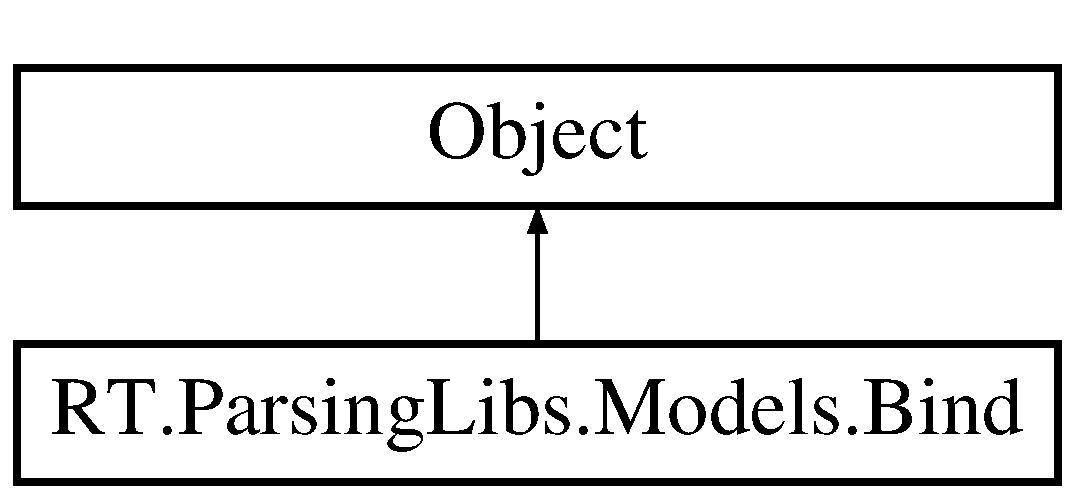
\includegraphics[height=2.000000cm]{class_r_t_1_1_parsing_libs_1_1_models_1_1_bind}
\end{center}
\end{figure}
\subsection*{Открытые члены}
\begin{DoxyCompactItemize}
\item 
\hyperlink{class_r_t_1_1_parsing_libs_1_1_models_1_1_bind_a1f267ab735462ac9086c6f1eec2ebffe}{Bind} ()
\begin{DoxyCompactList}\small\item\em Конструктор по умолчанию \end{DoxyCompactList}\item 
\hyperlink{class_r_t_1_1_parsing_libs_1_1_models_1_1_bind_a982063bf083039d7f1d9704dcd5c86ac}{Bind} (int rubric\+Id, int action\+Id, int region\+Id)
\begin{DoxyCompactList}\small\item\em Конструктор \end{DoxyCompactList}\item 
override string \hyperlink{class_r_t_1_1_parsing_libs_1_1_models_1_1_bind_a822587e1235b85eb9f17ba6b3d634005}{To\+String} ()
\begin{DoxyCompactList}\small\item\em Преобразовать в строку \end{DoxyCompactList}\item 
override bool \hyperlink{class_r_t_1_1_parsing_libs_1_1_models_1_1_bind_a357f6c7991435884fe72b307d893eecf}{Equals} (System.\+Object obj)
\begin{DoxyCompactList}\small\item\em Метод сравнения объектов \end{DoxyCompactList}\item 
bool \hyperlink{class_r_t_1_1_parsing_libs_1_1_models_1_1_bind_aeb1639c9c5370114af8d5413c5f7be33}{Equals} (\hyperlink{class_r_t_1_1_parsing_libs_1_1_models_1_1_bind}{Bind} p)
\begin{DoxyCompactList}\small\item\em Метод сравнения объектов \end{DoxyCompactList}\item 
override int \hyperlink{class_r_t_1_1_parsing_libs_1_1_models_1_1_bind_afcb8edc39a0c01e15aaf51c565d89a00}{Get\+Hash\+Code} ()
\begin{DoxyCompactList}\small\item\em Получить хэш-\/код \end{DoxyCompactList}\end{DoxyCompactItemize}
\subsection*{Свойства}
\begin{DoxyCompactItemize}
\item 
int \hyperlink{class_r_t_1_1_parsing_libs_1_1_models_1_1_bind_a851d2f77b35865675caad8c99d6f4056}{Rubric\+Id}\hspace{0.3cm}{\ttfamily  \mbox{[}get, set\mbox{]}}
\begin{DoxyCompactList}\small\item\em ИД рубрики \end{DoxyCompactList}\item 
int \hyperlink{class_r_t_1_1_parsing_libs_1_1_models_1_1_bind_abee58ed41713f457f61133f58658e933}{Region\+Id}\hspace{0.3cm}{\ttfamily  \mbox{[}get, set\mbox{]}}
\begin{DoxyCompactList}\small\item\em ИД региона \end{DoxyCompactList}\item 
int \hyperlink{class_r_t_1_1_parsing_libs_1_1_models_1_1_bind_a7d8ad0c826c62c743fdceff73d7411a8}{Action\+Id}\hspace{0.3cm}{\ttfamily  \mbox{[}get, set\mbox{]}}
\begin{DoxyCompactList}\small\item\em ИД действия \end{DoxyCompactList}\end{DoxyCompactItemize}


\subsection{Подробное описание}
Бинд (тройка ИД рубрика-\/регион-\/действие) 



\subsection{Конструктор(ы)}
\hypertarget{class_r_t_1_1_parsing_libs_1_1_models_1_1_bind_a1f267ab735462ac9086c6f1eec2ebffe}{\index{R\+T\+::\+Parsing\+Libs\+::\+Models\+::\+Bind@{R\+T\+::\+Parsing\+Libs\+::\+Models\+::\+Bind}!Bind@{Bind}}
\index{Bind@{Bind}!R\+T\+::\+Parsing\+Libs\+::\+Models\+::\+Bind@{R\+T\+::\+Parsing\+Libs\+::\+Models\+::\+Bind}}
\subsubsection[{Bind}]{\setlength{\rightskip}{0pt plus 5cm}R\+T.\+Parsing\+Libs.\+Models.\+Bind.\+Bind (
\begin{DoxyParamCaption}
{}
\end{DoxyParamCaption}
)\hspace{0.3cm}{\ttfamily [inline]}}}\label{class_r_t_1_1_parsing_libs_1_1_models_1_1_bind_a1f267ab735462ac9086c6f1eec2ebffe}


Конструктор по умолчанию 

\hypertarget{class_r_t_1_1_parsing_libs_1_1_models_1_1_bind_a982063bf083039d7f1d9704dcd5c86ac}{\index{R\+T\+::\+Parsing\+Libs\+::\+Models\+::\+Bind@{R\+T\+::\+Parsing\+Libs\+::\+Models\+::\+Bind}!Bind@{Bind}}
\index{Bind@{Bind}!R\+T\+::\+Parsing\+Libs\+::\+Models\+::\+Bind@{R\+T\+::\+Parsing\+Libs\+::\+Models\+::\+Bind}}
\subsubsection[{Bind}]{\setlength{\rightskip}{0pt plus 5cm}R\+T.\+Parsing\+Libs.\+Models.\+Bind.\+Bind (
\begin{DoxyParamCaption}
\item[{int}]{rubric\+Id, }
\item[{int}]{action\+Id, }
\item[{int}]{region\+Id}
\end{DoxyParamCaption}
)\hspace{0.3cm}{\ttfamily [inline]}}}\label{class_r_t_1_1_parsing_libs_1_1_models_1_1_bind_a982063bf083039d7f1d9704dcd5c86ac}


Конструктор 


\begin{DoxyParams}{Аргументы}
{\em rubric\+Id} & ИД рубрики\\
\hline
{\em action\+Id} & ИД действия\\
\hline
{\em region\+Id} & ИД региона\\
\hline
\end{DoxyParams}


\subsection{Методы}
\hypertarget{class_r_t_1_1_parsing_libs_1_1_models_1_1_bind_a357f6c7991435884fe72b307d893eecf}{\index{R\+T\+::\+Parsing\+Libs\+::\+Models\+::\+Bind@{R\+T\+::\+Parsing\+Libs\+::\+Models\+::\+Bind}!Equals@{Equals}}
\index{Equals@{Equals}!R\+T\+::\+Parsing\+Libs\+::\+Models\+::\+Bind@{R\+T\+::\+Parsing\+Libs\+::\+Models\+::\+Bind}}
\subsubsection[{Equals}]{\setlength{\rightskip}{0pt plus 5cm}override bool R\+T.\+Parsing\+Libs.\+Models.\+Bind.\+Equals (
\begin{DoxyParamCaption}
\item[{System.\+Object}]{obj}
\end{DoxyParamCaption}
)\hspace{0.3cm}{\ttfamily [inline]}}}\label{class_r_t_1_1_parsing_libs_1_1_models_1_1_bind_a357f6c7991435884fe72b307d893eecf}


Метод сравнения объектов 


\begin{DoxyParams}{Аргументы}
{\em obj} & Сравниваемый объект\\
\hline
\end{DoxyParams}
\begin{DoxyReturn}{Возвращает}
T\+R\+U\+E -\/ в случае равенства объектов, иначе F\+A\+L\+S\+E
\end{DoxyReturn}
\hypertarget{class_r_t_1_1_parsing_libs_1_1_models_1_1_bind_aeb1639c9c5370114af8d5413c5f7be33}{\index{R\+T\+::\+Parsing\+Libs\+::\+Models\+::\+Bind@{R\+T\+::\+Parsing\+Libs\+::\+Models\+::\+Bind}!Equals@{Equals}}
\index{Equals@{Equals}!R\+T\+::\+Parsing\+Libs\+::\+Models\+::\+Bind@{R\+T\+::\+Parsing\+Libs\+::\+Models\+::\+Bind}}
\subsubsection[{Equals}]{\setlength{\rightskip}{0pt plus 5cm}bool R\+T.\+Parsing\+Libs.\+Models.\+Bind.\+Equals (
\begin{DoxyParamCaption}
\item[{{\bf Bind}}]{p}
\end{DoxyParamCaption}
)\hspace{0.3cm}{\ttfamily [inline]}}}\label{class_r_t_1_1_parsing_libs_1_1_models_1_1_bind_aeb1639c9c5370114af8d5413c5f7be33}


Метод сравнения объектов 


\begin{DoxyParams}{Аргументы}
{\em p} & Сравниваемый объект\\
\hline
\end{DoxyParams}
\begin{DoxyReturn}{Возвращает}
T\+R\+U\+E -\/ в случае равенства объектов, иначе F\+A\+L\+S\+E
\end{DoxyReturn}
\hypertarget{class_r_t_1_1_parsing_libs_1_1_models_1_1_bind_afcb8edc39a0c01e15aaf51c565d89a00}{\index{R\+T\+::\+Parsing\+Libs\+::\+Models\+::\+Bind@{R\+T\+::\+Parsing\+Libs\+::\+Models\+::\+Bind}!Get\+Hash\+Code@{Get\+Hash\+Code}}
\index{Get\+Hash\+Code@{Get\+Hash\+Code}!R\+T\+::\+Parsing\+Libs\+::\+Models\+::\+Bind@{R\+T\+::\+Parsing\+Libs\+::\+Models\+::\+Bind}}
\subsubsection[{Get\+Hash\+Code}]{\setlength{\rightskip}{0pt plus 5cm}override int R\+T.\+Parsing\+Libs.\+Models.\+Bind.\+Get\+Hash\+Code (
\begin{DoxyParamCaption}
{}
\end{DoxyParamCaption}
)\hspace{0.3cm}{\ttfamily [inline]}}}\label{class_r_t_1_1_parsing_libs_1_1_models_1_1_bind_afcb8edc39a0c01e15aaf51c565d89a00}


Получить хэш-\/код 

\begin{DoxyReturn}{Возвращает}
Хэш-\/код
\end{DoxyReturn}
\hypertarget{class_r_t_1_1_parsing_libs_1_1_models_1_1_bind_a822587e1235b85eb9f17ba6b3d634005}{\index{R\+T\+::\+Parsing\+Libs\+::\+Models\+::\+Bind@{R\+T\+::\+Parsing\+Libs\+::\+Models\+::\+Bind}!To\+String@{To\+String}}
\index{To\+String@{To\+String}!R\+T\+::\+Parsing\+Libs\+::\+Models\+::\+Bind@{R\+T\+::\+Parsing\+Libs\+::\+Models\+::\+Bind}}
\subsubsection[{To\+String}]{\setlength{\rightskip}{0pt plus 5cm}override string R\+T.\+Parsing\+Libs.\+Models.\+Bind.\+To\+String (
\begin{DoxyParamCaption}
{}
\end{DoxyParamCaption}
)\hspace{0.3cm}{\ttfamily [inline]}}}\label{class_r_t_1_1_parsing_libs_1_1_models_1_1_bind_a822587e1235b85eb9f17ba6b3d634005}


Преобразовать в строку 

\begin{DoxyReturn}{Возвращает}
Объект в виде строки
\end{DoxyReturn}


\subsection{Полный список свойств}
\hypertarget{class_r_t_1_1_parsing_libs_1_1_models_1_1_bind_a7d8ad0c826c62c743fdceff73d7411a8}{\index{R\+T\+::\+Parsing\+Libs\+::\+Models\+::\+Bind@{R\+T\+::\+Parsing\+Libs\+::\+Models\+::\+Bind}!Action\+Id@{Action\+Id}}
\index{Action\+Id@{Action\+Id}!R\+T\+::\+Parsing\+Libs\+::\+Models\+::\+Bind@{R\+T\+::\+Parsing\+Libs\+::\+Models\+::\+Bind}}
\subsubsection[{Action\+Id}]{\setlength{\rightskip}{0pt plus 5cm}int R\+T.\+Parsing\+Libs.\+Models.\+Bind.\+Action\+Id\hspace{0.3cm}{\ttfamily [get]}, {\ttfamily [set]}}}\label{class_r_t_1_1_parsing_libs_1_1_models_1_1_bind_a7d8ad0c826c62c743fdceff73d7411a8}


ИД действия 

\hypertarget{class_r_t_1_1_parsing_libs_1_1_models_1_1_bind_abee58ed41713f457f61133f58658e933}{\index{R\+T\+::\+Parsing\+Libs\+::\+Models\+::\+Bind@{R\+T\+::\+Parsing\+Libs\+::\+Models\+::\+Bind}!Region\+Id@{Region\+Id}}
\index{Region\+Id@{Region\+Id}!R\+T\+::\+Parsing\+Libs\+::\+Models\+::\+Bind@{R\+T\+::\+Parsing\+Libs\+::\+Models\+::\+Bind}}
\subsubsection[{Region\+Id}]{\setlength{\rightskip}{0pt plus 5cm}int R\+T.\+Parsing\+Libs.\+Models.\+Bind.\+Region\+Id\hspace{0.3cm}{\ttfamily [get]}, {\ttfamily [set]}}}\label{class_r_t_1_1_parsing_libs_1_1_models_1_1_bind_abee58ed41713f457f61133f58658e933}


ИД региона 

\hypertarget{class_r_t_1_1_parsing_libs_1_1_models_1_1_bind_a851d2f77b35865675caad8c99d6f4056}{\index{R\+T\+::\+Parsing\+Libs\+::\+Models\+::\+Bind@{R\+T\+::\+Parsing\+Libs\+::\+Models\+::\+Bind}!Rubric\+Id@{Rubric\+Id}}
\index{Rubric\+Id@{Rubric\+Id}!R\+T\+::\+Parsing\+Libs\+::\+Models\+::\+Bind@{R\+T\+::\+Parsing\+Libs\+::\+Models\+::\+Bind}}
\subsubsection[{Rubric\+Id}]{\setlength{\rightskip}{0pt plus 5cm}int R\+T.\+Parsing\+Libs.\+Models.\+Bind.\+Rubric\+Id\hspace{0.3cm}{\ttfamily [get]}, {\ttfamily [set]}}}\label{class_r_t_1_1_parsing_libs_1_1_models_1_1_bind_a851d2f77b35865675caad8c99d6f4056}


ИД рубрики 



Объявления и описания членов класса находятся в файле\+:\begin{DoxyCompactItemize}
\item 
R\+T.\+Parsing\+Libs/\+Models/Bind.\+cs\end{DoxyCompactItemize}

\hypertarget{class_r_t_1_1_parsing_libs_1_1_models_1_1_namespace_doc}{\section{Класс R\+T.\+Parsing\+Libs.\+Models.\+Namespace\+Doc}
\label{class_r_t_1_1_parsing_libs_1_1_models_1_1_namespace_doc}\index{R\+T.\+Parsing\+Libs.\+Models.\+Namespace\+Doc@{R\+T.\+Parsing\+Libs.\+Models.\+Namespace\+Doc}}
}


\hyperlink{namespace_r_t_1_1_parsing_libs_1_1_models}{R\+T.\+Parsing\+Libs.\+Models} пространство содержит базовые модели для парсеров  




\subsection{Подробное описание}
\hyperlink{namespace_r_t_1_1_parsing_libs_1_1_models}{R\+T.\+Parsing\+Libs.\+Models} пространство содержит базовые модели для парсеров 



Объявления и описания членов класса находятся в файле\+:\begin{DoxyCompactItemize}
\item 
R\+T.\+Parsing\+Libs/\+Models/Namespace\+Doc.\+cs\end{DoxyCompactItemize}

\hypertarget{class_r_t_1_1_parsing_libs_1_1_models_1_1_realty_additional_info}{\section{Класс R\+T.\+Parsing\+Libs.\+Models.\+Realty\+Additional\+Info}
\label{class_r_t_1_1_parsing_libs_1_1_models_1_1_realty_additional_info}\index{R\+T.\+Parsing\+Libs.\+Models.\+Realty\+Additional\+Info@{R\+T.\+Parsing\+Libs.\+Models.\+Realty\+Additional\+Info}}
}


Дополнительная информация для рубрики \char`\"{}Недвижимость\char`\"{}  


\subsection*{Открытые члены}
\begin{DoxyCompactItemize}
\item 
override string \hyperlink{class_r_t_1_1_parsing_libs_1_1_models_1_1_realty_additional_info_ac7f406b43cf8f639cd5f15b148bfed28}{To\+String} ()
\begin{DoxyCompactList}\small\item\em Преобразовать в строку \end{DoxyCompactList}\end{DoxyCompactItemize}
\subsection*{Свойства}
\begin{DoxyCompactItemize}
\item 
int \hyperlink{class_r_t_1_1_parsing_libs_1_1_models_1_1_realty_additional_info_a02f23f31d2d9e8e0364be50880d5ccf0}{Floor\+Number}\hspace{0.3cm}{\ttfamily  \mbox{[}get, set\mbox{]}}
\begin{DoxyCompactList}\small\item\em Количество этажей \end{DoxyCompactList}\item 
int \hyperlink{class_r_t_1_1_parsing_libs_1_1_models_1_1_realty_additional_info_ae907610bd6836056429eff99d7d43d5f}{Floor}\hspace{0.3cm}{\ttfamily  \mbox{[}get, set\mbox{]}}
\begin{DoxyCompactList}\small\item\em Этаж \end{DoxyCompactList}\item 
int \hyperlink{class_r_t_1_1_parsing_libs_1_1_models_1_1_realty_additional_info_a1c6ff9b6b6ea036f2435cb185987e9e8}{Room\+Number}\hspace{0.3cm}{\ttfamily  \mbox{[}get, set\mbox{]}}
\begin{DoxyCompactList}\small\item\em Количество комнат \end{DoxyCompactList}\item 
string \hyperlink{class_r_t_1_1_parsing_libs_1_1_models_1_1_realty_additional_info_a14443c07f02d59130d5a270534e2ebbe}{Real\+Estate\+Type}\hspace{0.3cm}{\ttfamily  \mbox{[}get, set\mbox{]}}
\begin{DoxyCompactList}\small\item\em Тип недвижимости \end{DoxyCompactList}\item 
string \hyperlink{class_r_t_1_1_parsing_libs_1_1_models_1_1_realty_additional_info_a1fec1be576ce133bdcefa6fcae2ea0f8}{District}\hspace{0.3cm}{\ttfamily  \mbox{[}get, set\mbox{]}}
\begin{DoxyCompactList}\small\item\em Район \end{DoxyCompactList}\item 
string \hyperlink{class_r_t_1_1_parsing_libs_1_1_models_1_1_realty_additional_info_a7abbfb44a630c3d2b9d050d26db6a9c4}{Address}\hspace{0.3cm}{\ttfamily  \mbox{[}get, set\mbox{]}}
\begin{DoxyCompactList}\small\item\em Адрес \end{DoxyCompactList}\item 
string \hyperlink{class_r_t_1_1_parsing_libs_1_1_models_1_1_realty_additional_info_a35ff75114c53408faf276711b7cf7b76}{WallМaterial}\hspace{0.3cm}{\ttfamily  \mbox{[}get, set\mbox{]}}
\begin{DoxyCompactList}\small\item\em Материал стен \end{DoxyCompactList}\item 
string \hyperlink{class_r_t_1_1_parsing_libs_1_1_models_1_1_realty_additional_info_a21d62bfc34bfac813226b73967e52dd0}{Furnish}\hspace{0.3cm}{\ttfamily  \mbox{[}get, set\mbox{]}}
\begin{DoxyCompactList}\small\item\em Отделка \end{DoxyCompactList}\item 
int \hyperlink{class_r_t_1_1_parsing_libs_1_1_models_1_1_realty_additional_info_a00613206f5cfd14f14eb11a348b0546f}{Total\+Space}\hspace{0.3cm}{\ttfamily  \mbox{[}get, set\mbox{]}}
\begin{DoxyCompactList}\small\item\em Общая площадь \end{DoxyCompactList}\item 
int \hyperlink{class_r_t_1_1_parsing_libs_1_1_models_1_1_realty_additional_info_ab0fdc5195b608faf8b0be3ac47a2266b}{Living\+Space}\hspace{0.3cm}{\ttfamily  \mbox{[}get, set\mbox{]}}
\begin{DoxyCompactList}\small\item\em Жилая площадь \end{DoxyCompactList}\item 
int \hyperlink{class_r_t_1_1_parsing_libs_1_1_models_1_1_realty_additional_info_a6dd7cad405e1fdbd63f7ba51bd9382bb}{Kitchen\+Space}\hspace{0.3cm}{\ttfamily  \mbox{[}get, set\mbox{]}}
\begin{DoxyCompactList}\small\item\em Площадь кухни \end{DoxyCompactList}\item 
decimal \hyperlink{class_r_t_1_1_parsing_libs_1_1_models_1_1_realty_additional_info_a71237b220ed87f13f18d71975436c9a2}{Cost\+All}\hspace{0.3cm}{\ttfamily  \mbox{[}get, set\mbox{]}}
\begin{DoxyCompactList}\small\item\em Цена за весь объект \end{DoxyCompactList}\item 
decimal \hyperlink{class_r_t_1_1_parsing_libs_1_1_models_1_1_realty_additional_info_a748d3e4584bfcbfb157781497f27c5ab}{Cost\+Per\+Meter}\hspace{0.3cm}{\ttfamily  \mbox{[}get, set\mbox{]}}
\begin{DoxyCompactList}\small\item\em Цена за метр \end{DoxyCompactList}\item 
bool \hyperlink{class_r_t_1_1_parsing_libs_1_1_models_1_1_realty_additional_info_adc0122a3b59b56c2231c5c06f1245f22}{Is\+Loggia}\hspace{0.3cm}{\ttfamily  \mbox{[}get, set\mbox{]}}
\begin{DoxyCompactList}\small\item\em Балкон/лоджия \end{DoxyCompactList}\item 
string \hyperlink{class_r_t_1_1_parsing_libs_1_1_models_1_1_realty_additional_info_aedcbc8e48fa63f3705c88bf73ed4a265}{Wc}\hspace{0.3cm}{\ttfamily  \mbox{[}get, set\mbox{]}}
\begin{DoxyCompactList}\small\item\em Санузел \end{DoxyCompactList}\item 
string \hyperlink{class_r_t_1_1_parsing_libs_1_1_models_1_1_realty_additional_info_a631100f22c2651ccb17c279fa3eee358}{View\+From\+Property}\hspace{0.3cm}{\ttfamily  \mbox{[}get, set\mbox{]}}
\begin{DoxyCompactList}\small\item\em Вид из окон \end{DoxyCompactList}\item 
bool \hyperlink{class_r_t_1_1_parsing_libs_1_1_models_1_1_realty_additional_info_afe747cb54823715884003f2440b95f16}{Is\+Parking}\hspace{0.3cm}{\ttfamily  \mbox{[}get, set\mbox{]}}
\begin{DoxyCompactList}\small\item\em Паркинг во дворе или доме \end{DoxyCompactList}\item 
int \hyperlink{class_r_t_1_1_parsing_libs_1_1_models_1_1_realty_additional_info_a1e175c5a4c34af76b575b7b640d189a9}{Tenancy}\hspace{0.3cm}{\ttfamily  \mbox{[}get, set\mbox{]}}
\begin{DoxyCompactList}\small\item\em Срок аренды \end{DoxyCompactList}\item 
int \hyperlink{class_r_t_1_1_parsing_libs_1_1_models_1_1_realty_additional_info_a2b5232cd91f9e28df8cd7619e2686af2}{Leasable\+Space}\hspace{0.3cm}{\ttfamily  \mbox{[}get, set\mbox{]}}
\begin{DoxyCompactList}\small\item\em Сдаваемая площадь \end{DoxyCompactList}\item 
string \hyperlink{class_r_t_1_1_parsing_libs_1_1_models_1_1_realty_additional_info_ae3401a05dd43d8afbda00fffc5b16b78}{Appointment\+Of\+Room}\hspace{0.3cm}{\ttfamily  \mbox{[}get, set\mbox{]}}
\begin{DoxyCompactList}\small\item\em Назначение помещения \end{DoxyCompactList}\item 
int \hyperlink{class_r_t_1_1_parsing_libs_1_1_models_1_1_realty_additional_info_a803bc8536454d7d89bfb72878767e7cb}{Land\+Space}\hspace{0.3cm}{\ttfamily  \mbox{[}get, set\mbox{]}}
\begin{DoxyCompactList}\small\item\em Площадь участка, соток \end{DoxyCompactList}\end{DoxyCompactItemize}


\subsection{Подробное описание}
Дополнительная информация для рубрики \char`\"{}Недвижимость\char`\"{} 



\subsection{Методы}
\hypertarget{class_r_t_1_1_parsing_libs_1_1_models_1_1_realty_additional_info_ac7f406b43cf8f639cd5f15b148bfed28}{\index{R\+T\+::\+Parsing\+Libs\+::\+Models\+::\+Realty\+Additional\+Info@{R\+T\+::\+Parsing\+Libs\+::\+Models\+::\+Realty\+Additional\+Info}!To\+String@{To\+String}}
\index{To\+String@{To\+String}!R\+T\+::\+Parsing\+Libs\+::\+Models\+::\+Realty\+Additional\+Info@{R\+T\+::\+Parsing\+Libs\+::\+Models\+::\+Realty\+Additional\+Info}}
\subsubsection[{To\+String}]{\setlength{\rightskip}{0pt plus 5cm}override string R\+T.\+Parsing\+Libs.\+Models.\+Realty\+Additional\+Info.\+To\+String (
\begin{DoxyParamCaption}
{}
\end{DoxyParamCaption}
)\hspace{0.3cm}{\ttfamily [inline]}}}\label{class_r_t_1_1_parsing_libs_1_1_models_1_1_realty_additional_info_ac7f406b43cf8f639cd5f15b148bfed28}


Преобразовать в строку 

\begin{DoxyReturn}{Возвращает}
Объект в виде строки
\end{DoxyReturn}


\subsection{Полный список свойств}
\hypertarget{class_r_t_1_1_parsing_libs_1_1_models_1_1_realty_additional_info_a7abbfb44a630c3d2b9d050d26db6a9c4}{\index{R\+T\+::\+Parsing\+Libs\+::\+Models\+::\+Realty\+Additional\+Info@{R\+T\+::\+Parsing\+Libs\+::\+Models\+::\+Realty\+Additional\+Info}!Address@{Address}}
\index{Address@{Address}!R\+T\+::\+Parsing\+Libs\+::\+Models\+::\+Realty\+Additional\+Info@{R\+T\+::\+Parsing\+Libs\+::\+Models\+::\+Realty\+Additional\+Info}}
\subsubsection[{Address}]{\setlength{\rightskip}{0pt plus 5cm}string R\+T.\+Parsing\+Libs.\+Models.\+Realty\+Additional\+Info.\+Address\hspace{0.3cm}{\ttfamily [get]}, {\ttfamily [set]}}}\label{class_r_t_1_1_parsing_libs_1_1_models_1_1_realty_additional_info_a7abbfb44a630c3d2b9d050d26db6a9c4}


Адрес 

\hypertarget{class_r_t_1_1_parsing_libs_1_1_models_1_1_realty_additional_info_ae3401a05dd43d8afbda00fffc5b16b78}{\index{R\+T\+::\+Parsing\+Libs\+::\+Models\+::\+Realty\+Additional\+Info@{R\+T\+::\+Parsing\+Libs\+::\+Models\+::\+Realty\+Additional\+Info}!Appointment\+Of\+Room@{Appointment\+Of\+Room}}
\index{Appointment\+Of\+Room@{Appointment\+Of\+Room}!R\+T\+::\+Parsing\+Libs\+::\+Models\+::\+Realty\+Additional\+Info@{R\+T\+::\+Parsing\+Libs\+::\+Models\+::\+Realty\+Additional\+Info}}
\subsubsection[{Appointment\+Of\+Room}]{\setlength{\rightskip}{0pt plus 5cm}string R\+T.\+Parsing\+Libs.\+Models.\+Realty\+Additional\+Info.\+Appointment\+Of\+Room\hspace{0.3cm}{\ttfamily [get]}, {\ttfamily [set]}}}\label{class_r_t_1_1_parsing_libs_1_1_models_1_1_realty_additional_info_ae3401a05dd43d8afbda00fffc5b16b78}


Назначение помещения 

\hypertarget{class_r_t_1_1_parsing_libs_1_1_models_1_1_realty_additional_info_a71237b220ed87f13f18d71975436c9a2}{\index{R\+T\+::\+Parsing\+Libs\+::\+Models\+::\+Realty\+Additional\+Info@{R\+T\+::\+Parsing\+Libs\+::\+Models\+::\+Realty\+Additional\+Info}!Cost\+All@{Cost\+All}}
\index{Cost\+All@{Cost\+All}!R\+T\+::\+Parsing\+Libs\+::\+Models\+::\+Realty\+Additional\+Info@{R\+T\+::\+Parsing\+Libs\+::\+Models\+::\+Realty\+Additional\+Info}}
\subsubsection[{Cost\+All}]{\setlength{\rightskip}{0pt plus 5cm}decimal R\+T.\+Parsing\+Libs.\+Models.\+Realty\+Additional\+Info.\+Cost\+All\hspace{0.3cm}{\ttfamily [get]}, {\ttfamily [set]}}}\label{class_r_t_1_1_parsing_libs_1_1_models_1_1_realty_additional_info_a71237b220ed87f13f18d71975436c9a2}


Цена за весь объект 

\hypertarget{class_r_t_1_1_parsing_libs_1_1_models_1_1_realty_additional_info_a748d3e4584bfcbfb157781497f27c5ab}{\index{R\+T\+::\+Parsing\+Libs\+::\+Models\+::\+Realty\+Additional\+Info@{R\+T\+::\+Parsing\+Libs\+::\+Models\+::\+Realty\+Additional\+Info}!Cost\+Per\+Meter@{Cost\+Per\+Meter}}
\index{Cost\+Per\+Meter@{Cost\+Per\+Meter}!R\+T\+::\+Parsing\+Libs\+::\+Models\+::\+Realty\+Additional\+Info@{R\+T\+::\+Parsing\+Libs\+::\+Models\+::\+Realty\+Additional\+Info}}
\subsubsection[{Cost\+Per\+Meter}]{\setlength{\rightskip}{0pt plus 5cm}decimal R\+T.\+Parsing\+Libs.\+Models.\+Realty\+Additional\+Info.\+Cost\+Per\+Meter\hspace{0.3cm}{\ttfamily [get]}, {\ttfamily [set]}}}\label{class_r_t_1_1_parsing_libs_1_1_models_1_1_realty_additional_info_a748d3e4584bfcbfb157781497f27c5ab}


Цена за метр 

\hypertarget{class_r_t_1_1_parsing_libs_1_1_models_1_1_realty_additional_info_a1fec1be576ce133bdcefa6fcae2ea0f8}{\index{R\+T\+::\+Parsing\+Libs\+::\+Models\+::\+Realty\+Additional\+Info@{R\+T\+::\+Parsing\+Libs\+::\+Models\+::\+Realty\+Additional\+Info}!District@{District}}
\index{District@{District}!R\+T\+::\+Parsing\+Libs\+::\+Models\+::\+Realty\+Additional\+Info@{R\+T\+::\+Parsing\+Libs\+::\+Models\+::\+Realty\+Additional\+Info}}
\subsubsection[{District}]{\setlength{\rightskip}{0pt plus 5cm}string R\+T.\+Parsing\+Libs.\+Models.\+Realty\+Additional\+Info.\+District\hspace{0.3cm}{\ttfamily [get]}, {\ttfamily [set]}}}\label{class_r_t_1_1_parsing_libs_1_1_models_1_1_realty_additional_info_a1fec1be576ce133bdcefa6fcae2ea0f8}


Район 

\hypertarget{class_r_t_1_1_parsing_libs_1_1_models_1_1_realty_additional_info_ae907610bd6836056429eff99d7d43d5f}{\index{R\+T\+::\+Parsing\+Libs\+::\+Models\+::\+Realty\+Additional\+Info@{R\+T\+::\+Parsing\+Libs\+::\+Models\+::\+Realty\+Additional\+Info}!Floor@{Floor}}
\index{Floor@{Floor}!R\+T\+::\+Parsing\+Libs\+::\+Models\+::\+Realty\+Additional\+Info@{R\+T\+::\+Parsing\+Libs\+::\+Models\+::\+Realty\+Additional\+Info}}
\subsubsection[{Floor}]{\setlength{\rightskip}{0pt plus 5cm}int R\+T.\+Parsing\+Libs.\+Models.\+Realty\+Additional\+Info.\+Floor\hspace{0.3cm}{\ttfamily [get]}, {\ttfamily [set]}}}\label{class_r_t_1_1_parsing_libs_1_1_models_1_1_realty_additional_info_ae907610bd6836056429eff99d7d43d5f}


Этаж 

\hypertarget{class_r_t_1_1_parsing_libs_1_1_models_1_1_realty_additional_info_a02f23f31d2d9e8e0364be50880d5ccf0}{\index{R\+T\+::\+Parsing\+Libs\+::\+Models\+::\+Realty\+Additional\+Info@{R\+T\+::\+Parsing\+Libs\+::\+Models\+::\+Realty\+Additional\+Info}!Floor\+Number@{Floor\+Number}}
\index{Floor\+Number@{Floor\+Number}!R\+T\+::\+Parsing\+Libs\+::\+Models\+::\+Realty\+Additional\+Info@{R\+T\+::\+Parsing\+Libs\+::\+Models\+::\+Realty\+Additional\+Info}}
\subsubsection[{Floor\+Number}]{\setlength{\rightskip}{0pt plus 5cm}int R\+T.\+Parsing\+Libs.\+Models.\+Realty\+Additional\+Info.\+Floor\+Number\hspace{0.3cm}{\ttfamily [get]}, {\ttfamily [set]}}}\label{class_r_t_1_1_parsing_libs_1_1_models_1_1_realty_additional_info_a02f23f31d2d9e8e0364be50880d5ccf0}


Количество этажей 

\hypertarget{class_r_t_1_1_parsing_libs_1_1_models_1_1_realty_additional_info_a21d62bfc34bfac813226b73967e52dd0}{\index{R\+T\+::\+Parsing\+Libs\+::\+Models\+::\+Realty\+Additional\+Info@{R\+T\+::\+Parsing\+Libs\+::\+Models\+::\+Realty\+Additional\+Info}!Furnish@{Furnish}}
\index{Furnish@{Furnish}!R\+T\+::\+Parsing\+Libs\+::\+Models\+::\+Realty\+Additional\+Info@{R\+T\+::\+Parsing\+Libs\+::\+Models\+::\+Realty\+Additional\+Info}}
\subsubsection[{Furnish}]{\setlength{\rightskip}{0pt plus 5cm}string R\+T.\+Parsing\+Libs.\+Models.\+Realty\+Additional\+Info.\+Furnish\hspace{0.3cm}{\ttfamily [get]}, {\ttfamily [set]}}}\label{class_r_t_1_1_parsing_libs_1_1_models_1_1_realty_additional_info_a21d62bfc34bfac813226b73967e52dd0}


Отделка 

\hypertarget{class_r_t_1_1_parsing_libs_1_1_models_1_1_realty_additional_info_adc0122a3b59b56c2231c5c06f1245f22}{\index{R\+T\+::\+Parsing\+Libs\+::\+Models\+::\+Realty\+Additional\+Info@{R\+T\+::\+Parsing\+Libs\+::\+Models\+::\+Realty\+Additional\+Info}!Is\+Loggia@{Is\+Loggia}}
\index{Is\+Loggia@{Is\+Loggia}!R\+T\+::\+Parsing\+Libs\+::\+Models\+::\+Realty\+Additional\+Info@{R\+T\+::\+Parsing\+Libs\+::\+Models\+::\+Realty\+Additional\+Info}}
\subsubsection[{Is\+Loggia}]{\setlength{\rightskip}{0pt plus 5cm}bool R\+T.\+Parsing\+Libs.\+Models.\+Realty\+Additional\+Info.\+Is\+Loggia\hspace{0.3cm}{\ttfamily [get]}, {\ttfamily [set]}}}\label{class_r_t_1_1_parsing_libs_1_1_models_1_1_realty_additional_info_adc0122a3b59b56c2231c5c06f1245f22}


Балкон/лоджия 

\hypertarget{class_r_t_1_1_parsing_libs_1_1_models_1_1_realty_additional_info_afe747cb54823715884003f2440b95f16}{\index{R\+T\+::\+Parsing\+Libs\+::\+Models\+::\+Realty\+Additional\+Info@{R\+T\+::\+Parsing\+Libs\+::\+Models\+::\+Realty\+Additional\+Info}!Is\+Parking@{Is\+Parking}}
\index{Is\+Parking@{Is\+Parking}!R\+T\+::\+Parsing\+Libs\+::\+Models\+::\+Realty\+Additional\+Info@{R\+T\+::\+Parsing\+Libs\+::\+Models\+::\+Realty\+Additional\+Info}}
\subsubsection[{Is\+Parking}]{\setlength{\rightskip}{0pt plus 5cm}bool R\+T.\+Parsing\+Libs.\+Models.\+Realty\+Additional\+Info.\+Is\+Parking\hspace{0.3cm}{\ttfamily [get]}, {\ttfamily [set]}}}\label{class_r_t_1_1_parsing_libs_1_1_models_1_1_realty_additional_info_afe747cb54823715884003f2440b95f16}


Паркинг во дворе или доме 

\hypertarget{class_r_t_1_1_parsing_libs_1_1_models_1_1_realty_additional_info_a6dd7cad405e1fdbd63f7ba51bd9382bb}{\index{R\+T\+::\+Parsing\+Libs\+::\+Models\+::\+Realty\+Additional\+Info@{R\+T\+::\+Parsing\+Libs\+::\+Models\+::\+Realty\+Additional\+Info}!Kitchen\+Space@{Kitchen\+Space}}
\index{Kitchen\+Space@{Kitchen\+Space}!R\+T\+::\+Parsing\+Libs\+::\+Models\+::\+Realty\+Additional\+Info@{R\+T\+::\+Parsing\+Libs\+::\+Models\+::\+Realty\+Additional\+Info}}
\subsubsection[{Kitchen\+Space}]{\setlength{\rightskip}{0pt plus 5cm}int R\+T.\+Parsing\+Libs.\+Models.\+Realty\+Additional\+Info.\+Kitchen\+Space\hspace{0.3cm}{\ttfamily [get]}, {\ttfamily [set]}}}\label{class_r_t_1_1_parsing_libs_1_1_models_1_1_realty_additional_info_a6dd7cad405e1fdbd63f7ba51bd9382bb}


Площадь кухни 

\hypertarget{class_r_t_1_1_parsing_libs_1_1_models_1_1_realty_additional_info_a803bc8536454d7d89bfb72878767e7cb}{\index{R\+T\+::\+Parsing\+Libs\+::\+Models\+::\+Realty\+Additional\+Info@{R\+T\+::\+Parsing\+Libs\+::\+Models\+::\+Realty\+Additional\+Info}!Land\+Space@{Land\+Space}}
\index{Land\+Space@{Land\+Space}!R\+T\+::\+Parsing\+Libs\+::\+Models\+::\+Realty\+Additional\+Info@{R\+T\+::\+Parsing\+Libs\+::\+Models\+::\+Realty\+Additional\+Info}}
\subsubsection[{Land\+Space}]{\setlength{\rightskip}{0pt plus 5cm}int R\+T.\+Parsing\+Libs.\+Models.\+Realty\+Additional\+Info.\+Land\+Space\hspace{0.3cm}{\ttfamily [get]}, {\ttfamily [set]}}}\label{class_r_t_1_1_parsing_libs_1_1_models_1_1_realty_additional_info_a803bc8536454d7d89bfb72878767e7cb}


Площадь участка, соток 

\hypertarget{class_r_t_1_1_parsing_libs_1_1_models_1_1_realty_additional_info_a2b5232cd91f9e28df8cd7619e2686af2}{\index{R\+T\+::\+Parsing\+Libs\+::\+Models\+::\+Realty\+Additional\+Info@{R\+T\+::\+Parsing\+Libs\+::\+Models\+::\+Realty\+Additional\+Info}!Leasable\+Space@{Leasable\+Space}}
\index{Leasable\+Space@{Leasable\+Space}!R\+T\+::\+Parsing\+Libs\+::\+Models\+::\+Realty\+Additional\+Info@{R\+T\+::\+Parsing\+Libs\+::\+Models\+::\+Realty\+Additional\+Info}}
\subsubsection[{Leasable\+Space}]{\setlength{\rightskip}{0pt plus 5cm}int R\+T.\+Parsing\+Libs.\+Models.\+Realty\+Additional\+Info.\+Leasable\+Space\hspace{0.3cm}{\ttfamily [get]}, {\ttfamily [set]}}}\label{class_r_t_1_1_parsing_libs_1_1_models_1_1_realty_additional_info_a2b5232cd91f9e28df8cd7619e2686af2}


Сдаваемая площадь 

\hypertarget{class_r_t_1_1_parsing_libs_1_1_models_1_1_realty_additional_info_ab0fdc5195b608faf8b0be3ac47a2266b}{\index{R\+T\+::\+Parsing\+Libs\+::\+Models\+::\+Realty\+Additional\+Info@{R\+T\+::\+Parsing\+Libs\+::\+Models\+::\+Realty\+Additional\+Info}!Living\+Space@{Living\+Space}}
\index{Living\+Space@{Living\+Space}!R\+T\+::\+Parsing\+Libs\+::\+Models\+::\+Realty\+Additional\+Info@{R\+T\+::\+Parsing\+Libs\+::\+Models\+::\+Realty\+Additional\+Info}}
\subsubsection[{Living\+Space}]{\setlength{\rightskip}{0pt plus 5cm}int R\+T.\+Parsing\+Libs.\+Models.\+Realty\+Additional\+Info.\+Living\+Space\hspace{0.3cm}{\ttfamily [get]}, {\ttfamily [set]}}}\label{class_r_t_1_1_parsing_libs_1_1_models_1_1_realty_additional_info_ab0fdc5195b608faf8b0be3ac47a2266b}


Жилая площадь 

\hypertarget{class_r_t_1_1_parsing_libs_1_1_models_1_1_realty_additional_info_a14443c07f02d59130d5a270534e2ebbe}{\index{R\+T\+::\+Parsing\+Libs\+::\+Models\+::\+Realty\+Additional\+Info@{R\+T\+::\+Parsing\+Libs\+::\+Models\+::\+Realty\+Additional\+Info}!Real\+Estate\+Type@{Real\+Estate\+Type}}
\index{Real\+Estate\+Type@{Real\+Estate\+Type}!R\+T\+::\+Parsing\+Libs\+::\+Models\+::\+Realty\+Additional\+Info@{R\+T\+::\+Parsing\+Libs\+::\+Models\+::\+Realty\+Additional\+Info}}
\subsubsection[{Real\+Estate\+Type}]{\setlength{\rightskip}{0pt plus 5cm}string R\+T.\+Parsing\+Libs.\+Models.\+Realty\+Additional\+Info.\+Real\+Estate\+Type\hspace{0.3cm}{\ttfamily [get]}, {\ttfamily [set]}}}\label{class_r_t_1_1_parsing_libs_1_1_models_1_1_realty_additional_info_a14443c07f02d59130d5a270534e2ebbe}


Тип недвижимости 

\hypertarget{class_r_t_1_1_parsing_libs_1_1_models_1_1_realty_additional_info_a1c6ff9b6b6ea036f2435cb185987e9e8}{\index{R\+T\+::\+Parsing\+Libs\+::\+Models\+::\+Realty\+Additional\+Info@{R\+T\+::\+Parsing\+Libs\+::\+Models\+::\+Realty\+Additional\+Info}!Room\+Number@{Room\+Number}}
\index{Room\+Number@{Room\+Number}!R\+T\+::\+Parsing\+Libs\+::\+Models\+::\+Realty\+Additional\+Info@{R\+T\+::\+Parsing\+Libs\+::\+Models\+::\+Realty\+Additional\+Info}}
\subsubsection[{Room\+Number}]{\setlength{\rightskip}{0pt plus 5cm}int R\+T.\+Parsing\+Libs.\+Models.\+Realty\+Additional\+Info.\+Room\+Number\hspace{0.3cm}{\ttfamily [get]}, {\ttfamily [set]}}}\label{class_r_t_1_1_parsing_libs_1_1_models_1_1_realty_additional_info_a1c6ff9b6b6ea036f2435cb185987e9e8}


Количество комнат 

\hypertarget{class_r_t_1_1_parsing_libs_1_1_models_1_1_realty_additional_info_a1e175c5a4c34af76b575b7b640d189a9}{\index{R\+T\+::\+Parsing\+Libs\+::\+Models\+::\+Realty\+Additional\+Info@{R\+T\+::\+Parsing\+Libs\+::\+Models\+::\+Realty\+Additional\+Info}!Tenancy@{Tenancy}}
\index{Tenancy@{Tenancy}!R\+T\+::\+Parsing\+Libs\+::\+Models\+::\+Realty\+Additional\+Info@{R\+T\+::\+Parsing\+Libs\+::\+Models\+::\+Realty\+Additional\+Info}}
\subsubsection[{Tenancy}]{\setlength{\rightskip}{0pt plus 5cm}int R\+T.\+Parsing\+Libs.\+Models.\+Realty\+Additional\+Info.\+Tenancy\hspace{0.3cm}{\ttfamily [get]}, {\ttfamily [set]}}}\label{class_r_t_1_1_parsing_libs_1_1_models_1_1_realty_additional_info_a1e175c5a4c34af76b575b7b640d189a9}


Срок аренды 

\hypertarget{class_r_t_1_1_parsing_libs_1_1_models_1_1_realty_additional_info_a00613206f5cfd14f14eb11a348b0546f}{\index{R\+T\+::\+Parsing\+Libs\+::\+Models\+::\+Realty\+Additional\+Info@{R\+T\+::\+Parsing\+Libs\+::\+Models\+::\+Realty\+Additional\+Info}!Total\+Space@{Total\+Space}}
\index{Total\+Space@{Total\+Space}!R\+T\+::\+Parsing\+Libs\+::\+Models\+::\+Realty\+Additional\+Info@{R\+T\+::\+Parsing\+Libs\+::\+Models\+::\+Realty\+Additional\+Info}}
\subsubsection[{Total\+Space}]{\setlength{\rightskip}{0pt plus 5cm}int R\+T.\+Parsing\+Libs.\+Models.\+Realty\+Additional\+Info.\+Total\+Space\hspace{0.3cm}{\ttfamily [get]}, {\ttfamily [set]}}}\label{class_r_t_1_1_parsing_libs_1_1_models_1_1_realty_additional_info_a00613206f5cfd14f14eb11a348b0546f}


Общая площадь 

\hypertarget{class_r_t_1_1_parsing_libs_1_1_models_1_1_realty_additional_info_a631100f22c2651ccb17c279fa3eee358}{\index{R\+T\+::\+Parsing\+Libs\+::\+Models\+::\+Realty\+Additional\+Info@{R\+T\+::\+Parsing\+Libs\+::\+Models\+::\+Realty\+Additional\+Info}!View\+From\+Property@{View\+From\+Property}}
\index{View\+From\+Property@{View\+From\+Property}!R\+T\+::\+Parsing\+Libs\+::\+Models\+::\+Realty\+Additional\+Info@{R\+T\+::\+Parsing\+Libs\+::\+Models\+::\+Realty\+Additional\+Info}}
\subsubsection[{View\+From\+Property}]{\setlength{\rightskip}{0pt plus 5cm}string R\+T.\+Parsing\+Libs.\+Models.\+Realty\+Additional\+Info.\+View\+From\+Property\hspace{0.3cm}{\ttfamily [get]}, {\ttfamily [set]}}}\label{class_r_t_1_1_parsing_libs_1_1_models_1_1_realty_additional_info_a631100f22c2651ccb17c279fa3eee358}


Вид из окон 

\hypertarget{class_r_t_1_1_parsing_libs_1_1_models_1_1_realty_additional_info_a35ff75114c53408faf276711b7cf7b76}{\index{R\+T\+::\+Parsing\+Libs\+::\+Models\+::\+Realty\+Additional\+Info@{R\+T\+::\+Parsing\+Libs\+::\+Models\+::\+Realty\+Additional\+Info}!WallМaterial@{WallМaterial}}
\index{WallМaterial@{WallМaterial}!R\+T\+::\+Parsing\+Libs\+::\+Models\+::\+Realty\+Additional\+Info@{R\+T\+::\+Parsing\+Libs\+::\+Models\+::\+Realty\+Additional\+Info}}
\subsubsection[{WallМaterial}]{\setlength{\rightskip}{0pt plus 5cm}string R\+T.\+Parsing\+Libs.\+Models.\+Realty\+Additional\+Info.\+WallМaterial\hspace{0.3cm}{\ttfamily [get]}, {\ttfamily [set]}}}\label{class_r_t_1_1_parsing_libs_1_1_models_1_1_realty_additional_info_a35ff75114c53408faf276711b7cf7b76}


Материал стен 

\hypertarget{class_r_t_1_1_parsing_libs_1_1_models_1_1_realty_additional_info_aedcbc8e48fa63f3705c88bf73ed4a265}{\index{R\+T\+::\+Parsing\+Libs\+::\+Models\+::\+Realty\+Additional\+Info@{R\+T\+::\+Parsing\+Libs\+::\+Models\+::\+Realty\+Additional\+Info}!Wc@{Wc}}
\index{Wc@{Wc}!R\+T\+::\+Parsing\+Libs\+::\+Models\+::\+Realty\+Additional\+Info@{R\+T\+::\+Parsing\+Libs\+::\+Models\+::\+Realty\+Additional\+Info}}
\subsubsection[{Wc}]{\setlength{\rightskip}{0pt plus 5cm}string R\+T.\+Parsing\+Libs.\+Models.\+Realty\+Additional\+Info.\+Wc\hspace{0.3cm}{\ttfamily [get]}, {\ttfamily [set]}}}\label{class_r_t_1_1_parsing_libs_1_1_models_1_1_realty_additional_info_aedcbc8e48fa63f3705c88bf73ed4a265}


Санузел 



Объявления и описания членов класса находятся в файле\+:\begin{DoxyCompactItemize}
\item 
R\+T.\+Parsing\+Libs/\+Models/Realty\+Additional\+Info.\+cs\end{DoxyCompactItemize}

\hypertarget{class_r_t_1_1_parsing_libs_1_1_models_1_1_web_publication}{\section{Класс R\+T.\+Parsing\+Libs.\+Models.\+Web\+Publication}
\label{class_r_t_1_1_parsing_libs_1_1_models_1_1_web_publication}\index{R\+T.\+Parsing\+Libs.\+Models.\+Web\+Publication@{R\+T.\+Parsing\+Libs.\+Models.\+Web\+Publication}}
}


Объявление  


\subsection*{Открытые члены}
\begin{DoxyCompactItemize}
\item 
override string \hyperlink{class_r_t_1_1_parsing_libs_1_1_models_1_1_web_publication_a80d88cd1f8ff7cbdf496a5fec5a879bf}{To\+String} ()
\begin{DoxyCompactList}\small\item\em Преобразовать в строку \end{DoxyCompactList}\end{DoxyCompactItemize}
\subsection*{Свойства}
\begin{DoxyCompactItemize}
\item 
string \hyperlink{class_r_t_1_1_parsing_libs_1_1_models_1_1_web_publication_ae9aa1c3f6b51812ca50dd0b389927a6a}{Publication\+Id}\hspace{0.3cm}{\ttfamily  \mbox{[}get, set\mbox{]}}
\begin{DoxyCompactList}\small\item\em ИД объявления в данной рубрике-\/регионе-\/дествии \end{DoxyCompactList}\item 
Date\+Time \hyperlink{class_r_t_1_1_parsing_libs_1_1_models_1_1_web_publication_a34bc37b2cb2fdec3aa98c2a9dc934821}{Modify\+Date}\hspace{0.3cm}{\ttfamily  \mbox{[}get, set\mbox{]}}
\begin{DoxyCompactList}\small\item\em Дата создания/изменения объявления \end{DoxyCompactList}\item 
long \hyperlink{class_r_t_1_1_parsing_libs_1_1_models_1_1_web_publication_a08cca4867a7785ad2c65ea69d912b8fb}{Rubric\+Id}\hspace{0.3cm}{\ttfamily  \mbox{[}get, set\mbox{]}}
\begin{DoxyCompactList}\small\item\em ИД рубрики \end{DoxyCompactList}\item 
long \hyperlink{class_r_t_1_1_parsing_libs_1_1_models_1_1_web_publication_ac617cee04f4c38b132e27c19d375bf54}{Region\+Id}\hspace{0.3cm}{\ttfamily  \mbox{[}get, set\mbox{]}}
\begin{DoxyCompactList}\small\item\em ИД региона \end{DoxyCompactList}\item 
long \hyperlink{class_r_t_1_1_parsing_libs_1_1_models_1_1_web_publication_ae9b9c8570cb37cfe1941bdcf13a723f6}{Action\+Id}\hspace{0.3cm}{\ttfamily  \mbox{[}get, set\mbox{]}}
\begin{DoxyCompactList}\small\item\em ИД действия \end{DoxyCompactList}\item 
Uri \hyperlink{class_r_t_1_1_parsing_libs_1_1_models_1_1_web_publication_a0454089a5089f84a07ab7319af913ad1}{Url}\hspace{0.3cm}{\ttfamily  \mbox{[}get, set\mbox{]}}
\begin{DoxyCompactList}\small\item\em Ссылка на объявление \end{DoxyCompactList}\item 
Uri \hyperlink{class_r_t_1_1_parsing_libs_1_1_models_1_1_web_publication_ac9d070259cf5f0f2beb25a4cd9596531}{Site}\hspace{0.3cm}{\ttfamily  \mbox{[}get, set\mbox{]}}
\begin{DoxyCompactList}\small\item\em Ссылка на сайт \end{DoxyCompactList}\item 
string \hyperlink{class_r_t_1_1_parsing_libs_1_1_models_1_1_web_publication_a7e4f6b52fd3540c2b1a53d5371f82165}{Description}\hspace{0.3cm}{\ttfamily  \mbox{[}get, set\mbox{]}}
\begin{DoxyCompactList}\small\item\em Текст объявления \end{DoxyCompactList}\item 
\hyperlink{class_r_t_1_1_parsing_libs_1_1_models_1_1_web_publication_contact}{Web\+Publication\+Contact} \hyperlink{class_r_t_1_1_parsing_libs_1_1_models_1_1_web_publication_a34ef01cdaf0cf3f46daf5cecb67e2013}{Contact}\hspace{0.3cm}{\ttfamily  \mbox{[}get, set\mbox{]}}
\begin{DoxyCompactList}\small\item\em Контакт объявления \end{DoxyCompactList}\item 
I\+List$<$ Uri $>$ \hyperlink{class_r_t_1_1_parsing_libs_1_1_models_1_1_web_publication_a01108884b89ec964466b0db8c187d031}{Photos}\hspace{0.3cm}{\ttfamily  \mbox{[}get, set\mbox{]}}
\begin{DoxyCompactList}\small\item\em Url на изображения \end{DoxyCompactList}\item 
\hyperlink{class_r_t_1_1_parsing_libs_1_1_models_1_1_additional_info}{Additional\+Info} \hyperlink{class_r_t_1_1_parsing_libs_1_1_models_1_1_web_publication_a7ad67a0169bb55e489a7b22ea3a8e507}{Additional\+Info}\hspace{0.3cm}{\ttfamily  \mbox{[}get, set\mbox{]}}
\begin{DoxyCompactList}\small\item\em Дополнительная информация специфичная для каждой рубрики \end{DoxyCompactList}\end{DoxyCompactItemize}


\subsection{Подробное описание}
Объявление 



\subsection{Методы}
\hypertarget{class_r_t_1_1_parsing_libs_1_1_models_1_1_web_publication_a80d88cd1f8ff7cbdf496a5fec5a879bf}{\index{R\+T\+::\+Parsing\+Libs\+::\+Models\+::\+Web\+Publication@{R\+T\+::\+Parsing\+Libs\+::\+Models\+::\+Web\+Publication}!To\+String@{To\+String}}
\index{To\+String@{To\+String}!R\+T\+::\+Parsing\+Libs\+::\+Models\+::\+Web\+Publication@{R\+T\+::\+Parsing\+Libs\+::\+Models\+::\+Web\+Publication}}
\subsubsection[{To\+String}]{\setlength{\rightskip}{0pt plus 5cm}override string R\+T.\+Parsing\+Libs.\+Models.\+Web\+Publication.\+To\+String (
\begin{DoxyParamCaption}
{}
\end{DoxyParamCaption}
)\hspace{0.3cm}{\ttfamily [inline]}}}\label{class_r_t_1_1_parsing_libs_1_1_models_1_1_web_publication_a80d88cd1f8ff7cbdf496a5fec5a879bf}


Преобразовать в строку 

\begin{DoxyReturn}{Возвращает}
Объект в виде строки
\end{DoxyReturn}


\subsection{Полный список свойств}
\hypertarget{class_r_t_1_1_parsing_libs_1_1_models_1_1_web_publication_ae9b9c8570cb37cfe1941bdcf13a723f6}{\index{R\+T\+::\+Parsing\+Libs\+::\+Models\+::\+Web\+Publication@{R\+T\+::\+Parsing\+Libs\+::\+Models\+::\+Web\+Publication}!Action\+Id@{Action\+Id}}
\index{Action\+Id@{Action\+Id}!R\+T\+::\+Parsing\+Libs\+::\+Models\+::\+Web\+Publication@{R\+T\+::\+Parsing\+Libs\+::\+Models\+::\+Web\+Publication}}
\subsubsection[{Action\+Id}]{\setlength{\rightskip}{0pt plus 5cm}long R\+T.\+Parsing\+Libs.\+Models.\+Web\+Publication.\+Action\+Id\hspace{0.3cm}{\ttfamily [get]}, {\ttfamily [set]}}}\label{class_r_t_1_1_parsing_libs_1_1_models_1_1_web_publication_ae9b9c8570cb37cfe1941bdcf13a723f6}


ИД действия 

\hypertarget{class_r_t_1_1_parsing_libs_1_1_models_1_1_web_publication_a7ad67a0169bb55e489a7b22ea3a8e507}{\index{R\+T\+::\+Parsing\+Libs\+::\+Models\+::\+Web\+Publication@{R\+T\+::\+Parsing\+Libs\+::\+Models\+::\+Web\+Publication}!Additional\+Info@{Additional\+Info}}
\index{Additional\+Info@{Additional\+Info}!R\+T\+::\+Parsing\+Libs\+::\+Models\+::\+Web\+Publication@{R\+T\+::\+Parsing\+Libs\+::\+Models\+::\+Web\+Publication}}
\subsubsection[{Additional\+Info}]{\setlength{\rightskip}{0pt plus 5cm}{\bf Additional\+Info} R\+T.\+Parsing\+Libs.\+Models.\+Web\+Publication.\+Additional\+Info\hspace{0.3cm}{\ttfamily [get]}, {\ttfamily [set]}}}\label{class_r_t_1_1_parsing_libs_1_1_models_1_1_web_publication_a7ad67a0169bb55e489a7b22ea3a8e507}


Дополнительная информация специфичная для каждой рубрики 

\hypertarget{class_r_t_1_1_parsing_libs_1_1_models_1_1_web_publication_a34ef01cdaf0cf3f46daf5cecb67e2013}{\index{R\+T\+::\+Parsing\+Libs\+::\+Models\+::\+Web\+Publication@{R\+T\+::\+Parsing\+Libs\+::\+Models\+::\+Web\+Publication}!Contact@{Contact}}
\index{Contact@{Contact}!R\+T\+::\+Parsing\+Libs\+::\+Models\+::\+Web\+Publication@{R\+T\+::\+Parsing\+Libs\+::\+Models\+::\+Web\+Publication}}
\subsubsection[{Contact}]{\setlength{\rightskip}{0pt plus 5cm}{\bf Web\+Publication\+Contact} R\+T.\+Parsing\+Libs.\+Models.\+Web\+Publication.\+Contact\hspace{0.3cm}{\ttfamily [get]}, {\ttfamily [set]}}}\label{class_r_t_1_1_parsing_libs_1_1_models_1_1_web_publication_a34ef01cdaf0cf3f46daf5cecb67e2013}


Контакт объявления 

\hypertarget{class_r_t_1_1_parsing_libs_1_1_models_1_1_web_publication_a7e4f6b52fd3540c2b1a53d5371f82165}{\index{R\+T\+::\+Parsing\+Libs\+::\+Models\+::\+Web\+Publication@{R\+T\+::\+Parsing\+Libs\+::\+Models\+::\+Web\+Publication}!Description@{Description}}
\index{Description@{Description}!R\+T\+::\+Parsing\+Libs\+::\+Models\+::\+Web\+Publication@{R\+T\+::\+Parsing\+Libs\+::\+Models\+::\+Web\+Publication}}
\subsubsection[{Description}]{\setlength{\rightskip}{0pt plus 5cm}string R\+T.\+Parsing\+Libs.\+Models.\+Web\+Publication.\+Description\hspace{0.3cm}{\ttfamily [get]}, {\ttfamily [set]}}}\label{class_r_t_1_1_parsing_libs_1_1_models_1_1_web_publication_a7e4f6b52fd3540c2b1a53d5371f82165}


Текст объявления 

\hypertarget{class_r_t_1_1_parsing_libs_1_1_models_1_1_web_publication_a34bc37b2cb2fdec3aa98c2a9dc934821}{\index{R\+T\+::\+Parsing\+Libs\+::\+Models\+::\+Web\+Publication@{R\+T\+::\+Parsing\+Libs\+::\+Models\+::\+Web\+Publication}!Modify\+Date@{Modify\+Date}}
\index{Modify\+Date@{Modify\+Date}!R\+T\+::\+Parsing\+Libs\+::\+Models\+::\+Web\+Publication@{R\+T\+::\+Parsing\+Libs\+::\+Models\+::\+Web\+Publication}}
\subsubsection[{Modify\+Date}]{\setlength{\rightskip}{0pt plus 5cm}Date\+Time R\+T.\+Parsing\+Libs.\+Models.\+Web\+Publication.\+Modify\+Date\hspace{0.3cm}{\ttfamily [get]}, {\ttfamily [set]}}}\label{class_r_t_1_1_parsing_libs_1_1_models_1_1_web_publication_a34bc37b2cb2fdec3aa98c2a9dc934821}


Дата создания/изменения объявления 

\hypertarget{class_r_t_1_1_parsing_libs_1_1_models_1_1_web_publication_a01108884b89ec964466b0db8c187d031}{\index{R\+T\+::\+Parsing\+Libs\+::\+Models\+::\+Web\+Publication@{R\+T\+::\+Parsing\+Libs\+::\+Models\+::\+Web\+Publication}!Photos@{Photos}}
\index{Photos@{Photos}!R\+T\+::\+Parsing\+Libs\+::\+Models\+::\+Web\+Publication@{R\+T\+::\+Parsing\+Libs\+::\+Models\+::\+Web\+Publication}}
\subsubsection[{Photos}]{\setlength{\rightskip}{0pt plus 5cm}I\+List$<$Uri$>$ R\+T.\+Parsing\+Libs.\+Models.\+Web\+Publication.\+Photos\hspace{0.3cm}{\ttfamily [get]}, {\ttfamily [set]}}}\label{class_r_t_1_1_parsing_libs_1_1_models_1_1_web_publication_a01108884b89ec964466b0db8c187d031}


Url на изображения 

\hypertarget{class_r_t_1_1_parsing_libs_1_1_models_1_1_web_publication_ae9aa1c3f6b51812ca50dd0b389927a6a}{\index{R\+T\+::\+Parsing\+Libs\+::\+Models\+::\+Web\+Publication@{R\+T\+::\+Parsing\+Libs\+::\+Models\+::\+Web\+Publication}!Publication\+Id@{Publication\+Id}}
\index{Publication\+Id@{Publication\+Id}!R\+T\+::\+Parsing\+Libs\+::\+Models\+::\+Web\+Publication@{R\+T\+::\+Parsing\+Libs\+::\+Models\+::\+Web\+Publication}}
\subsubsection[{Publication\+Id}]{\setlength{\rightskip}{0pt plus 5cm}string R\+T.\+Parsing\+Libs.\+Models.\+Web\+Publication.\+Publication\+Id\hspace{0.3cm}{\ttfamily [get]}, {\ttfamily [set]}}}\label{class_r_t_1_1_parsing_libs_1_1_models_1_1_web_publication_ae9aa1c3f6b51812ca50dd0b389927a6a}


ИД объявления в данной рубрике-\/регионе-\/дествии 

\hypertarget{class_r_t_1_1_parsing_libs_1_1_models_1_1_web_publication_ac617cee04f4c38b132e27c19d375bf54}{\index{R\+T\+::\+Parsing\+Libs\+::\+Models\+::\+Web\+Publication@{R\+T\+::\+Parsing\+Libs\+::\+Models\+::\+Web\+Publication}!Region\+Id@{Region\+Id}}
\index{Region\+Id@{Region\+Id}!R\+T\+::\+Parsing\+Libs\+::\+Models\+::\+Web\+Publication@{R\+T\+::\+Parsing\+Libs\+::\+Models\+::\+Web\+Publication}}
\subsubsection[{Region\+Id}]{\setlength{\rightskip}{0pt plus 5cm}long R\+T.\+Parsing\+Libs.\+Models.\+Web\+Publication.\+Region\+Id\hspace{0.3cm}{\ttfamily [get]}, {\ttfamily [set]}}}\label{class_r_t_1_1_parsing_libs_1_1_models_1_1_web_publication_ac617cee04f4c38b132e27c19d375bf54}


ИД региона 

\hypertarget{class_r_t_1_1_parsing_libs_1_1_models_1_1_web_publication_a08cca4867a7785ad2c65ea69d912b8fb}{\index{R\+T\+::\+Parsing\+Libs\+::\+Models\+::\+Web\+Publication@{R\+T\+::\+Parsing\+Libs\+::\+Models\+::\+Web\+Publication}!Rubric\+Id@{Rubric\+Id}}
\index{Rubric\+Id@{Rubric\+Id}!R\+T\+::\+Parsing\+Libs\+::\+Models\+::\+Web\+Publication@{R\+T\+::\+Parsing\+Libs\+::\+Models\+::\+Web\+Publication}}
\subsubsection[{Rubric\+Id}]{\setlength{\rightskip}{0pt plus 5cm}long R\+T.\+Parsing\+Libs.\+Models.\+Web\+Publication.\+Rubric\+Id\hspace{0.3cm}{\ttfamily [get]}, {\ttfamily [set]}}}\label{class_r_t_1_1_parsing_libs_1_1_models_1_1_web_publication_a08cca4867a7785ad2c65ea69d912b8fb}


ИД рубрики 

\hypertarget{class_r_t_1_1_parsing_libs_1_1_models_1_1_web_publication_ac9d070259cf5f0f2beb25a4cd9596531}{\index{R\+T\+::\+Parsing\+Libs\+::\+Models\+::\+Web\+Publication@{R\+T\+::\+Parsing\+Libs\+::\+Models\+::\+Web\+Publication}!Site@{Site}}
\index{Site@{Site}!R\+T\+::\+Parsing\+Libs\+::\+Models\+::\+Web\+Publication@{R\+T\+::\+Parsing\+Libs\+::\+Models\+::\+Web\+Publication}}
\subsubsection[{Site}]{\setlength{\rightskip}{0pt plus 5cm}Uri R\+T.\+Parsing\+Libs.\+Models.\+Web\+Publication.\+Site\hspace{0.3cm}{\ttfamily [get]}, {\ttfamily [set]}}}\label{class_r_t_1_1_parsing_libs_1_1_models_1_1_web_publication_ac9d070259cf5f0f2beb25a4cd9596531}


Ссылка на сайт 

\hypertarget{class_r_t_1_1_parsing_libs_1_1_models_1_1_web_publication_a0454089a5089f84a07ab7319af913ad1}{\index{R\+T\+::\+Parsing\+Libs\+::\+Models\+::\+Web\+Publication@{R\+T\+::\+Parsing\+Libs\+::\+Models\+::\+Web\+Publication}!Url@{Url}}
\index{Url@{Url}!R\+T\+::\+Parsing\+Libs\+::\+Models\+::\+Web\+Publication@{R\+T\+::\+Parsing\+Libs\+::\+Models\+::\+Web\+Publication}}
\subsubsection[{Url}]{\setlength{\rightskip}{0pt plus 5cm}Uri R\+T.\+Parsing\+Libs.\+Models.\+Web\+Publication.\+Url\hspace{0.3cm}{\ttfamily [get]}, {\ttfamily [set]}}}\label{class_r_t_1_1_parsing_libs_1_1_models_1_1_web_publication_a0454089a5089f84a07ab7319af913ad1}


Ссылка на объявление 



Объявления и описания членов класса находятся в файле\+:\begin{DoxyCompactItemize}
\item 
R\+T.\+Parsing\+Libs/\+Models/Web\+Publication.\+cs\end{DoxyCompactItemize}

\hypertarget{class_r_t_1_1_parsing_libs_1_1_models_1_1_web_publication_contact}{\section{Класс R\+T.\+Parsing\+Libs.\+Models.\+Web\+Publication\+Contact}
\label{class_r_t_1_1_parsing_libs_1_1_models_1_1_web_publication_contact}\index{R\+T.\+Parsing\+Libs.\+Models.\+Web\+Publication\+Contact@{R\+T.\+Parsing\+Libs.\+Models.\+Web\+Publication\+Contact}}
}


Контактная информация объявления  


\subsection*{Открытые члены}
\begin{DoxyCompactItemize}
\item 
override string \hyperlink{class_r_t_1_1_parsing_libs_1_1_models_1_1_web_publication_contact_addf0ae50c66094a553b208839b991d5a}{To\+String} ()
\begin{DoxyCompactList}\small\item\em Преобразовать в строку \end{DoxyCompactList}\end{DoxyCompactItemize}
\subsection*{Свойства}
\begin{DoxyCompactItemize}
\item 
string \hyperlink{class_r_t_1_1_parsing_libs_1_1_models_1_1_web_publication_contact_acc84023c3534ee76f037ce31f8b1de07}{Author}\hspace{0.3cm}{\ttfamily  \mbox{[}get, set\mbox{]}}
\begin{DoxyCompactList}\small\item\em Автор (Юр. лицо, агентство, собственник) \end{DoxyCompactList}\item 
Uri \hyperlink{class_r_t_1_1_parsing_libs_1_1_models_1_1_web_publication_contact_a74f50fc2119d21f385cf0be3ffba017a}{Author\+Url}\hspace{0.3cm}{\ttfamily  \mbox{[}get, set\mbox{]}}
\begin{DoxyCompactList}\small\item\em Url-\/автора \end{DoxyCompactList}\item 
string \hyperlink{class_r_t_1_1_parsing_libs_1_1_models_1_1_web_publication_contact_a3bb18cb27f2186a1bc85551d48e51942}{Contact\+Name}\hspace{0.3cm}{\ttfamily  \mbox{[}get, set\mbox{]}}
\begin{DoxyCompactList}\small\item\em Контактное лицо \end{DoxyCompactList}\item 
I\+List$<$ string $>$ \hyperlink{class_r_t_1_1_parsing_libs_1_1_models_1_1_web_publication_contact_a677eda8201ac2dc737655b5c1aa6e33e}{Phone}\hspace{0.3cm}{\ttfamily  \mbox{[}get, set\mbox{]}}
\begin{DoxyCompactList}\small\item\em Телефоны \end{DoxyCompactList}\item 
I\+List$<$ string $>$ \hyperlink{class_r_t_1_1_parsing_libs_1_1_models_1_1_web_publication_contact_a4034e95ec912992f06d1644f271d3e8f}{Email}\hspace{0.3cm}{\ttfamily  \mbox{[}get, set\mbox{]}}
\begin{DoxyCompactList}\small\item\em Email-\/адреса \end{DoxyCompactList}\item 
string \hyperlink{class_r_t_1_1_parsing_libs_1_1_models_1_1_web_publication_contact_a3fb17a3e509f5249912913c5912e41c4}{Skype}\hspace{0.3cm}{\ttfamily  \mbox{[}get, set\mbox{]}}
\begin{DoxyCompactList}\small\item\em Логин скайпа \end{DoxyCompactList}\item 
uint \hyperlink{class_r_t_1_1_parsing_libs_1_1_models_1_1_web_publication_contact_a1a36fbc5d786b3a860e8601e099aa54c}{Icq}\hspace{0.3cm}{\ttfamily  \mbox{[}get, set\mbox{]}}
\begin{DoxyCompactList}\small\item\em I\+C\+Q-\/номер \end{DoxyCompactList}\end{DoxyCompactItemize}


\subsection{Подробное описание}
Контактная информация объявления 



\subsection{Методы}
\hypertarget{class_r_t_1_1_parsing_libs_1_1_models_1_1_web_publication_contact_addf0ae50c66094a553b208839b991d5a}{\index{R\+T\+::\+Parsing\+Libs\+::\+Models\+::\+Web\+Publication\+Contact@{R\+T\+::\+Parsing\+Libs\+::\+Models\+::\+Web\+Publication\+Contact}!To\+String@{To\+String}}
\index{To\+String@{To\+String}!R\+T\+::\+Parsing\+Libs\+::\+Models\+::\+Web\+Publication\+Contact@{R\+T\+::\+Parsing\+Libs\+::\+Models\+::\+Web\+Publication\+Contact}}
\subsubsection[{To\+String}]{\setlength{\rightskip}{0pt plus 5cm}override string R\+T.\+Parsing\+Libs.\+Models.\+Web\+Publication\+Contact.\+To\+String (
\begin{DoxyParamCaption}
{}
\end{DoxyParamCaption}
)\hspace{0.3cm}{\ttfamily [inline]}}}\label{class_r_t_1_1_parsing_libs_1_1_models_1_1_web_publication_contact_addf0ae50c66094a553b208839b991d5a}


Преобразовать в строку 

\begin{DoxyReturn}{Возвращает}
Объект в виде строки
\end{DoxyReturn}


\subsection{Полный список свойств}
\hypertarget{class_r_t_1_1_parsing_libs_1_1_models_1_1_web_publication_contact_acc84023c3534ee76f037ce31f8b1de07}{\index{R\+T\+::\+Parsing\+Libs\+::\+Models\+::\+Web\+Publication\+Contact@{R\+T\+::\+Parsing\+Libs\+::\+Models\+::\+Web\+Publication\+Contact}!Author@{Author}}
\index{Author@{Author}!R\+T\+::\+Parsing\+Libs\+::\+Models\+::\+Web\+Publication\+Contact@{R\+T\+::\+Parsing\+Libs\+::\+Models\+::\+Web\+Publication\+Contact}}
\subsubsection[{Author}]{\setlength{\rightskip}{0pt plus 5cm}string R\+T.\+Parsing\+Libs.\+Models.\+Web\+Publication\+Contact.\+Author\hspace{0.3cm}{\ttfamily [get]}, {\ttfamily [set]}}}\label{class_r_t_1_1_parsing_libs_1_1_models_1_1_web_publication_contact_acc84023c3534ee76f037ce31f8b1de07}


Автор (Юр. лицо, агентство, собственник) 

\hypertarget{class_r_t_1_1_parsing_libs_1_1_models_1_1_web_publication_contact_a74f50fc2119d21f385cf0be3ffba017a}{\index{R\+T\+::\+Parsing\+Libs\+::\+Models\+::\+Web\+Publication\+Contact@{R\+T\+::\+Parsing\+Libs\+::\+Models\+::\+Web\+Publication\+Contact}!Author\+Url@{Author\+Url}}
\index{Author\+Url@{Author\+Url}!R\+T\+::\+Parsing\+Libs\+::\+Models\+::\+Web\+Publication\+Contact@{R\+T\+::\+Parsing\+Libs\+::\+Models\+::\+Web\+Publication\+Contact}}
\subsubsection[{Author\+Url}]{\setlength{\rightskip}{0pt plus 5cm}Uri R\+T.\+Parsing\+Libs.\+Models.\+Web\+Publication\+Contact.\+Author\+Url\hspace{0.3cm}{\ttfamily [get]}, {\ttfamily [set]}}}\label{class_r_t_1_1_parsing_libs_1_1_models_1_1_web_publication_contact_a74f50fc2119d21f385cf0be3ffba017a}


Url-\/автора 

\hypertarget{class_r_t_1_1_parsing_libs_1_1_models_1_1_web_publication_contact_a3bb18cb27f2186a1bc85551d48e51942}{\index{R\+T\+::\+Parsing\+Libs\+::\+Models\+::\+Web\+Publication\+Contact@{R\+T\+::\+Parsing\+Libs\+::\+Models\+::\+Web\+Publication\+Contact}!Contact\+Name@{Contact\+Name}}
\index{Contact\+Name@{Contact\+Name}!R\+T\+::\+Parsing\+Libs\+::\+Models\+::\+Web\+Publication\+Contact@{R\+T\+::\+Parsing\+Libs\+::\+Models\+::\+Web\+Publication\+Contact}}
\subsubsection[{Contact\+Name}]{\setlength{\rightskip}{0pt plus 5cm}string R\+T.\+Parsing\+Libs.\+Models.\+Web\+Publication\+Contact.\+Contact\+Name\hspace{0.3cm}{\ttfamily [get]}, {\ttfamily [set]}}}\label{class_r_t_1_1_parsing_libs_1_1_models_1_1_web_publication_contact_a3bb18cb27f2186a1bc85551d48e51942}


Контактное лицо 

\hypertarget{class_r_t_1_1_parsing_libs_1_1_models_1_1_web_publication_contact_a4034e95ec912992f06d1644f271d3e8f}{\index{R\+T\+::\+Parsing\+Libs\+::\+Models\+::\+Web\+Publication\+Contact@{R\+T\+::\+Parsing\+Libs\+::\+Models\+::\+Web\+Publication\+Contact}!Email@{Email}}
\index{Email@{Email}!R\+T\+::\+Parsing\+Libs\+::\+Models\+::\+Web\+Publication\+Contact@{R\+T\+::\+Parsing\+Libs\+::\+Models\+::\+Web\+Publication\+Contact}}
\subsubsection[{Email}]{\setlength{\rightskip}{0pt plus 5cm}I\+List$<$string$>$ R\+T.\+Parsing\+Libs.\+Models.\+Web\+Publication\+Contact.\+Email\hspace{0.3cm}{\ttfamily [get]}, {\ttfamily [set]}}}\label{class_r_t_1_1_parsing_libs_1_1_models_1_1_web_publication_contact_a4034e95ec912992f06d1644f271d3e8f}


Email-\/адреса 

\hypertarget{class_r_t_1_1_parsing_libs_1_1_models_1_1_web_publication_contact_a1a36fbc5d786b3a860e8601e099aa54c}{\index{R\+T\+::\+Parsing\+Libs\+::\+Models\+::\+Web\+Publication\+Contact@{R\+T\+::\+Parsing\+Libs\+::\+Models\+::\+Web\+Publication\+Contact}!Icq@{Icq}}
\index{Icq@{Icq}!R\+T\+::\+Parsing\+Libs\+::\+Models\+::\+Web\+Publication\+Contact@{R\+T\+::\+Parsing\+Libs\+::\+Models\+::\+Web\+Publication\+Contact}}
\subsubsection[{Icq}]{\setlength{\rightskip}{0pt plus 5cm}uint R\+T.\+Parsing\+Libs.\+Models.\+Web\+Publication\+Contact.\+Icq\hspace{0.3cm}{\ttfamily [get]}, {\ttfamily [set]}}}\label{class_r_t_1_1_parsing_libs_1_1_models_1_1_web_publication_contact_a1a36fbc5d786b3a860e8601e099aa54c}


I\+C\+Q-\/номер 

\hypertarget{class_r_t_1_1_parsing_libs_1_1_models_1_1_web_publication_contact_a677eda8201ac2dc737655b5c1aa6e33e}{\index{R\+T\+::\+Parsing\+Libs\+::\+Models\+::\+Web\+Publication\+Contact@{R\+T\+::\+Parsing\+Libs\+::\+Models\+::\+Web\+Publication\+Contact}!Phone@{Phone}}
\index{Phone@{Phone}!R\+T\+::\+Parsing\+Libs\+::\+Models\+::\+Web\+Publication\+Contact@{R\+T\+::\+Parsing\+Libs\+::\+Models\+::\+Web\+Publication\+Contact}}
\subsubsection[{Phone}]{\setlength{\rightskip}{0pt plus 5cm}I\+List$<$string$>$ R\+T.\+Parsing\+Libs.\+Models.\+Web\+Publication\+Contact.\+Phone\hspace{0.3cm}{\ttfamily [get]}, {\ttfamily [set]}}}\label{class_r_t_1_1_parsing_libs_1_1_models_1_1_web_publication_contact_a677eda8201ac2dc737655b5c1aa6e33e}


Телефоны 

\hypertarget{class_r_t_1_1_parsing_libs_1_1_models_1_1_web_publication_contact_a3fb17a3e509f5249912913c5912e41c4}{\index{R\+T\+::\+Parsing\+Libs\+::\+Models\+::\+Web\+Publication\+Contact@{R\+T\+::\+Parsing\+Libs\+::\+Models\+::\+Web\+Publication\+Contact}!Skype@{Skype}}
\index{Skype@{Skype}!R\+T\+::\+Parsing\+Libs\+::\+Models\+::\+Web\+Publication\+Contact@{R\+T\+::\+Parsing\+Libs\+::\+Models\+::\+Web\+Publication\+Contact}}
\subsubsection[{Skype}]{\setlength{\rightskip}{0pt plus 5cm}string R\+T.\+Parsing\+Libs.\+Models.\+Web\+Publication\+Contact.\+Skype\hspace{0.3cm}{\ttfamily [get]}, {\ttfamily [set]}}}\label{class_r_t_1_1_parsing_libs_1_1_models_1_1_web_publication_contact_a3fb17a3e509f5249912913c5912e41c4}


Логин скайпа 



Объявления и описания членов класса находятся в файле\+:\begin{DoxyCompactItemize}
\item 
R\+T.\+Parsing\+Libs/\+Models/Web\+Publication\+Contact.\+cs\end{DoxyCompactItemize}

%--- End generated contents ---

% Index
\newpage
\phantomsection
\addcontentsline{toc}{chapter}{Алфавитный указатель}
\printindex

\end{document}
